\documentclass{article}
\usepackage[utf8]{inputenc}
\usepackage[left=1cm, right=1cm, top=2cm, bottom=2cm]{geometry}
\usepackage{graphicx}
\usepackage{caption}
\usepackage{subcaption}
\usepackage{amsmath}
\usepackage{booktabs} 
\usepackage{float}
\usepackage[colorlinks=true, urlcolor=blue, linkcolor=blue, citecolor=blue]{hyperref}
\usepackage{cleveref}

\title{Project 1}
\author{Masum Billah, Madhu Chencharapu, Gabriel Loos, Brendan McDonnell, Roshan Ravichandran}
\date{February 2026}

\begin{document}

\maketitle

\section{Introduction}

In this project, we will explore two different datasets using multiple linear regression, ridge regression, lasso regression, transformed regression (specifically Sqrt, Log1p, and Box-Cox), second-order polynomial regression including interaction terms, and neural networks (two, three, and four layers). The two datasets we will be using are:

\begin{itemize}
	\item \textbf{Insurance Charges:} This dataset contains information about different primary beneficiaries of health insurance. The goal is to predict the primary beneficiaries insurance charges given their other characteristics. The dataset can be found at \url{https://www.kaggle.com/datasets/mirichoi0218/insurance}.
\end{itemize}

\section{Insurance Charges}\label{Insurance Charges}

\subsection{Exploratory Data Analysis}

The Insurance Charges dataset contains $1338$ observations each having $7$ variables. These variables are:
\begin{itemize}
	\item age: The age of the primary beneficiary.
	\item sex: The insurance contractor sex: female or male.
	\item bmi: The body mass index of the primary beneficiary.
	\item children: The number of children/dependents covered by health insurance
	\item smoker: If the primary beneficiary smokes.
	\item region: The beneficiary's residential area in the US: northeast, southeast, southwest, or northwest.
	\item charges: (The target variable) Individual medical costs billed by health insurance.
\end{itemize}

The Insurance Charges dataset is fully populated, i.e. there are no missing values, so we do not exclude any from. the analysis. For modeling purposes, we appended an intercept column of ones and converted the categorical sex, smoker, and region variables into dummy variables (sex\_male, smoker\_yes, region\_northwest, region\_southeast, region\_southwest), omitting sex\_female, smoker\_no, and region\_northeast to prevent multi-collinearity.

Univariate distributions are visualized in \Cref{fig:Insurance Charges Histograms} (histograms/count-plots) and \Cref{fig:Insurance Charges Box Plots} (box plots for continuous variables). The visualizations reveal that sex and region are approximately uniformly distributed. While age also follows a generally uniform pattern, there is a notable spike in frequency for individuals aged $18$ and $19$. Additionally, bmi closely follows a normal distribution, whereas children and charges exhibit distributions characteristic of a geometric decay. Notably, both bmi and charges contain several outliers, with the latter displaying a significantly higher concentration. Finally, non-smokers represent the most prevalent group in the dataset.

\begin{figure}[H]
    \centering
    \captionsetup{justification=centering}
    
\includegraphics[width=0.75\textwidth]{../Insurance_Charges/histograms.png} 
    \caption{Insurance Charges Histograms and Count-Plots}
    \label{fig:Insurance Charges Histograms}
\end{figure}

\begin{figure}[H]
    \centering
    \captionsetup{justification=centering}
    
\includegraphics[width=0.75\textwidth]{../Insurance_Charges/boxplots.png} 
    \caption{Insurance Charges Box Plots}
    \label{fig:Insurance Charges Box Plots}
\end{figure}

\Cref{fig:Insurance Charges Scatterplots} displays the bivariate relationships between each predictor and the target variable, charges, while the corresponding correlation matrix is provided in \Cref{fig:Insurance Charges Correlation Heat Map}. Analysis of these figures indicates that the smoker variable has the strongest correlation with charges. In the scatterplot for age, the data points appear to bifurcate into three distinct clusters, each forming its own linear trend. This suggests that latent variables or interaction effects (currently unobserved) might differentiate these groups, as each subgroup shows a strong individual correlation with charges. Furthermore, the figures reveal that the remaining predictor variables exhibit no discernible relationship with charges, appearing as randomly distributed clusters with no clear linear or non-linear patterns. Finally, there is no evidence of significant multi-collinearity or inter-correlation between any of the predictor variables.

\begin{figure}[H]
    \centering
    \captionsetup{justification=centering}
    
\includegraphics[width=0.75\textwidth]{../Insurance_Charges/scatterplots.png} 
    \caption{Insurance Charges Scatterplots}
    \label{fig:Insurance Charges Scatterplots}
\end{figure}

\begin{figure}[H]
    \centering
    \captionsetup{justification=centering}
    
\includegraphics[width=0.5\textwidth]{../Insurance_Charges/correlation_heatmap.png} 
    \caption{Insurance Charges Correlation Heat Map}
    \label{fig:Insurance Charges Correlation Heat Map}
\end{figure}

\Cref{fig:Insurance Charges Hue Plots} illustrates the bivariate relationships among the predictor variables, with data points colored by the target variable, charges. Given the high proportion of categorical predictors, many of these visualizations result in overlapping clusters, making it difficult to definitively determine if most interaction terms would improve model performance. A primary exception is the interaction between bmi and smoker, where it is very clear that the interaction is beneficial. In contrast, for variables such as children and sex, the influence on the target variable remains obscured by the data's density, leaving their potential for interaction-based improvement unclear.

\begin{figure}[H]
    \centering
    \captionsetup{justification=centering}
    \includegraphics[width=0.9\textwidth]{../Insurance_Charges/Hue_Plots.png} 
    \caption{Insurance Charges Hue Plots}
    \label{fig:Insurance Charges Hue Plots}
\end{figure}

%%%%%%%%%%%%%%%%%%%%%%%%%%%%%%%%%%%%%%%%%%%%%%%%%%%%%%%%%%%%
%%%%%%%%%%%%%%%%%%%%%%%%%%%%%%%%%%%%%%%%%%%%%%%%%%%%%%%%%%%%
%%%%%%%%%%%%%%%%%%%%%%%%%%%%%%%%%%%%%%%%%%%%%%%%%%%%%%%%%%%%
%%%%%%%%%%%%%%%%%%%%%%%%%%%%%%%%%%%%%%%%%%%%%%%%%%%%%%%%%%%%
%%%%%%%%%%%%%%%%%%%%%%%%%%%%%%%%%%%%%%%%%%%%%%%%%%%%%%%%%%%%
%%%%%%%%%%%%%%%%%%%%%%%%%%%%%%%%%%%%%%%%%%%%%%%%%%%%%%%%%%%%

\subsection{Multiple Linear Regression}

\subsubsection{Quality of Fit}

\begin{figure}[H]
     \centering
     \captionsetup{justification=centering}
     \begin{subfigure}[b]{0.49\textwidth}
         \centering
         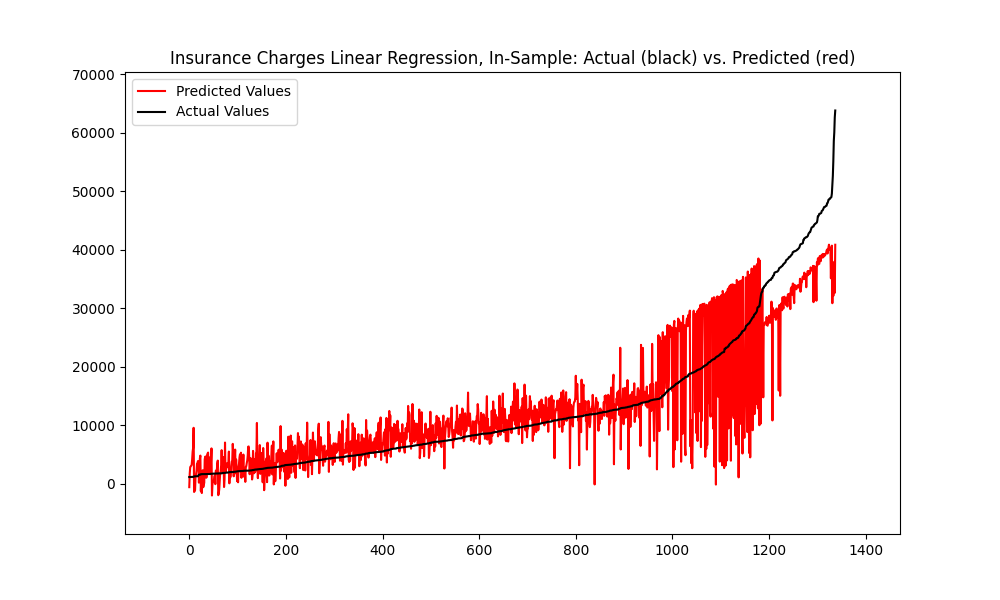
\includegraphics[width=\textwidth]{../Insurance_Charges_Plots/Reg_In_Sample.png}
     \end{subfigure}
     \hfill
     \begin{subfigure}[b]{0.49\textwidth}
         \centering
         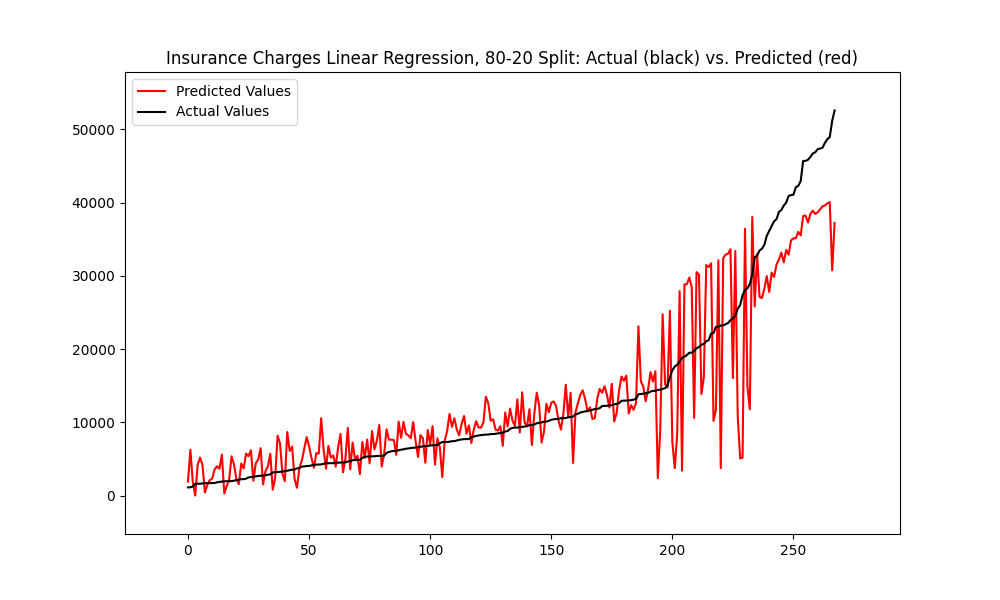
\includegraphics[width=\textwidth]{../Insurance_Charges_Plots/Reg_80_20.png}
     \end{subfigure}
     
     \caption{Insurance Charges Linear Regression Plots\\ Left: In-Sample, Right: Out-of-Sample\\ black: actual y-values, red: predicted y-values}
     \label{fig:Insurance Charges Linear Regression Plots}
\end{figure}

\begin{table}[H]
\centering
\caption{Insurance Charges Linear Regression}
\label{tab:Insurance Charges Linear Regression}
\begin{tabular}{|c|c|c|}\hline
Metric & In-Sample & 80-20 Split \\ \hline \hline
rSq & 0.7509 & 0.8 \\ \hline
rSqBar & 0.7494 & 0.7938 \\ \hline
sst & 1.961e+11 & 4.265e+10 \\ \hline
sse & 4.884e+10 & 8.53e+09 \\ \hline
sde & 6062 & 5739 \\ \hline
mse0 & 3.65e+07 & 3.183e+07 \\ \hline
rmse & 6042 & 5642 \\ \hline
mae & 4171 & 3933 \\ \hline
smape & 37.81 & 35.02 \\ \hline
m & 1338 & 268 \\ \hline
dfr & 9 & 9 \\ \hline
df & 1329 & 259 \\ \hline
fStat & 445.2 & 115.1 \\ \hline
aic & 2.332e+04 & 4648 \\ \hline
bic & 2.336e+04 & 4680 \\ \hline
\end{tabular}
\end{table}

\begin{table}[H]
\centering
\caption{Insurance Charges Linear Regression CV}
\label{tab:Insurance Charges Linear Regression CV}
\begin{tabular}{|c|c|c|c|c|c|}\hline
Metric & num folds & min & max & mean & stdev \\ \hline \hline
rSq & 5 & 0.6525 & 0.8 & 0.7401 & 0.05195 \\ \hline
rSqBar & 5 & 0.6418 & 0.7938 & 0.7321 & 0.05356 \\ \hline
sst & 5 & 2.986e+10 & 4.265e+10 & 3.902e+10 & 4.668e+09 \\ \hline
sse & 5 & 8.53e+09 & 1.192e+10 & 9.937e+09 & 1.194e+09 \\ \hline
sde & 5 & 5739 & 6798 & 6188 & 372.4 \\ \hline
mse0 & 5 & 3.183e+07 & 4.465e+07 & 3.714e+07 & 4.509e+06 \\ \hline
rmse & 5 & 5642 & 6682 & 6083 & 365.9 \\ \hline
mae & 5 & 3933 & 4559 & 4206 & 212.5 \\ \hline
smape & 5 & 35.02 & 41.32 & 38.03 & 2.113 \\ \hline
m & 5 & 267 & 268 & 267.6 & 0.4899 \\ \hline
dfr & 5 & 9 & 9 & 9 & 0 \\ \hline
df & 5 & 258 & 259 & 258.6 & 0.4899 \\ \hline
fStat & 5 & 54.05 & 115.1 & 86.05 & 21.39 \\ \hline
aic & 5 & 4648 & 4721 & 4680 & 26.77 \\ \hline
bic & 5 & 4680 & 4753 & 4713 & 26.76 \\ \hline
\end{tabular}
\end{table}

\subsubsection{Feature Selection}

\noindent Forward Selection: Null, smoker yes, age, bmi, region southwest, region northwest, region southeast, children, sex male

\begin{figure}[H]
     \centering
     \captionsetup{justification=centering}
     \begin{subfigure}[b]{0.49\textwidth}
         \centering
         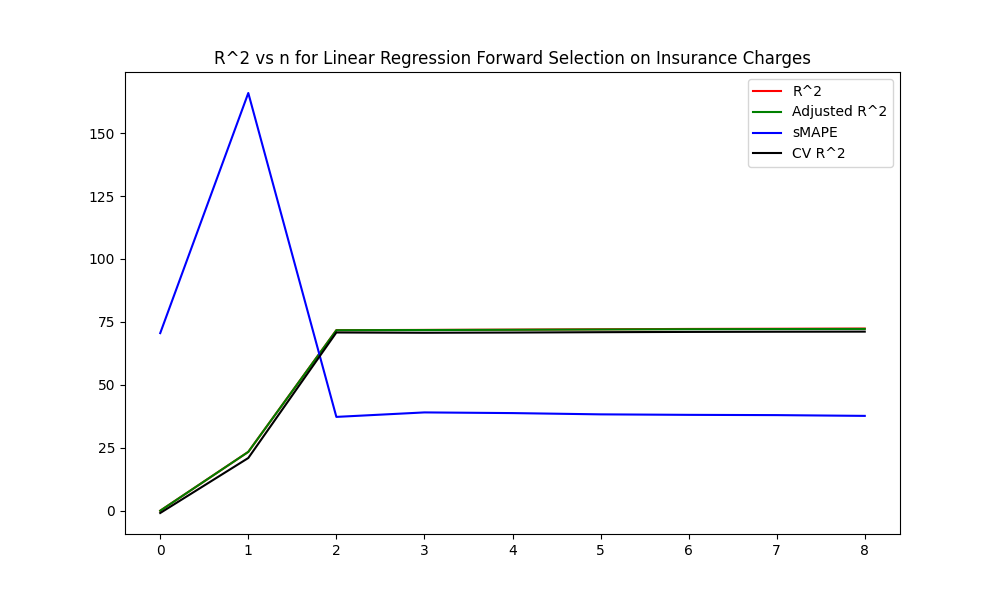
\includegraphics[width=\textwidth]{../Insurance_Charges_Plots/Reg_rSq_Forward.png}
     \end{subfigure}
     \hfill
     \begin{subfigure}[b]{0.49\textwidth}
         \centering
         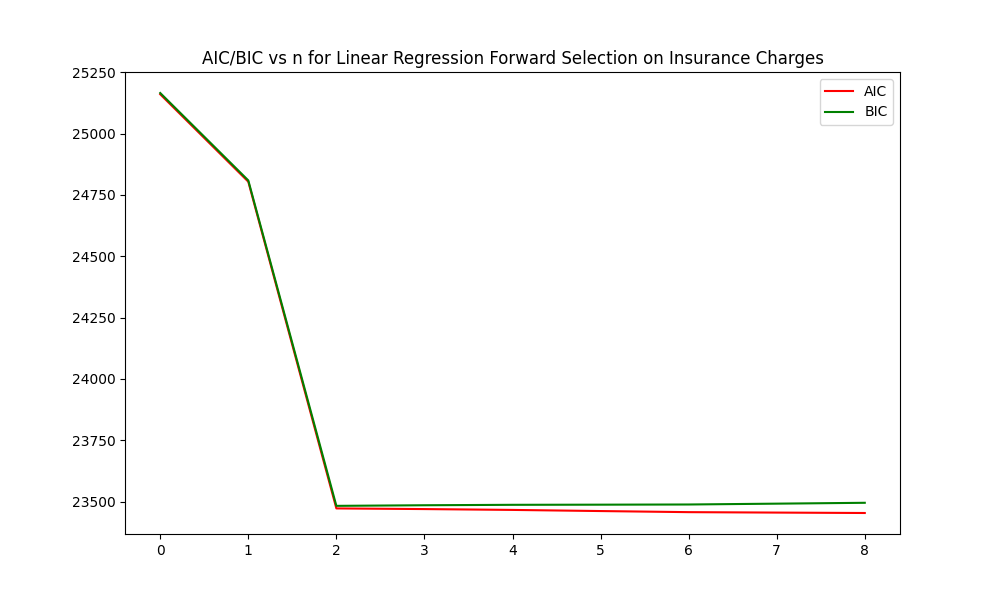
\includegraphics[width=\textwidth]{../Insurance_Charges_Plots/Reg_AIC_BIC_Forward.png}
     \end{subfigure}
     
     \caption{Insurance Charges Linear Regression Forward Selection Quality of Fit Metrics\\ Left: $R^2$, Right: AIC/BIC}
     \label{fig:Insurance Charges Linear Regression Forward Selection Quality of Fit Metrics}
\end{figure}

\noindent Backward Elimination Reversed: Null, smoker yes, age, bmi, region southwest, region northwest, region southeast, children, sex male

\begin{figure}[H]
     \centering
     \captionsetup{justification=centering}
     \begin{subfigure}[b]{0.49\textwidth}
         \centering
         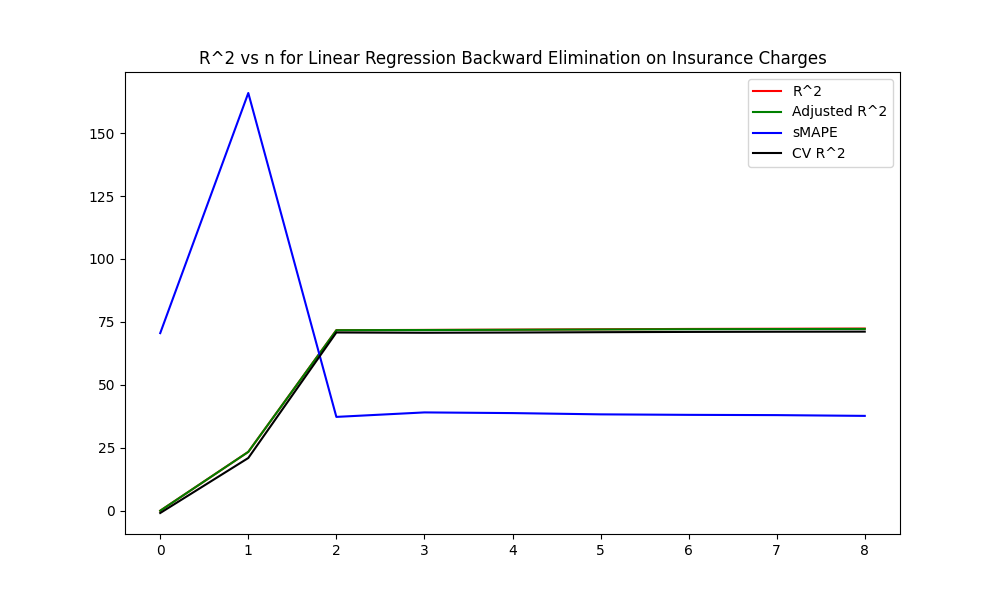
\includegraphics[width=\textwidth]{../Insurance_Charges_Plots/Reg_rSq_Backward.png}
     \end{subfigure}
     \hfill
     \begin{subfigure}[b]{0.49\textwidth}
         \centering
         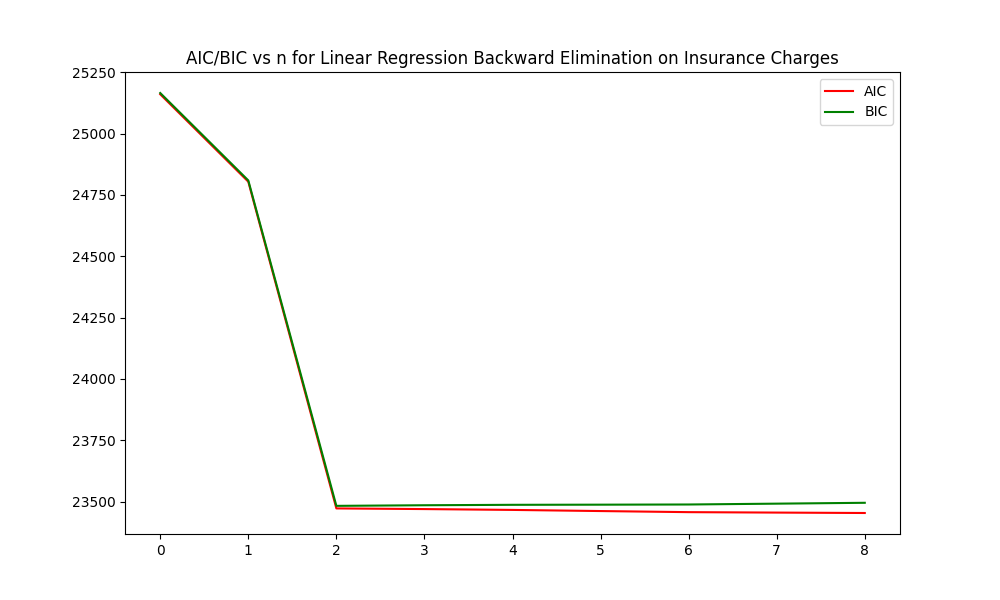
\includegraphics[width=\textwidth]{../Insurance_Charges_Plots/Reg_AIC_BIC_Backward.png}
     \end{subfigure}
     
     \caption{Insurance Charges Linear Regression Backward Elimination Quality of Fit Metrics\\ Left: $R^2$, Right: AIC/BIC}
     \label{fig:Insurance Charges Linear Regression Backward Elimination Quality of Fit Metrics}
\end{figure}

\noindent Stepwise Selection: Null, smoker yes, age, bmi, region southwest, region northwest, region southeast, children, sex male

\begin{figure}[H]
     \centering
     \captionsetup{justification=centering}
     \begin{subfigure}[b]{0.49\textwidth}
         \centering
         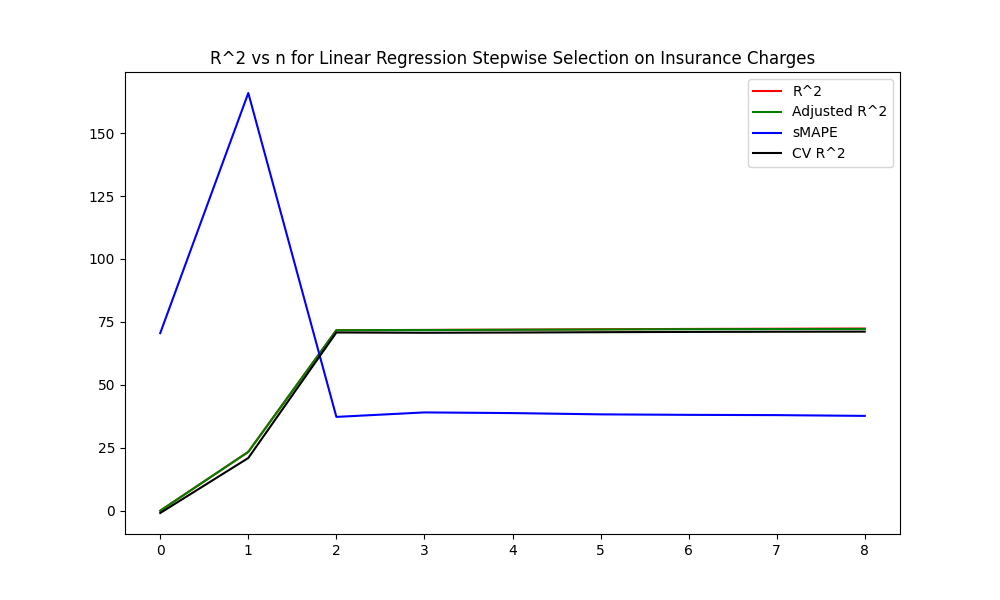
\includegraphics[width=\textwidth]{../Insurance_Charges_Plots/Reg_rSq_Stepwise.png}
     \end{subfigure}
     \hfill
     \begin{subfigure}[b]{0.49\textwidth}
         \centering
         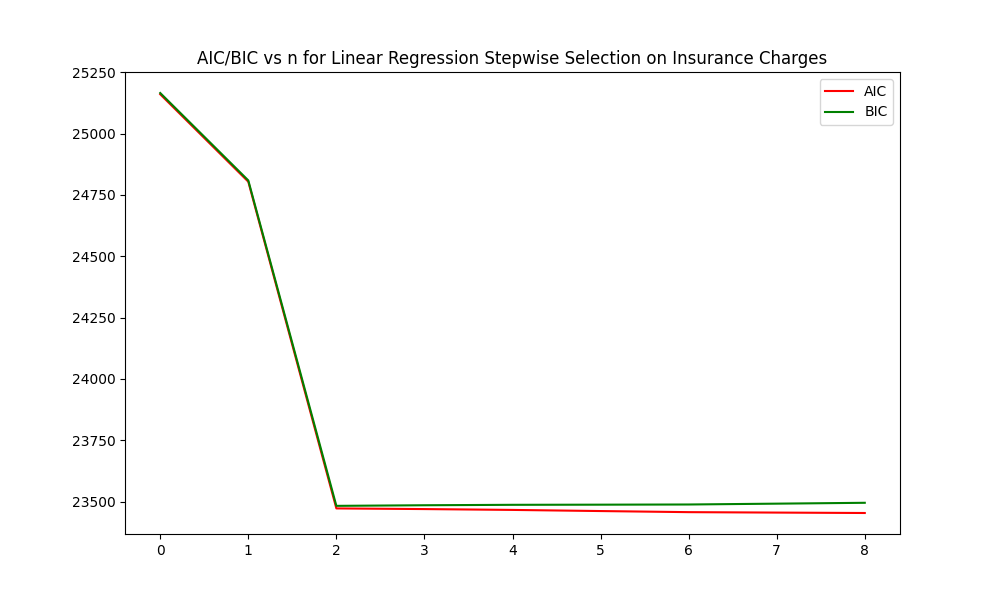
\includegraphics[width=\textwidth]{../Insurance_Charges_Plots/Reg_AIC_BIC_Stepwise.png}
     \end{subfigure}
     
     \caption{Insurance Charges Linear Regression Stepwise Selection Quality of Fit Metrics\\ Left: $R^2$, Right: AIC/BIC}
     \label{fig:Insurance Charges Linear Regression Stepwise Selection Quality of Fit Metrics}
\end{figure}

%%%%%%%%%%%%%%%%%%%%%%%%%%%%%%%%%%%%%%%%%%%%%%%%%%%%%%%%%%%%
%%%%%%%%%%%%%%%%%%%%%%%%%%%%%%%%%%%%%%%%%%%%%%%%%%%%%%%%%%%%
%%%%%%%%%%%%%%%%%%%%%%%%%%%%%%%%%%%%%%%%%%%%%%%%%%%%%%%%%%%%
%%%%%%%%%%%%%%%%%%%%%%%%%%%%%%%%%%%%%%%%%%%%%%%%%%%%%%%%%%%%
%%%%%%%%%%%%%%%%%%%%%%%%%%%%%%%%%%%%%%%%%%%%%%%%%%%%%%%%%%%%
%%%%%%%%%%%%%%%%%%%%%%%%%%%%%%%%%%%%%%%%%%%%%%%%%%%%%%%%%%%%

\subsection{Ridge Regression}

\subsubsection{Quality of Fit}

Insurance Charges Ridge alpha Used: 0.009000000000000001

\begin{figure}[H]
     \centering
     \captionsetup{justification=centering}
     \begin{subfigure}[b]{0.49\textwidth}
         \centering
         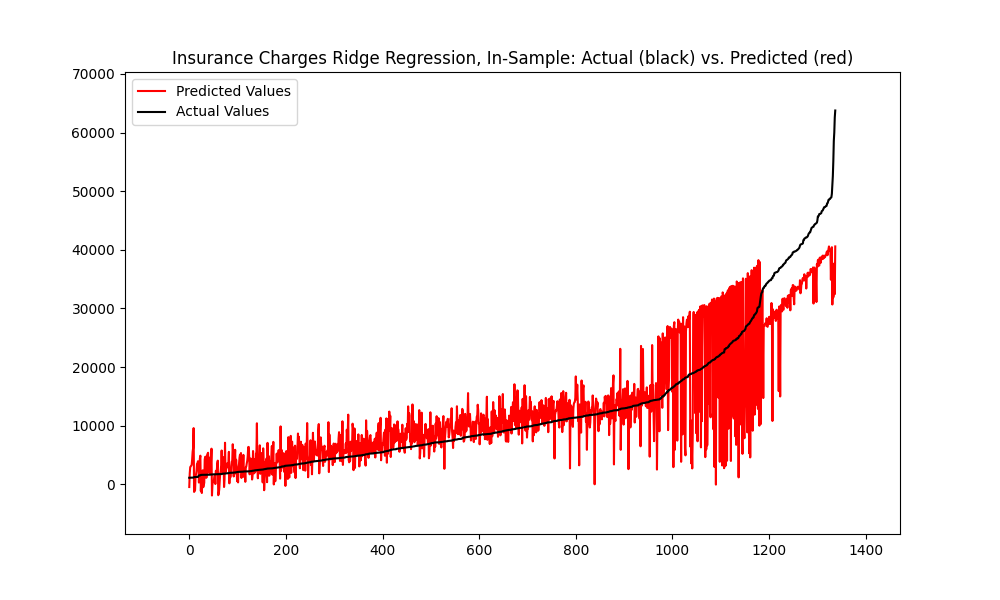
\includegraphics[width=\textwidth]{../Insurance_Charges_Plots/Ridge_In_Sample.png}
     \end{subfigure}
     \hfill
     \begin{subfigure}[b]{0.49\textwidth}
         \centering
         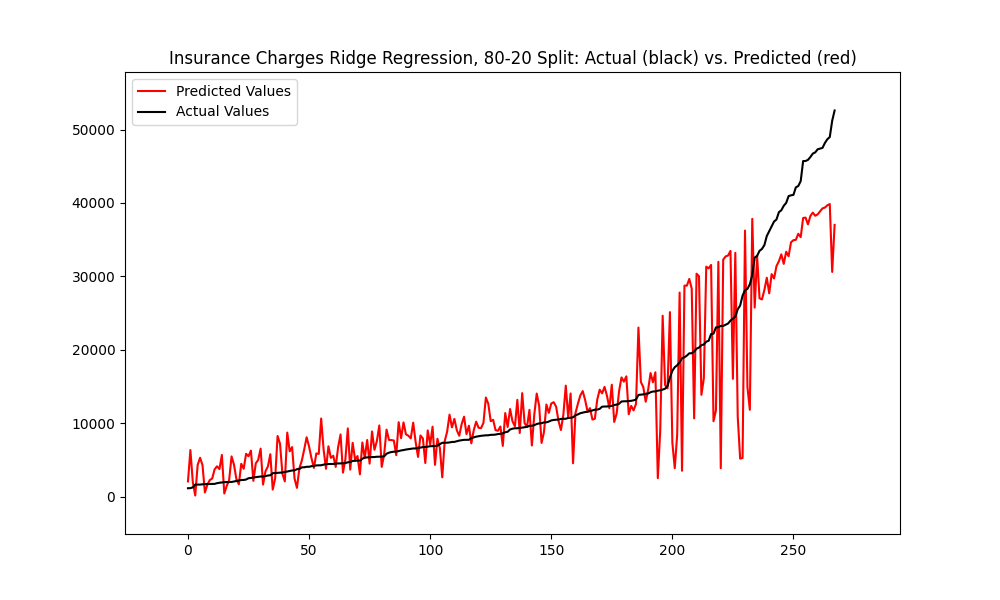
\includegraphics[width=\textwidth]{../Insurance_Charges_Plots/Ridge_80_20.png}
     \end{subfigure}
     
     \caption{Insurance Charges Ridge Regression Plots\\ Left: In-Sample, Right: Out-of-Sample\\ black: actual y-values, red: predicted y-values}
     \label{fig:Insurance Charges Ridge Regression Plots}
\end{figure}

\begin{table}[H]
\centering
\caption{Insurance Charges Ridge Regression}
\label{tab:Insurance Charges Ridge Regression}
\begin{tabular}{|c|c|c|}\hline
Metric & In-Sample & 80-20 Split \\ \hline \hline
rSq & 0.7509 & 0.7993 \\ \hline
rSqBar & 0.7495 & 0.7939 \\ \hline
sst & 1.961e+11 & 4.265e+10 \\ \hline
sse & 4.885e+10 & 8.561e+09 \\ \hline
sde & 6061 & 5738 \\ \hline
mse0 & 3.651e+07 & 3.194e+07 \\ \hline
rmse & 6042 & 5652 \\ \hline
mae & 4182 & 3951 \\ \hline
smape & 37.68 & 34.84 \\ \hline
m & 1338 & 268 \\ \hline
dfr & 8 & 8 \\ \hline
df & 1330 & 260 \\ \hline
fStat & 501 & 129.4 \\ \hline
aic & 2.331e+04 & 4647 \\ \hline
bic & 2.336e+04 & 4676 \\ \hline
\end{tabular}
\end{table}

\begin{table}[H]
\centering
\caption{Insurance Charges Ridge Regression CV}
\label{tab:Insurance Charges Ridge Regression CV}
\begin{tabular}{|c|c|c|c|c|c|}\hline
Metric & num folds & min & max & mean & stdev \\ \hline \hline
rSq & 5 & 0.6543 & 0.7993 & 0.7402 & 0.05105 \\ \hline
rSqBar & 5 & 0.645 & 0.7939 & 0.7332 & 0.05242 \\ \hline
sst & 5 & 2.986e+10 & 4.265e+10 & 3.902e+10 & 4.668e+09 \\ \hline
sse & 5 & 8.561e+09 & 1.191e+10 & 9.938e+09 & 1.173e+09 \\ \hline
sde & 5 & 5738 & 6780 & 6177 & 365 \\ \hline
mse0 & 5 & 3.194e+07 & 4.459e+07 & 3.714e+07 & 4.432e+06 \\ \hline
rmse & 5 & 5652 & 6678 & 6084 & 359.4 \\ \hline
mae & 5 & 3951 & 4562 & 4217 & 207.7 \\ \hline
smape & 5 & 34.84 & 41.02 & 37.88 & 2.054 \\ \hline
m & 5 & 267 & 268 & 267.6 & 0.4899 \\ \hline
dfr & 5 & 8 & 8 & 8 & 0 \\ \hline
df & 5 & 259 & 260 & 259.6 & 0.4899 \\ \hline
fStat & 5 & 61.5 & 129.4 & 97.06 & 23.77 \\ \hline
aic & 5 & 4647 & 4719 & 4678 & 26.08 \\ \hline
bic & 5 & 4676 & 4747 & 4707 & 26.07 \\ \hline
\end{tabular}
\end{table}

\subsubsection{Feature Selection}

\noindent Forward Selection: Null, smoker yes, age, bmi, children, region southeast, region southwest, region northwest, sex male

\begin{figure}[H]
     \centering
     \captionsetup{justification=centering}
     \begin{subfigure}[b]{0.49\textwidth}
         \centering
         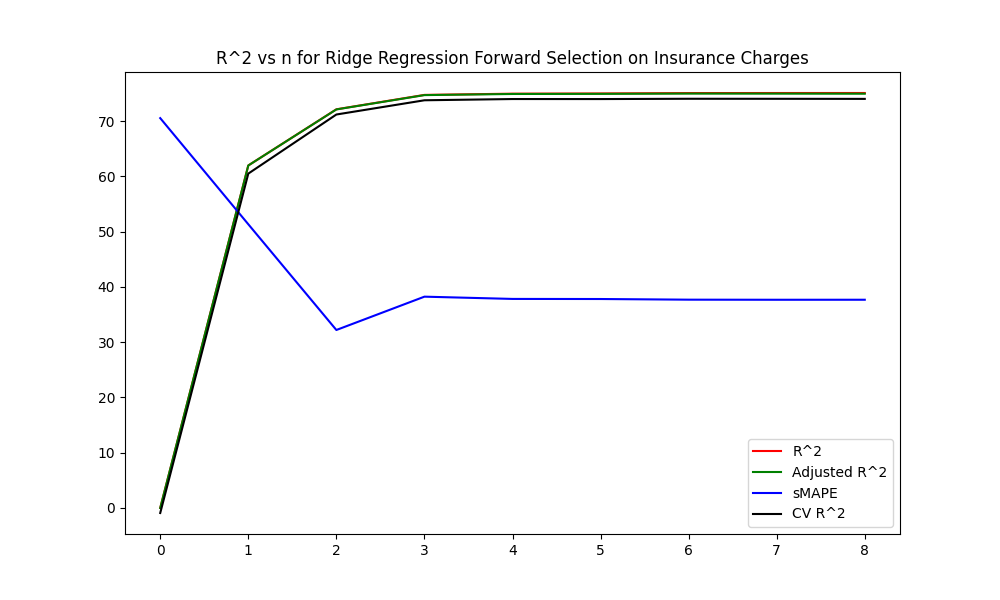
\includegraphics[width=\textwidth]{../Insurance_Charges_Plots/Ridge_rSq_Forward.png}
     \end{subfigure}
     \hfill
     \begin{subfigure}[b]{0.49\textwidth}
         \centering
         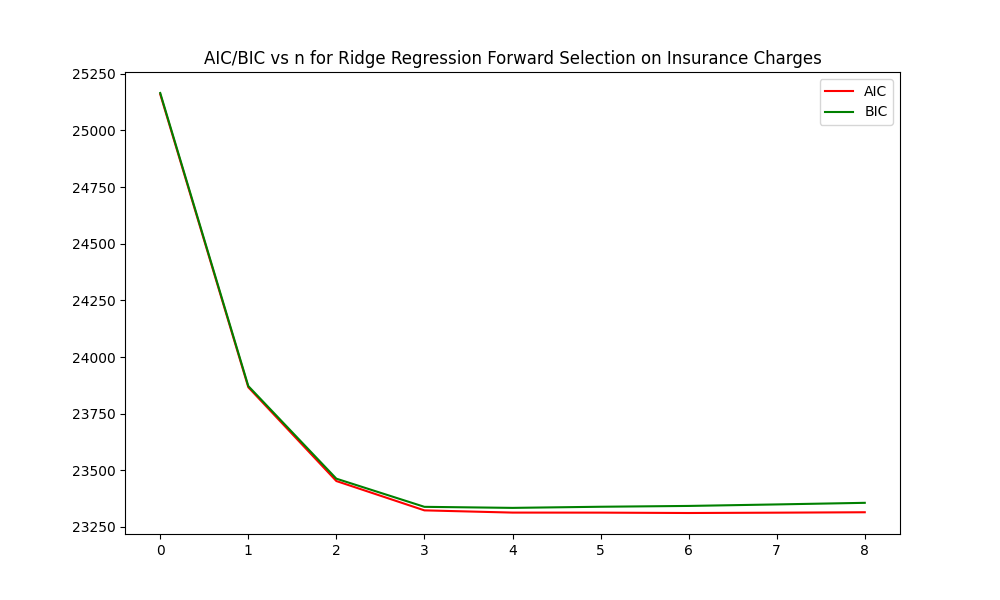
\includegraphics[width=\textwidth]{../Insurance_Charges_Plots/Ridge_AIC_BIC_Forward.png}
     \end{subfigure}
     
     \caption{Insurance Charges Ridge Regression Forward Selection Quality of Fit Metrics\\ Left: $R^2$, Right: AIC/BIC}
     \label{fig:Insurance Charges Ridge Regression Forward Selection Quality of Fit Metrics}
\end{figure}

\noindent Backward Elimination Reversed: Null, smoker yes, age, bmi, children, region southeast, region southwest, region northwest, sex male

\begin{figure}[H]
     \centering
     \captionsetup{justification=centering}
     \begin{subfigure}[b]{0.49\textwidth}
         \centering
         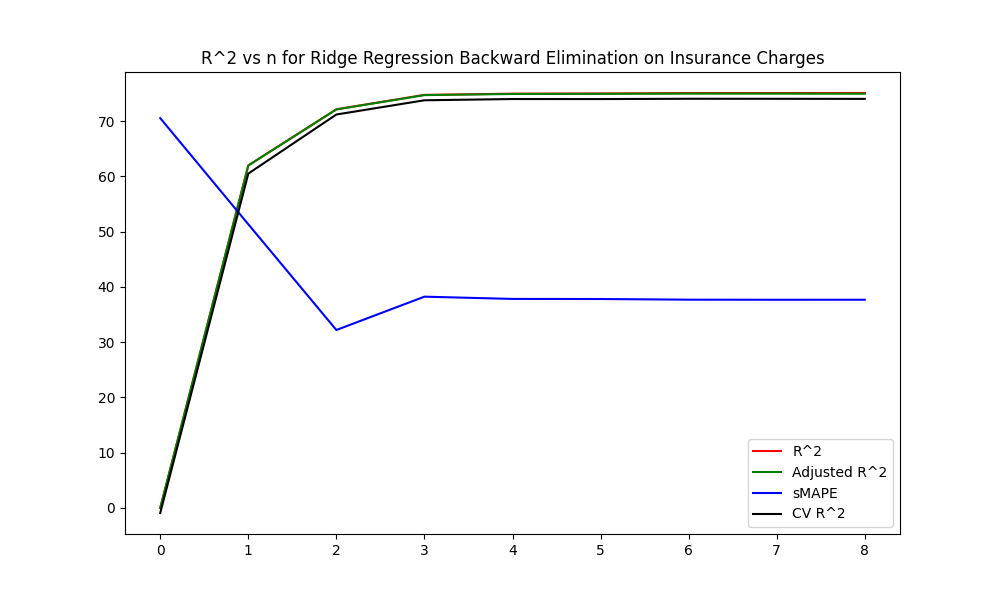
\includegraphics[width=\textwidth]{../Insurance_Charges_Plots/Ridge_rSq_Backward.png}
     \end{subfigure}
     \hfill
     \begin{subfigure}[b]{0.49\textwidth}
         \centering
         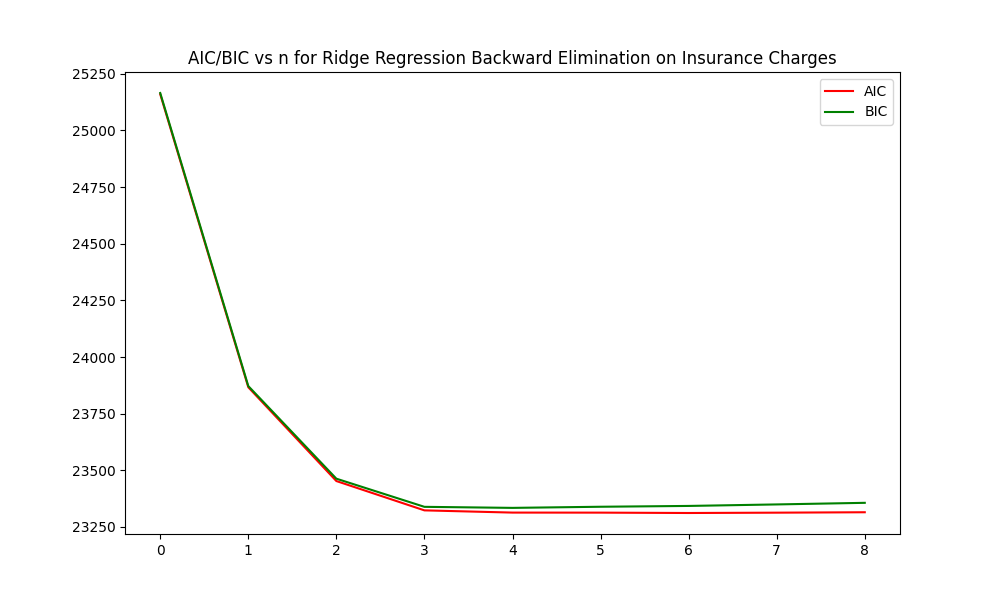
\includegraphics[width=\textwidth]{../Insurance_Charges_Plots/Ridge_AIC_BIC_Backward.png}
     \end{subfigure}
     
     \caption{Insurance Charges Ridge Regression  Backward Elimination Quality of Fit Metrics\\ Left: $R^2$, Right: AIC/BIC}
     \label{fig:Insurance Charges Ridge Regression  Backward Elimination Quality of Fit Metrics}
\end{figure}

\noindent Stepwise Selection: Null, smoker yes, age, bmi, children, region southeast, region southwest

\begin{figure}[H]
     \centering
     \captionsetup{justification=centering}
     \begin{subfigure}[b]{0.49\textwidth}
         \centering
         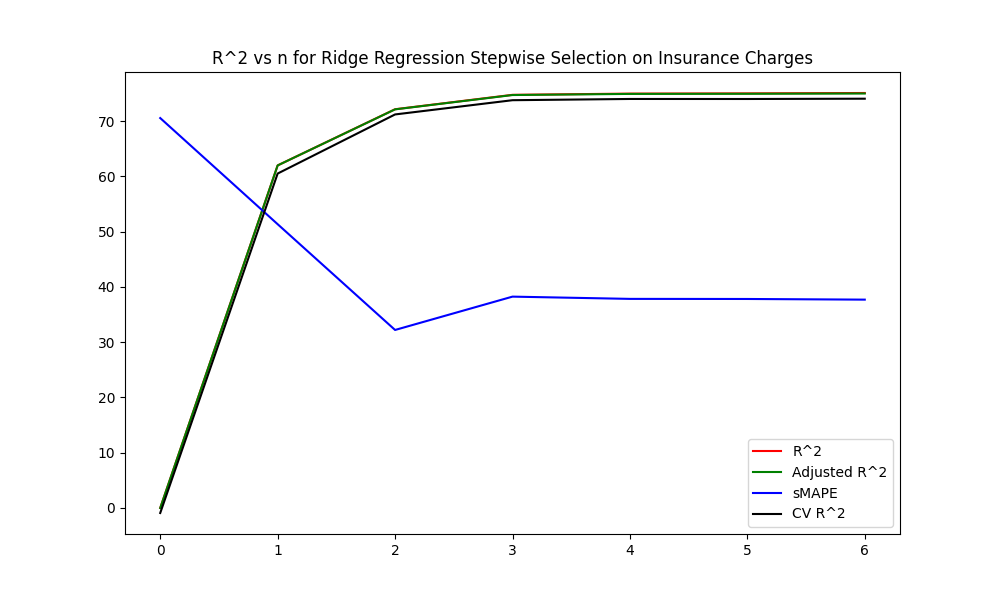
\includegraphics[width=\textwidth]{../Insurance_Charges_Plots/Ridge_rSq_Stepwise.png}
     \end{subfigure}
     \hfill
     \begin{subfigure}[b]{0.49\textwidth}
         \centering
         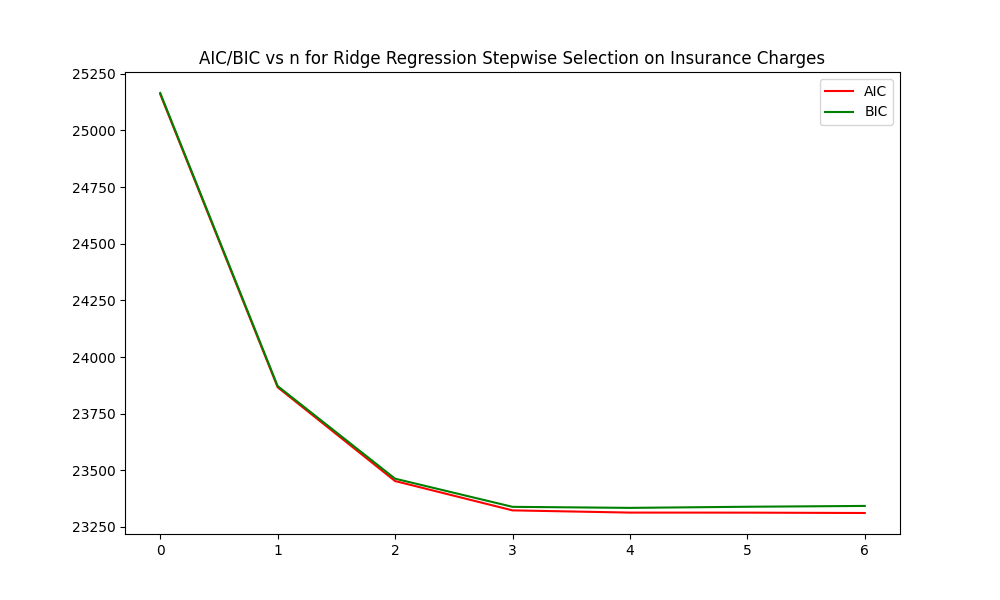
\includegraphics[width=\textwidth]{../Insurance_Charges_Plots/Ridge_AIC_BIC_Stepwise.png}
     \end{subfigure}
     
     \caption{Insurance Charges Ridge Regression Stepwise Selection Quality of Fit Metrics\\ Left: $R^2$, Right: AIC/BIC}
     \label{fig:Insurance Charges Ridge Regression Stepwise Selection Quality of Fit Metrics}
\end{figure}

%%%%%%%%%%%%%%%%%%%%%%%%%%%%%%%%%%%%%%%%%%%%%%%%%%%%%%%%%%%%
%%%%%%%%%%%%%%%%%%%%%%%%%%%%%%%%%%%%%%%%%%%%%%%%%%%%%%%%%%%%
%%%%%%%%%%%%%%%%%%%%%%%%%%%%%%%%%%%%%%%%%%%%%%%%%%%%%%%%%%%%
%%%%%%%%%%%%%%%%%%%%%%%%%%%%%%%%%%%%%%%%%%%%%%%%%%%%%%%%%%%%
%%%%%%%%%%%%%%%%%%%%%%%%%%%%%%%%%%%%%%%%%%%%%%%%%%%%%%%%%%%%
%%%%%%%%%%%%%%%%%%%%%%%%%%%%%%%%%%%%%%%%%%%%%%%%%%%%%%%%%%%%

\subsection{Lasso Regression}

\subsubsection{Quality of Fit}

Insurance Charges Lasso alpha Used: 0.0008

\noindent Insurance Charges Lasso Selected Features: age, bmi, children, sex male, smoker yes, region northwest, region southeast, region southwest

\begin{figure}[H]
     \centering
     \captionsetup{justification=centering}
     \begin{subfigure}[b]{0.49\textwidth}
         \centering
         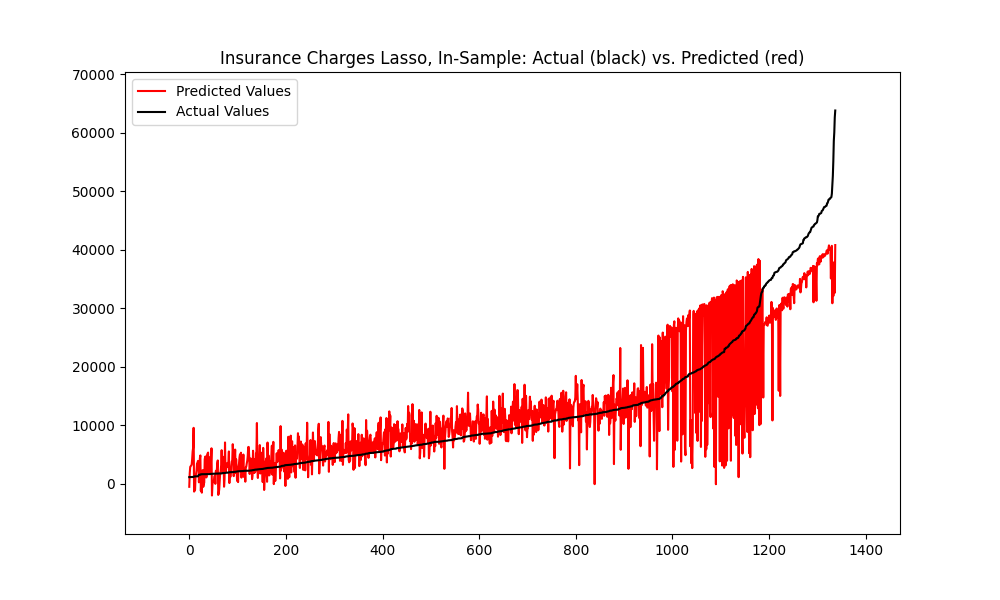
\includegraphics[width=\textwidth]{../Insurance_Charges_Plots/Lasso_In_Sample.png}
     \end{subfigure}
     \hfill
     \begin{subfigure}[b]{0.49\textwidth}
         \centering
         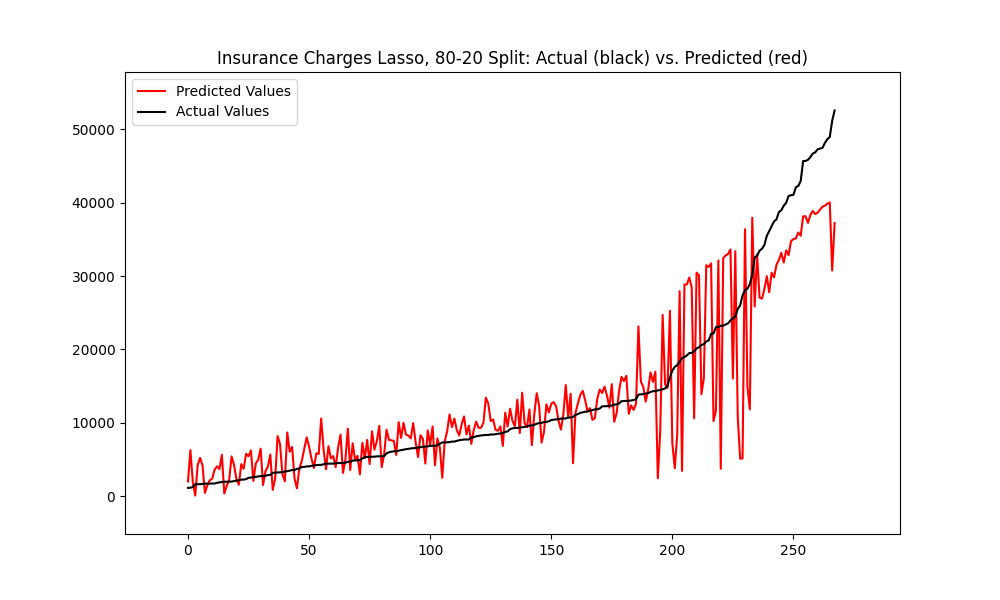
\includegraphics[width=\textwidth]{../Insurance_Charges_Plots/Lasso_80_20.png}
     \end{subfigure}
     
     \caption{Insurance Charges Lasso Regression Plots\\ Left: In-Sample, Right: Out-of-Sample\\ black: actual y-values, red: predicted y-values}
     \label{fig:Insurance Charges Lasso Regression Plots}
\end{figure}

\begin{table}[H]
\centering
\caption{Insurance Charges Lasso Regression}
\label{tab:Insurance Charges Lasso Regression}
\begin{tabular}{|c|c|c|}\hline
Metric & In-Sample & 80-20 Split \\ \hline \hline
rSq & 0.7509 & 0.7997 \\ \hline
rSqBar & 0.7496 & 0.7943 \\ \hline
sst & 1.961e+11 & 4.265e+10 \\ \hline
sse & 4.884e+10 & 8.541e+09 \\ \hline
sde & 6060 & 5732 \\ \hline
mse0 & 3.65e+07 & 3.187e+07 \\ \hline
rmse & 6042 & 5645 \\ \hline
mae & 4170 & 3936 \\ \hline
smape & 37.72 & 35.01 \\ \hline
m & 1338 & 268 \\ \hline
dfr & 8 & 8 \\ \hline
df & 1330 & 260 \\ \hline
fStat & 501.2 & 129.8 \\ \hline
aic & 2.331e+04 & 4646 \\ \hline
bic & 2.336e+04 & 4675 \\ \hline
\end{tabular}
\end{table}

\begin{table}[H]
\centering
\caption{Insurance Charges Lasso Regression CV}
\label{tab:Insurance Charges Lasso Regression CV}
\begin{tabular}{|c|c|c|c|c|c|}\hline
Metric & num folds & min & max & mean & stdev \\ \hline \hline
rSq & 5 & 0.6528 & 0.7997 & 0.7401 & 0.05184 \\ \hline
rSqBar & 5 & 0.6434 & 0.7943 & 0.7331 & 0.05324 \\ \hline
sst & 5 & 2.986e+10 & 4.265e+10 & 3.902e+10 & 4.668e+09 \\ \hline
sse & 5 & 8.541e+09 & 1.192e+10 & 9.938e+09 & 1.192e+09 \\ \hline
sde & 5 & 5732 & 6785 & 6176 & 371 \\ \hline
mse0 & 5 & 3.187e+07 & 4.465e+07 & 3.714e+07 & 4.502e+06 \\ \hline
rmse & 5 & 5645 & 6682 & 6083 & 365.3 \\ \hline
mae & 5 & 3936 & 4560 & 4206 & 212.2 \\ \hline
smape & 5 & 35.01 & 41.12 & 37.94 & 2.044 \\ \hline
m & 5 & 267 & 268 & 267.6 & 0.4899 \\ \hline
dfr & 5 & 8 & 8 & 8 & 0 \\ \hline
df & 5 & 259 & 260 & 259.6 & 0.4899 \\ \hline
fStat & 5 & 61.09 & 129.8 & 97.17 & 24.09 \\ \hline
aic & 5 & 4646 & 4719 & 4678 & 26.69 \\ \hline
bic & 5 & 4675 & 4748 & 4707 & 26.68 \\ \hline
\end{tabular}
\end{table}

\subsubsection{Feature Selection}

\noindent Forward Selection: Null, smoker yes, age, bmi, children, region southeast, region southwest, region northwest, sex male

\begin{figure}[H]
     \centering
     \captionsetup{justification=centering}
     \begin{subfigure}[b]{0.49\textwidth}
         \centering
         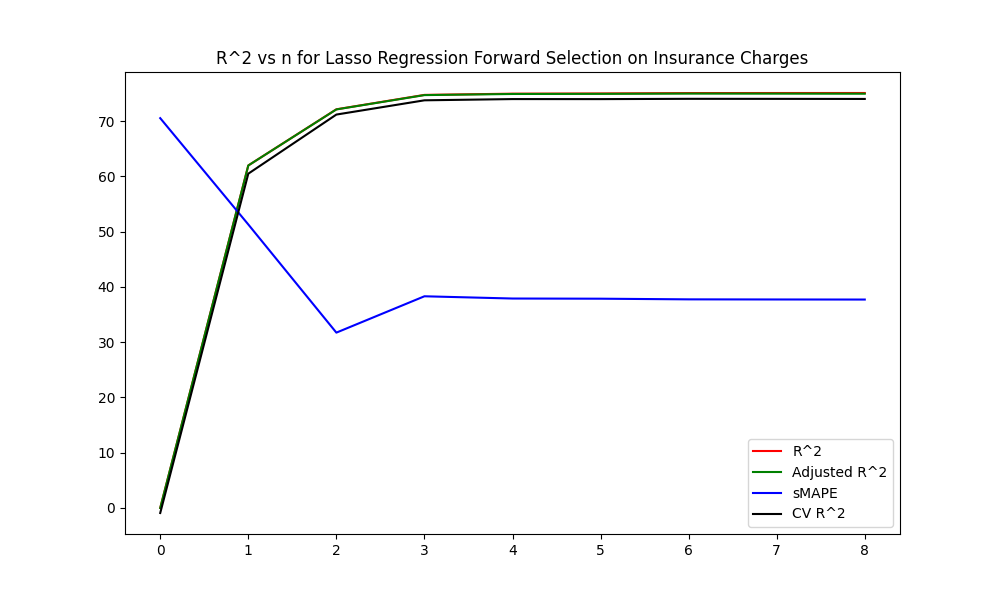
\includegraphics[width=\textwidth]{../Insurance_Charges_Plots/Lasso_rSq_Forward.png}
     \end{subfigure}
     \hfill
     \begin{subfigure}[b]{0.49\textwidth}
         \centering
         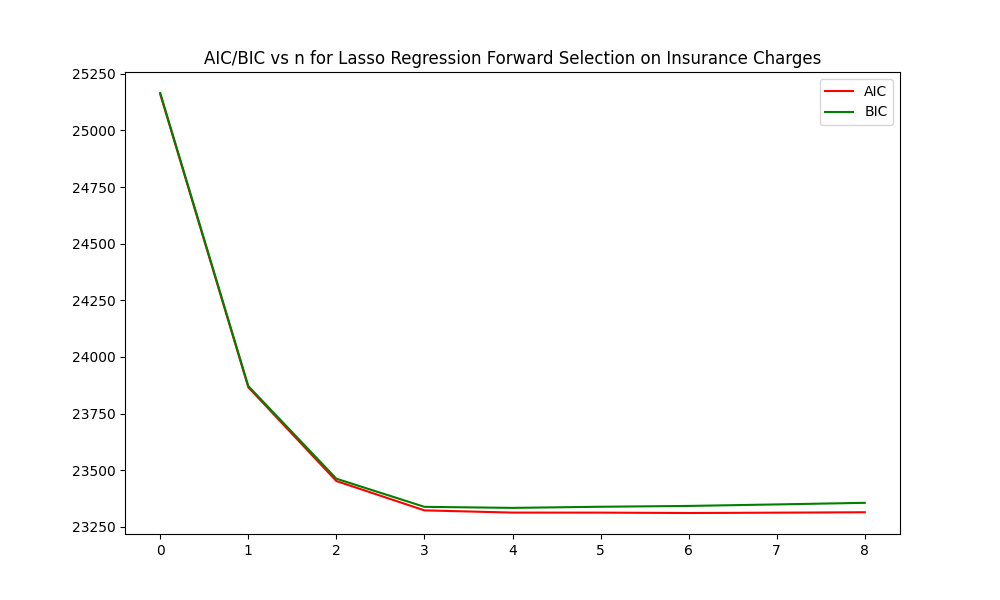
\includegraphics[width=\textwidth]{../Insurance_Charges_Plots/Lasso_AIC_BIC_Forward.png}
     \end{subfigure}
     
     \caption{Insurance Charges Lasso Regression Forward Selection Quality of Fit Metrics\\ Left: $R^2$, Right: AIC/BIC}
     \label{fig:Insurance Charges Lasso Regression Forward Selection Quality of Fit Metrics}
\end{figure}

\noindent Backward Elimination Reversed: Null, smoker yes, age, bmi, children, region southeast, region southwest, sex male, region northwest

\begin{figure}[H]
     \centering
     \captionsetup{justification=centering}
     \begin{subfigure}[b]{0.49\textwidth}
         \centering
         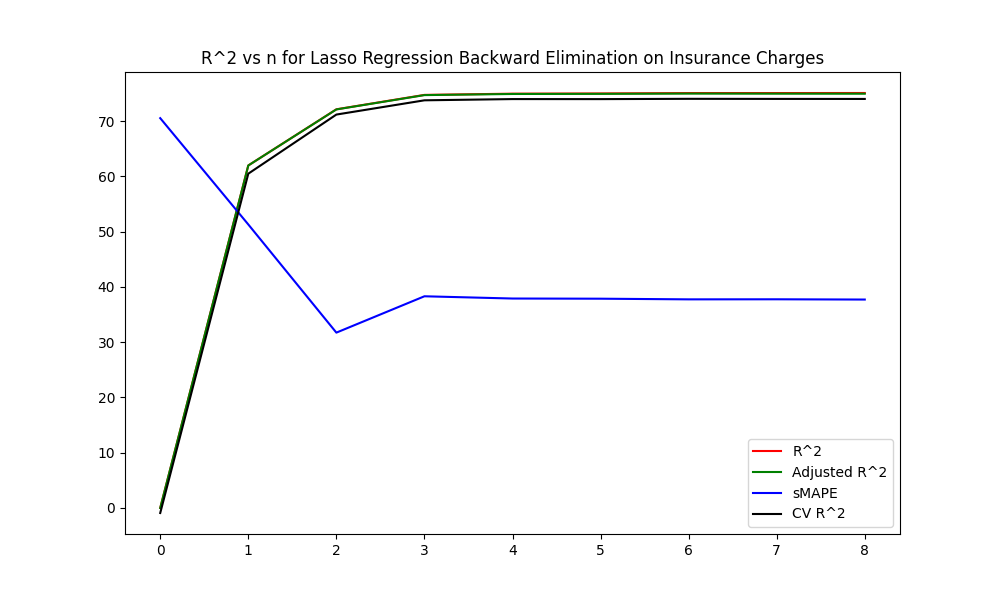
\includegraphics[width=\textwidth]{../Insurance_Charges_Plots/Lasso_rSq_Backward.png}
     \end{subfigure}
     \hfill
     \begin{subfigure}[b]{0.49\textwidth}
         \centering
         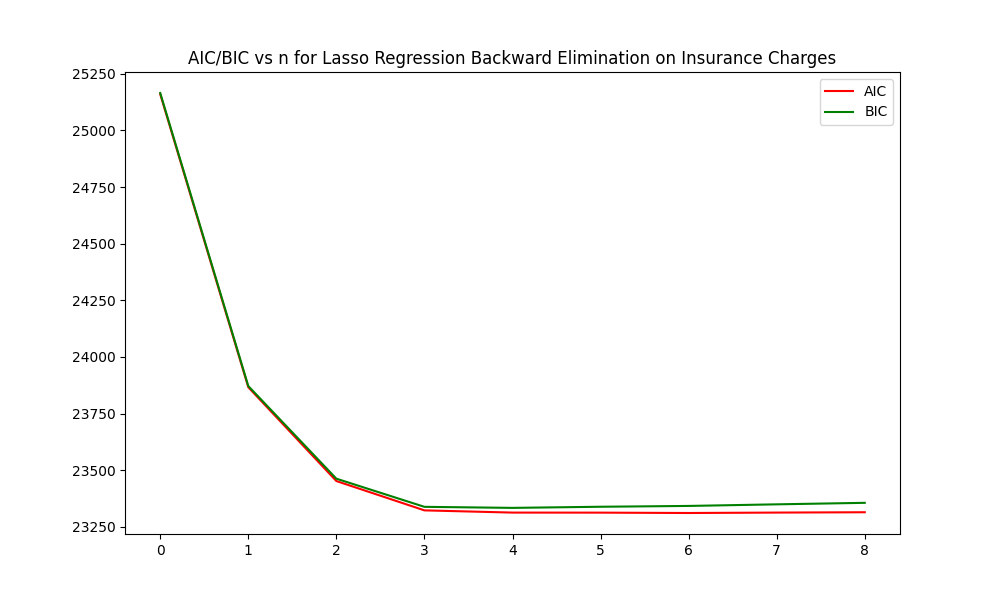
\includegraphics[width=\textwidth]{../Insurance_Charges_Plots/Lasso_AIC_BIC_Backward.png}
     \end{subfigure}
     
     \caption{Insurance Charges Lasso Regression Backward Elimination Quality of Fit Metrics\\ Left: $R^2$, Right: AIC/BIC}
     \label{fig:Insurance Charges Lasso Regression Backward Elimination Quality of Fit Metrics}
\end{figure}

\noindent Stepwise Selection: Null, smoker yes, age, bmi, children, region southeast, region southwest

\begin{figure}[H]
     \centering
     \captionsetup{justification=centering}
     \begin{subfigure}[b]{0.49\textwidth}
         \centering
         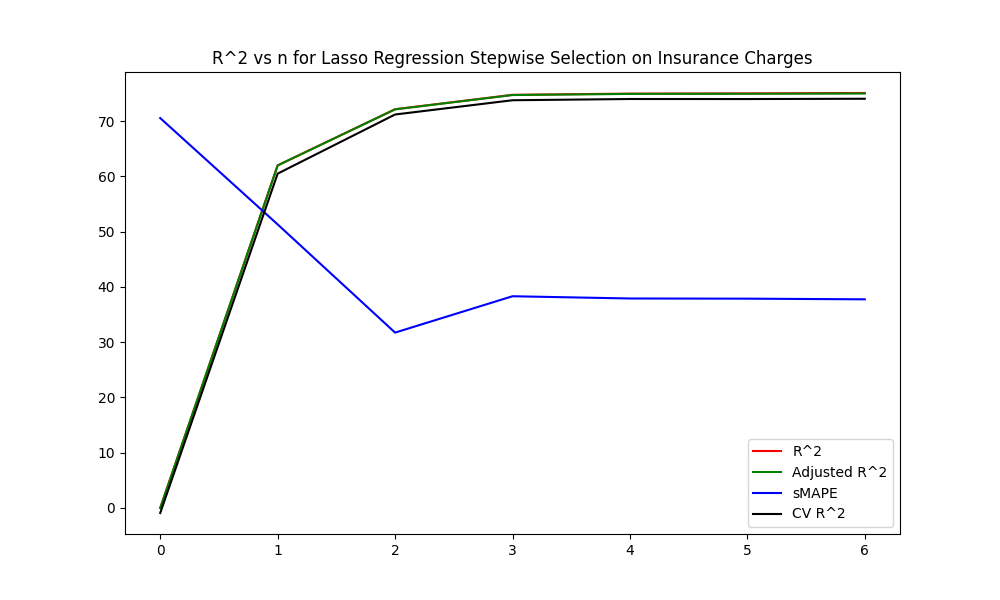
\includegraphics[width=\textwidth]{../Insurance_Charges_Plots/Lasso_rSq_Stepwise.png}
     \end{subfigure}
     \hfill
     \begin{subfigure}[b]{0.49\textwidth}
         \centering
         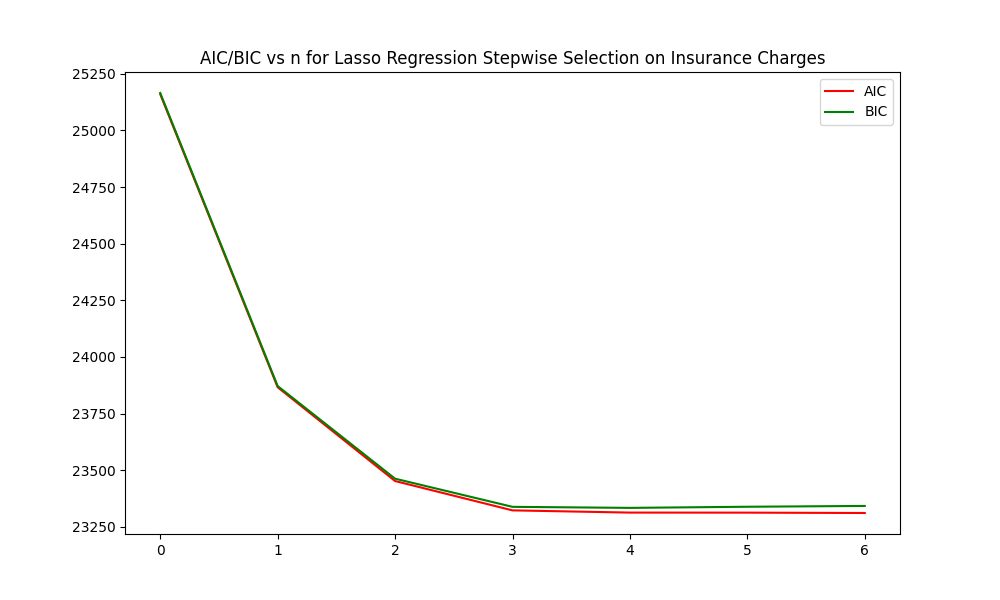
\includegraphics[width=\textwidth]{../Insurance_Charges_Plots/Lasso_AIC_BIC_Stepwise.png}
     \end{subfigure}
     
     \caption{Insurance Charges Lasso Regression Stepwise Selection Quality of Fit Metrics\\ Left: $R^2$, Right: AIC/BIC}
     \label{fig:Insurance Charges Lasso Regression Stepwise Selection Quality of Fit Metrics}
\end{figure}

%%%%%%%%%%%%%%%%%%%%%%%%%%%%%%%%%%%%%%%%%%%%%%%%%%%%%%%%%%%%
%%%%%%%%%%%%%%%%%%%%%%%%%%%%%%%%%%%%%%%%%%%%%%%%%%%%%%%%%%%%
%%%%%%%%%%%%%%%%%%%%%%%%%%%%%%%%%%%%%%%%%%%%%%%%%%%%%%%%%%%%
%%%%%%%%%%%%%%%%%%%%%%%%%%%%%%%%%%%%%%%%%%%%%%%%%%%%%%%%%%%%
%%%%%%%%%%%%%%%%%%%%%%%%%%%%%%%%%%%%%%%%%%%%%%%%%%%%%%%%%%%%
%%%%%%%%%%%%%%%%%%%%%%%%%%%%%%%%%%%%%%%%%%%%%%%%%%%%%%%%%%%%

\subsection{Sqrt Transformation}

\subsubsection{Quality of Fit}

\begin{figure}[H]
     \centering
     \captionsetup{justification=centering}
     \begin{subfigure}[b]{0.49\textwidth}
         \centering
         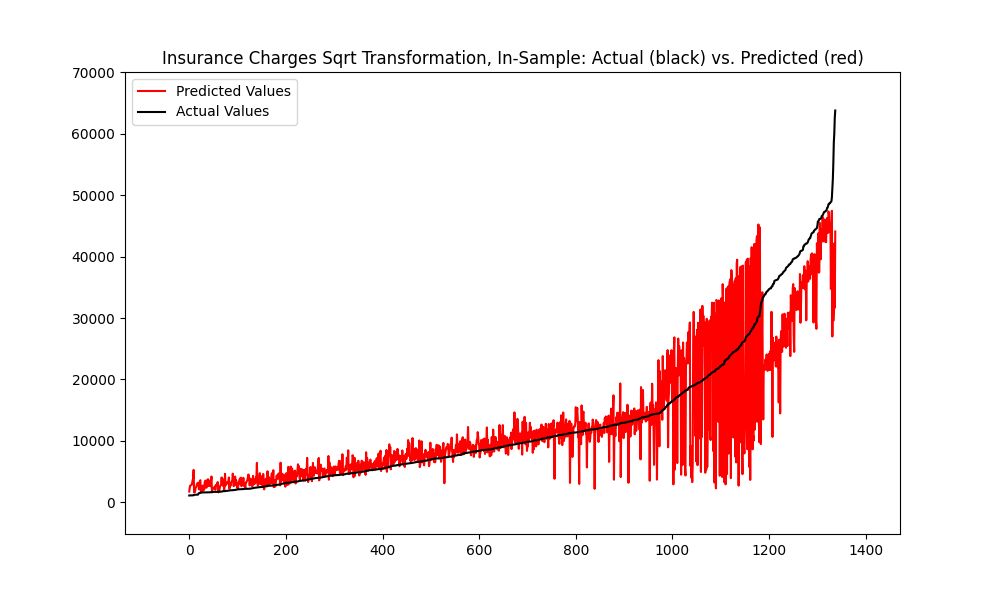
\includegraphics[width=\textwidth]{../Insurance_Charges_Plots/Sqrt_In_Sample.png}
     \end{subfigure}
     \hfill
     \begin{subfigure}[b]{0.49\textwidth}
         \centering
         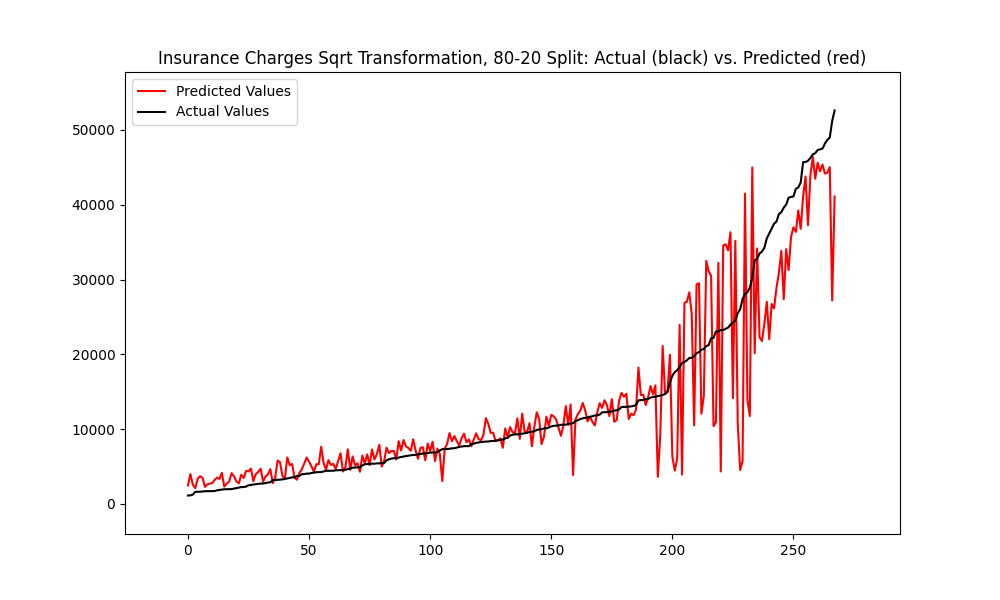
\includegraphics[width=\textwidth]{../Insurance_Charges_Plots/Sqrt_80_20.png}
     \end{subfigure}
     
     \caption{Insurance Charges Sqrt Transformation Plots\\ Left: In-Sample, Right: Out-of-Sample\\ black: actual y-values, red: predicted y-values}
     \label{fig:Insurance Charges Sqrt Transformation Plots}
\end{figure}

\begin{table}[H]
\centering
\caption{Insurance Charges Sqrt Transformation}
\label{tab:Insurance Charges Sqrt Transformation}
\begin{tabular}{|c|c|c|}\hline
Metric & In-Sample & 80-20 Split \\ \hline \hline
rSq & 0.7527 & 0.8077 \\ \hline
rSqBar & 0.7512 & 0.8017 \\ \hline
sst & 1.961e+11 & 4.265e+10 \\ \hline
sse & 4.85e+10 & 8.202e+09 \\ \hline
sde & 6041 & 5627 \\ \hline
mse0 & 3.625e+07 & 3.06e+07 \\ \hline
rmse & 6020 & 5532 \\ \hline
mae & 3614 & 3316 \\ \hline
smape & 27.69 & 26.47 \\ \hline
m & 1338 & 268 \\ \hline
dfr & 9 & 9 \\ \hline
df & 1329 & 259 \\ \hline
fStat & 449.3 & 120.9 \\ \hline
aic & 2.331e+04 & 4637 \\ \hline
bic & 2.335e+04 & 4670 \\ \hline
\end{tabular}
\end{table}

\begin{table}[H]
\centering
\caption{Insurance Charges Sqrt Transformation CV}
\label{tab:Insurance Charges Sqrt Transformation CV}
\begin{tabular}{|c|c|c|c|c|c|}\hline
Metric & num folds & min & max & mean & stdev \\ \hline \hline
rSq & 5 & 0.6982 & 0.8077 & 0.7447 & 0.04001 \\ \hline
rSqBar & 5 & 0.6888 & 0.8017 & 0.7368 & 0.04125 \\ \hline
sst & 5 & 2.986e+10 & 4.265e+10 & 3.902e+10 & 4.668e+09 \\ \hline
sse & 5 & 8.202e+09 & 1.266e+10 & 9.869e+09 & 1.547e+09 \\ \hline
sde & 5 & 5627 & 7005 & 6160 & 476.5 \\ \hline
mse0 & 5 & 3.06e+07 & 4.742e+07 & 3.689e+07 & 5.843e+06 \\ \hline
rmse & 5 & 5532 & 6886 & 6055 & 468.2 \\ \hline
mae & 5 & 3316 & 4146 & 3646 & 299.2 \\ \hline
smape & 5 & 26.47 & 29.49 & 27.88 & 1.068 \\ \hline
m & 5 & 267 & 268 & 267.6 & 0.4899 \\ \hline
dfr & 5 & 9 & 9 & 9 & 0 \\ \hline
df & 5 & 258 & 259 & 258.6 & 0.4899 \\ \hline
fStat & 5 & 66.31 & 120.9 & 86.85 & 19.67 \\ \hline
aic & 5 & 4637 & 4737 & 4677 & 33.57 \\ \hline
bic & 5 & 4670 & 4769 & 4710 & 33.55 \\ \hline
\end{tabular}
\end{table}

\subsubsection{Feature Selection}

\noindent Forward Selection: Null, smoker yes, bmi, age, region southeast, region southwest, region northwest, sex male, children

\begin{figure}[H]
     \centering
     \captionsetup{justification=centering}
     \begin{subfigure}[b]{0.49\textwidth}
         \centering
         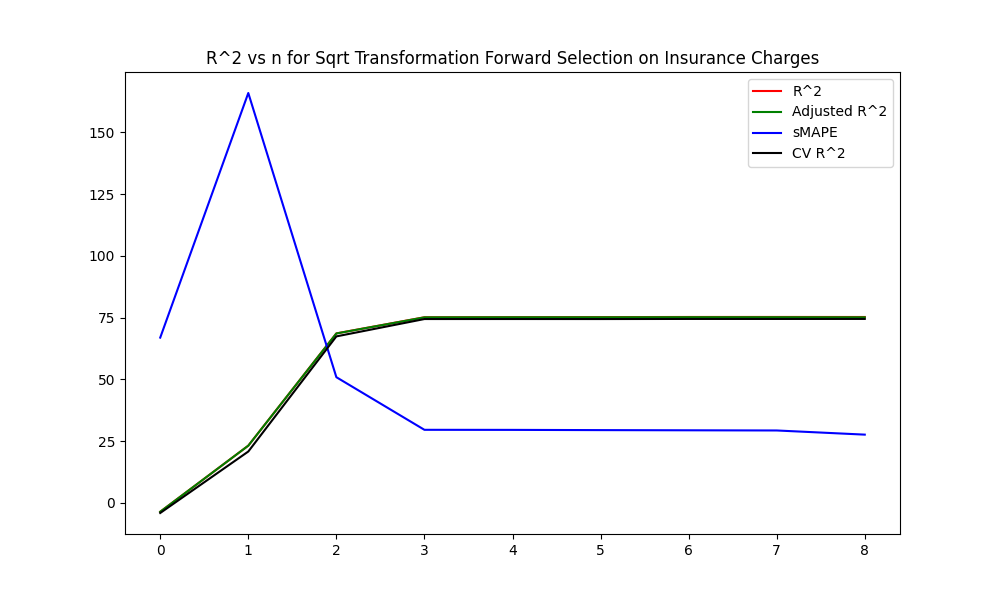
\includegraphics[width=\textwidth]{../Insurance_Charges_Plots/Sqrt_rSq_Forward.png}
     \end{subfigure}
     \hfill
     \begin{subfigure}[b]{0.49\textwidth}
         \centering
         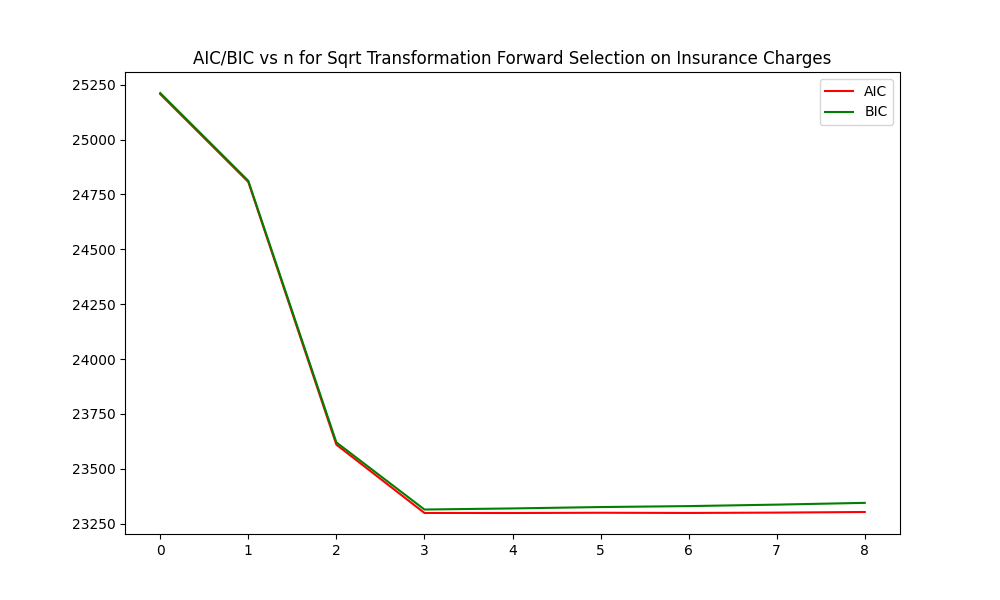
\includegraphics[width=\textwidth]{../Insurance_Charges_Plots/Sqrt_AIC_BIC_Forward.png}
     \end{subfigure}
     
     \caption{Insurance Charges Sqrt Transformation Forward Selection Quality of Fit Metrics\\ Left: $R^2$, Right: AIC/BIC}
     \label{fig:Insurance Charges Sqrt Transformation Forward Selection Quality of Fit Metrics}
\end{figure}

\noindent Backward Elimination Reversed: Null, smoker yes, bmi, age, region southeast, region southwest, region northwest, sex male, children

\begin{figure}[H]
     \centering
     \captionsetup{justification=centering}
     \begin{subfigure}[b]{0.49\textwidth}
         \centering
         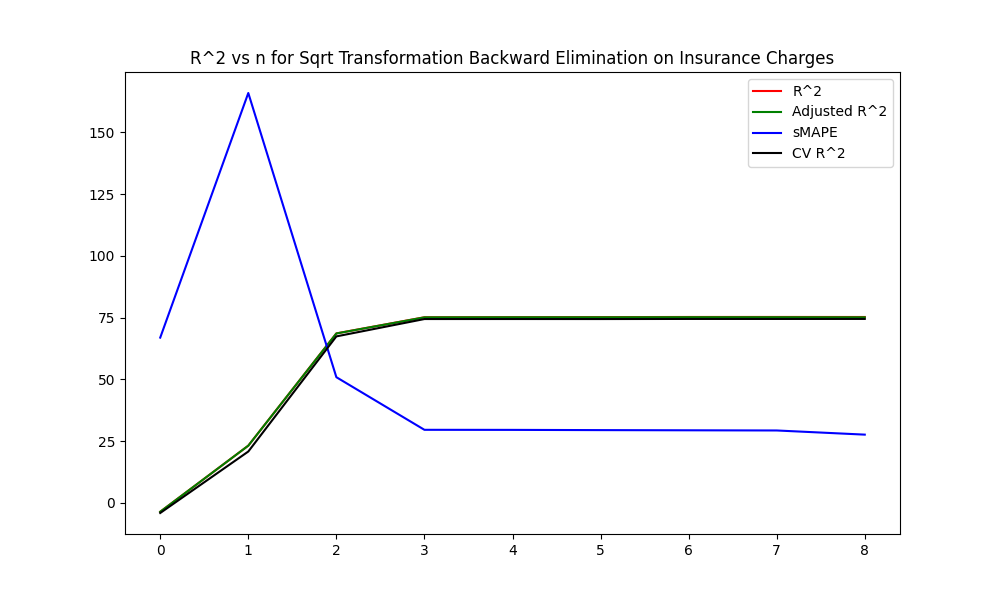
\includegraphics[width=\textwidth]{../Insurance_Charges_Plots/Sqrt_rSq_Backward.png}
     \end{subfigure}
     \hfill
     \begin{subfigure}[b]{0.49\textwidth}
         \centering
         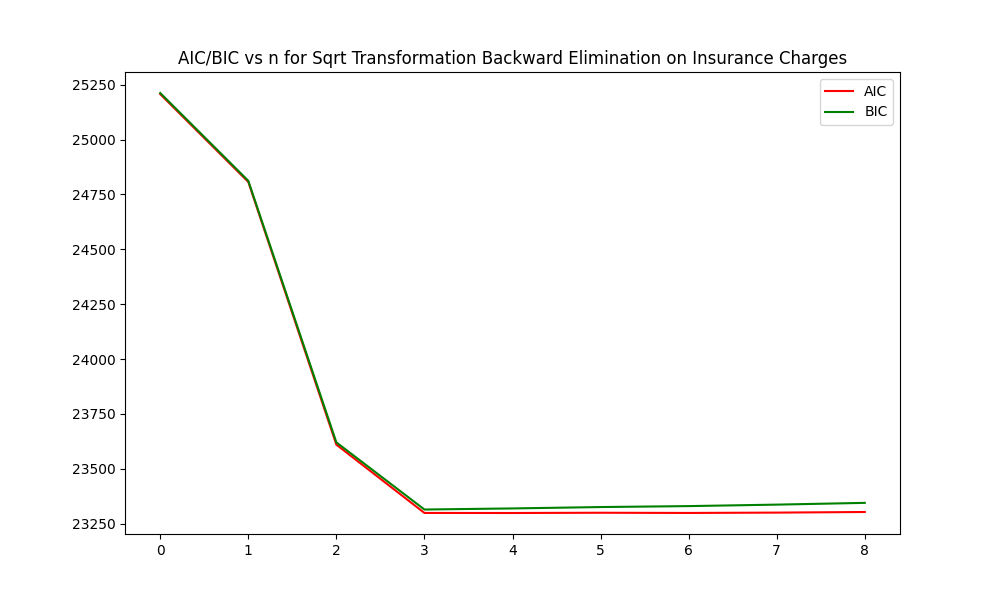
\includegraphics[width=\textwidth]{../Insurance_Charges_Plots/Sqrt_AIC_BIC_Backward.png}
     \end{subfigure}
     
     \caption{Insurance Charges Sqrt Transformation Backward Elimination Quality of Fit Metrics\\ Left: $R^2$, Right: AIC/BIC}
     \label{fig:Insurance Charges Sqrt Transformation Backward Elimination Quality of Fit Metrics}
\end{figure}

\noindent Stepwise Selection: Null, smoker yes, bmi, age, region southeast

\begin{figure}[H]
     \centering
     \captionsetup{justification=centering}
     \begin{subfigure}[b]{0.49\textwidth}
         \centering
         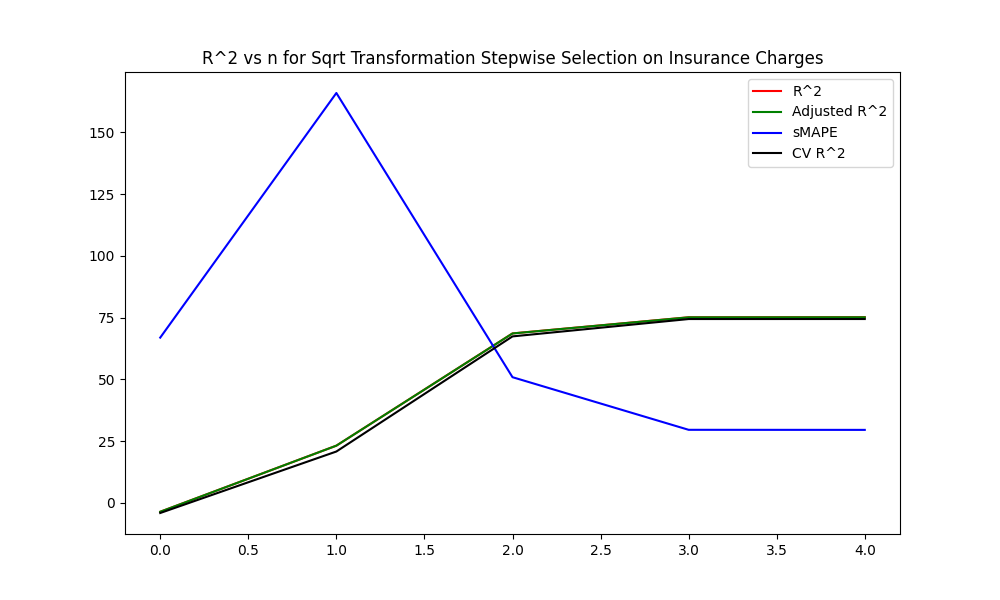
\includegraphics[width=\textwidth]{../Insurance_Charges_Plots/Sqrt_rSq_Stepwise.png}
     \end{subfigure}
     \hfill
     \begin{subfigure}[b]{0.49\textwidth}
         \centering
         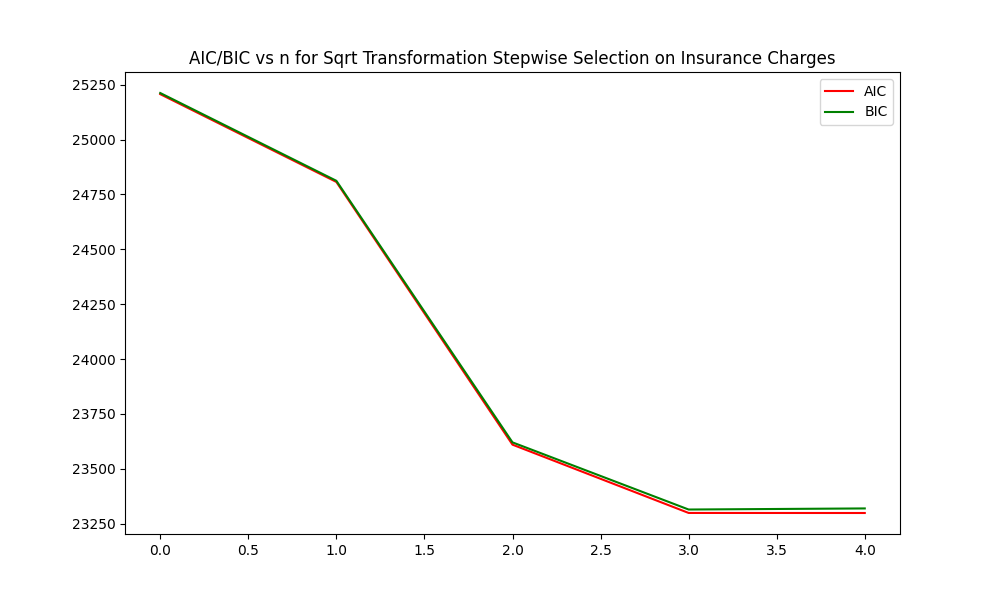
\includegraphics[width=\textwidth]{../Insurance_Charges_Plots/Sqrt_AIC_BIC_Stepwise.png}
     \end{subfigure}
     
     \caption{Insurance Charges Sqrt Transformation Stepwise Selection Quality of Fit Metrics\\ Left: $R^2$, Right: AIC/BIC}
     \label{fig:Insurance Charges Sqrt Transformation Stepwise Selection Quality of Fit Metrics}
\end{figure}

%%%%%%%%%%%%%%%%%%%%%%%%%%%%%%%%%%%%%%%%%%%%%%%%%%%%%%%%%%%%
%%%%%%%%%%%%%%%%%%%%%%%%%%%%%%%%%%%%%%%%%%%%%%%%%%%%%%%%%%%%
%%%%%%%%%%%%%%%%%%%%%%%%%%%%%%%%%%%%%%%%%%%%%%%%%%%%%%%%%%%%
%%%%%%%%%%%%%%%%%%%%%%%%%%%%%%%%%%%%%%%%%%%%%%%%%%%%%%%%%%%%
%%%%%%%%%%%%%%%%%%%%%%%%%%%%%%%%%%%%%%%%%%%%%%%%%%%%%%%%%%%%
%%%%%%%%%%%%%%%%%%%%%%%%%%%%%%%%%%%%%%%%%%%%%%%%%%%%%%%%%%%%

\subsection{Log1p Transformation}

\subsubsection{Quality of Fit}

\begin{figure}[H]
     \centering
     \captionsetup{justification=centering}
     \begin{subfigure}[b]{0.49\textwidth}
         \centering
         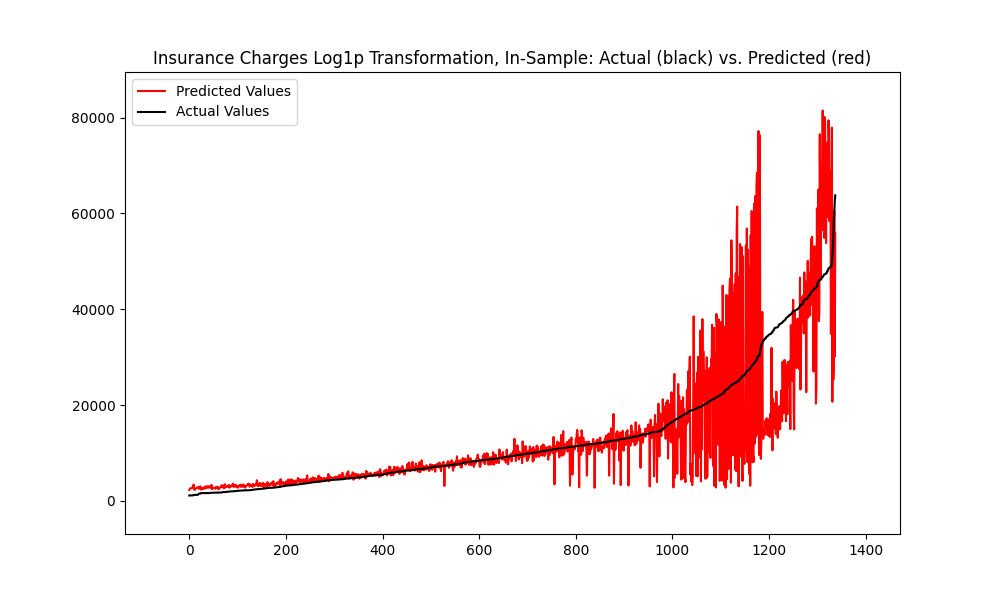
\includegraphics[width=\textwidth]{../Insurance_Charges_Plots/Log1p_In_Sample.png}
     \end{subfigure}
     \hfill
     \begin{subfigure}[b]{0.49\textwidth}
         \centering
         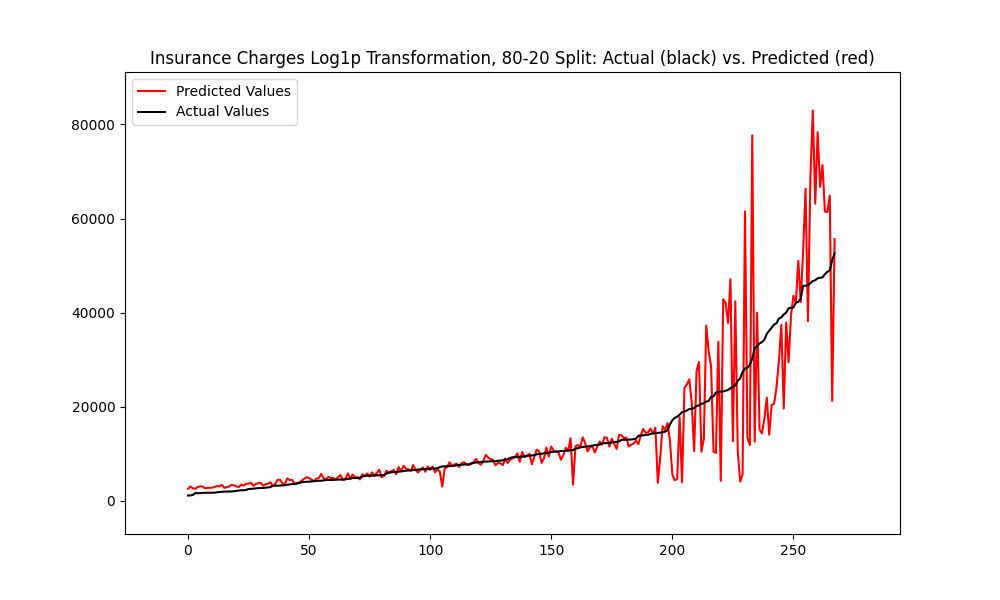
\includegraphics[width=\textwidth]{../Insurance_Charges_Plots/Log1p_80_20.png}
     \end{subfigure}
     
     \caption{Insurance Charges Log1p Transformation Plots\\ Left: In-Sample, Right: Out-of-Sample\\ black: actual y-values, red: predicted y-values}
     \label{fig:Insurance Charges Log1p Transformation Plots}
\end{figure}

\begin{table}[H]
\centering
\caption{Insurance Charges Log1p Transformation}
\label{tab:Insurance Charges Log1p Transformation}
\begin{tabular}{|c|c|c|}\hline
Metric & In-Sample & 80-20 Split \\ \hline \hline
rSq & 0.5228 & 0.5468 \\ \hline
rSqBar & 0.5199 & 0.5328 \\ \hline
sst & 1.961e+11 & 4.265e+10 \\ \hline
sse & 9.357e+10 & 1.933e+10 \\ \hline
sde & 8391 & 8638 \\ \hline
mse0 & 6.993e+07 & 7.211e+07 \\ \hline
rmse & 8363 & 8492 \\ \hline
mae & 4220 & 4213 \\ \hline
smape & 26.29 & 25.08 \\ \hline
m & 1338 & 268 \\ \hline
dfr & 9 & 9 \\ \hline
df & 1329 & 259 \\ \hline
fStat & 161.8 & 34.73 \\ \hline
aic & 2.419e+04 & 4867 \\ \hline
bic & 2.423e+04 & 4899 \\ \hline
\end{tabular}
\end{table}

\begin{table}[H]
\centering
\caption{Insurance Charges Log1p Transformation CV}
\label{tab:Insurance Charges Log1p Transformation CV}
\begin{tabular}{|c|c|c|c|c|c|}\hline
Metric & num folds & min & max & mean & stdev \\ \hline \hline
rSq & 5 & 0.4531 & 0.5468 & 0.5104 & 0.03686 \\ \hline
rSqBar & 5 & 0.4361 & 0.5328 & 0.4953 & 0.03803 \\ \hline
sst & 5 & 2.986e+10 & 4.265e+10 & 3.902e+10 & 4.668e+09 \\ \hline
sse & 5 & 1.395e+10 & 2.294e+10 & 1.915e+10 & 3.002e+09 \\ \hline
sde & 5 & 7339 & 9430 & 8578 & 702.2 \\ \hline
mse0 & 5 & 5.205e+07 & 8.592e+07 & 7.159e+07 & 1.132e+07 \\ \hline
rmse & 5 & 7215 & 9269 & 8433 & 690.1 \\ \hline
mae & 5 & 3509 & 4865 & 4275 & 448.8 \\ \hline
smape & 5 & 25.08 & 28.42 & 26.53 & 1.153 \\ \hline
m & 5 & 267 & 268 & 267.6 & 0.4899 \\ \hline
dfr & 5 & 9 & 9 & 9 & 0 \\ \hline
df & 5 & 258 & 259 & 258.6 & 0.4899 \\ \hline
fStat & 5 & 23.75 & 34.73 & 30.29 & 4.334 \\ \hline
aic & 5 & 4780 & 4896 & 4854 & 39.38 \\ \hline
bic & 5 & 4812 & 4928 & 4887 & 39.37 \\ \hline
\end{tabular}
\end{table}

\subsubsection{Feature Selection}

\noindent Forward Selection: Null, smoker yes, sex male, bmi, age, region northwest, region southwest, children, region southeast

\begin{figure}[H]
     \centering
     \captionsetup{justification=centering}
     \begin{subfigure}[b]{0.49\textwidth}
         \centering
         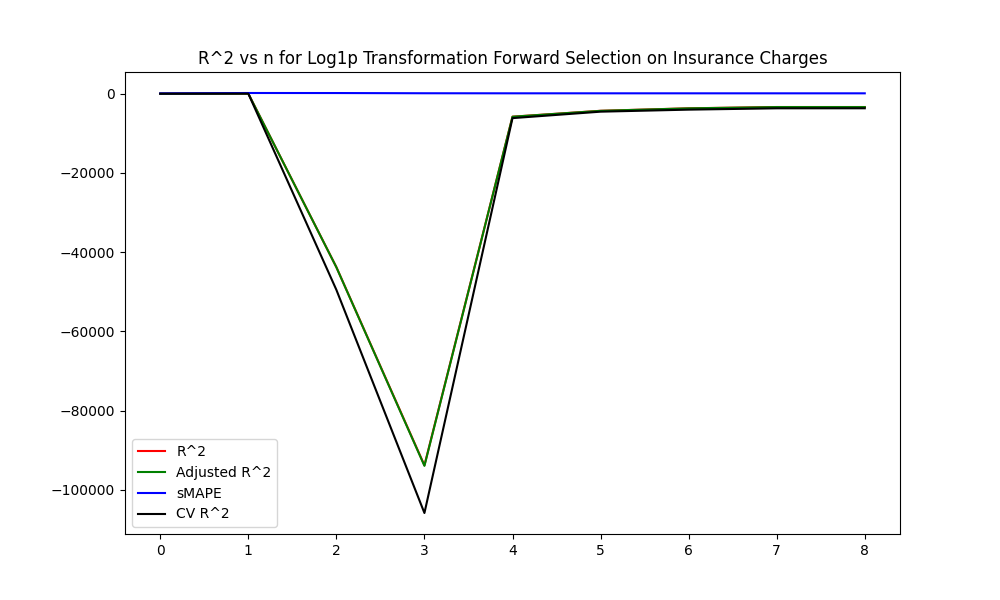
\includegraphics[width=\textwidth]{../Insurance_Charges_Plots/Log1p_rSq_Forward.png}
     \end{subfigure}
     \hfill
     \begin{subfigure}[b]{0.49\textwidth}
         \centering
         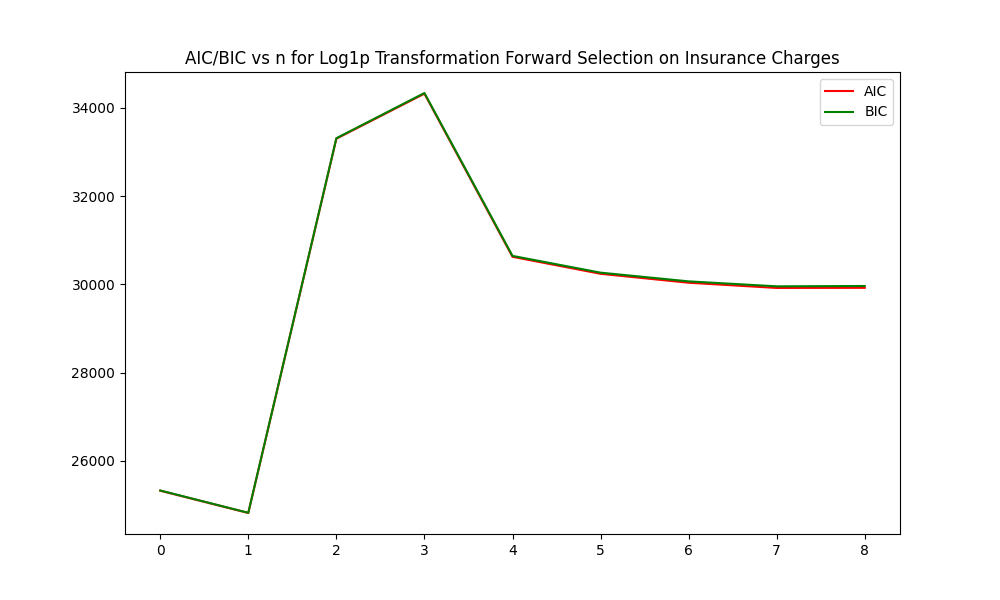
\includegraphics[width=\textwidth]{../Insurance_Charges_Plots/Log1p_AIC_BIC_Forward.png}
     \end{subfigure}
     
     \caption{Insurance Charges Log1p Transformation Forward Selection Quality of Fit Metrics\\ Left: $R^2$, Right: AIC/BIC}
     \label{fig:Insurance Charges Log1p Transformation Forward Selection Quality of Fit Metrics}
\end{figure}

\noindent Backward Elimination Reversed: Null, age, bmi, region northwest, region southwest, sex male, children, region southeast, smoker yes

\begin{figure}[H]
     \centering
     \captionsetup{justification=centering}
     \begin{subfigure}[b]{0.49\textwidth}
         \centering
         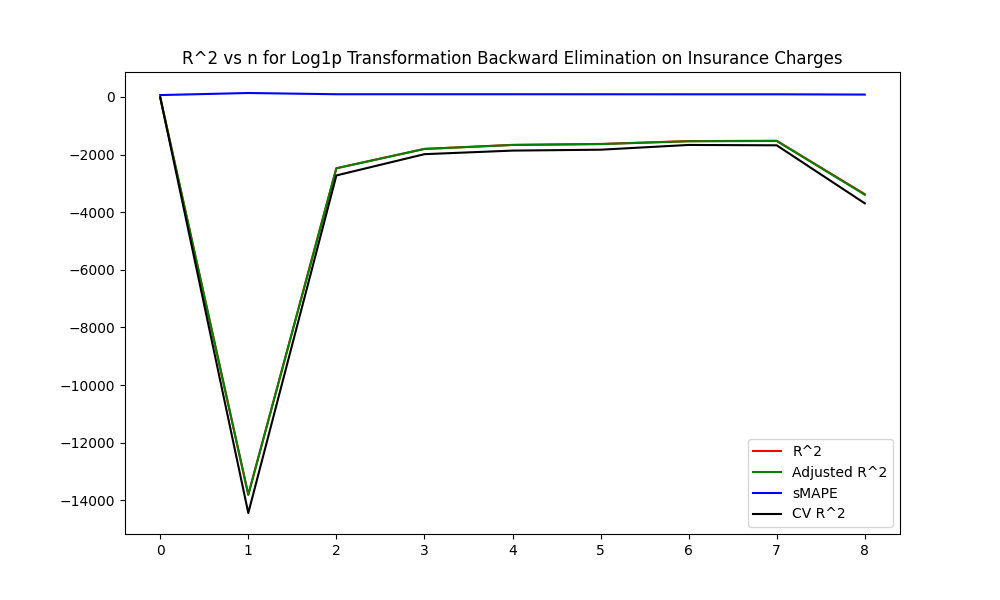
\includegraphics[width=\textwidth]{../Insurance_Charges_Plots/Log1p_rSq_Backward.png}
     \end{subfigure}
     \hfill
     \begin{subfigure}[b]{0.49\textwidth}
         \centering
         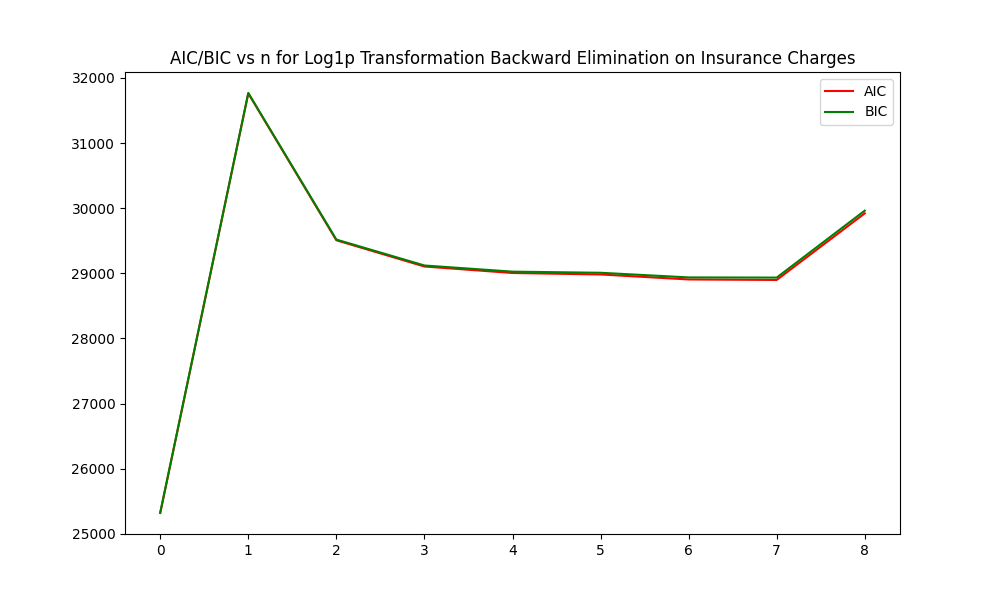
\includegraphics[width=\textwidth]{../Insurance_Charges_Plots/Log1p_AIC_BIC_Backward.png}
     \end{subfigure}
     
     \caption{Insurance Charges Log1p Transformation Backward Elimination Quality of Fit Metrics\\ Left: $R^2$, Right: AIC/BIC}
     \label{fig:Insurance Charges Log1p Transformation Backward Elimination Quality of Fit Metrics}
\end{figure}

\noindent Stepwise Selection: Null, smoker yes

\begin{figure}[H]
     \centering
     \captionsetup{justification=centering}
     \begin{subfigure}[b]{0.49\textwidth}
         \centering
         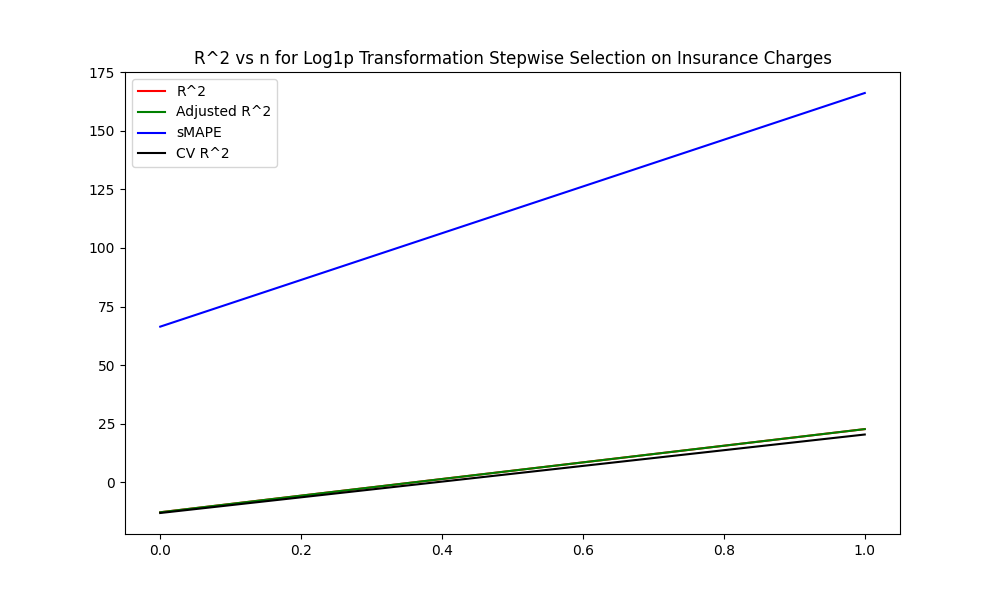
\includegraphics[width=\textwidth]{../Insurance_Charges_Plots/Log1p_rSq_Stepwise.png}
     \end{subfigure}
     \hfill
     \begin{subfigure}[b]{0.49\textwidth}
         \centering
         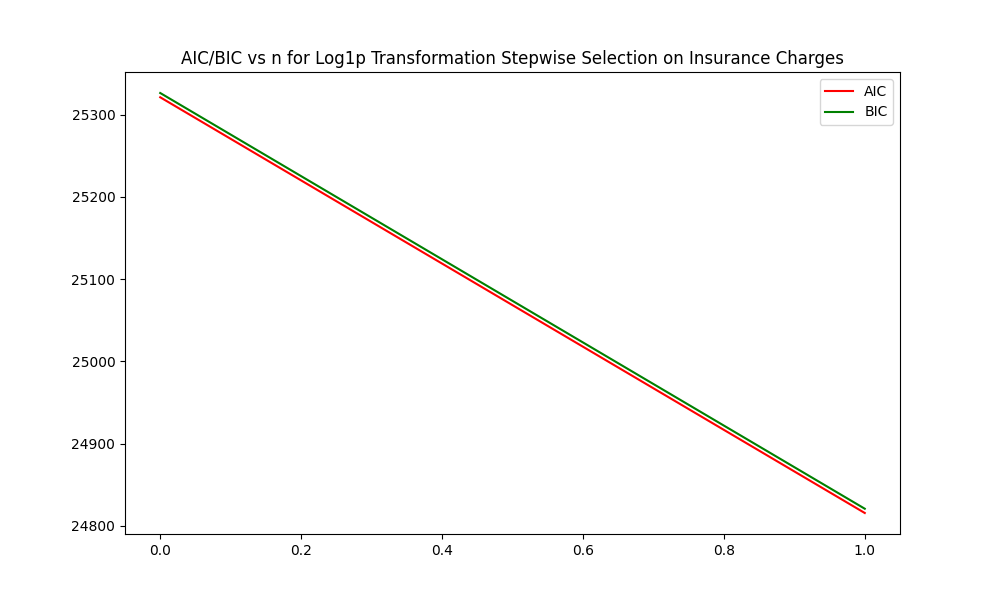
\includegraphics[width=\textwidth]{../Insurance_Charges_Plots/Log1p_AIC_BIC_Stepwise.png}
     \end{subfigure}
     
     \caption{Insurance Charges Log1p Transformation Stepwise Selection Quality of Fit Metrics\\ Left: $R^2$, Right: AIC/BIC}
     \label{fig:Insurance Charges Log1p Transformation Stepwise Selection Quality of Fit Metrics}
\end{figure}

%%%%%%%%%%%%%%%%%%%%%%%%%%%%%%%%%%%%%%%%%%%%%%%%%%%%%%%%%%%%
%%%%%%%%%%%%%%%%%%%%%%%%%%%%%%%%%%%%%%%%%%%%%%%%%%%%%%%%%%%%
%%%%%%%%%%%%%%%%%%%%%%%%%%%%%%%%%%%%%%%%%%%%%%%%%%%%%%%%%%%%
%%%%%%%%%%%%%%%%%%%%%%%%%%%%%%%%%%%%%%%%%%%%%%%%%%%%%%%%%%%%
%%%%%%%%%%%%%%%%%%%%%%%%%%%%%%%%%%%%%%%%%%%%%%%%%%%%%%%%%%%%
%%%%%%%%%%%%%%%%%%%%%%%%%%%%%%%%%%%%%%%%%%%%%%%%%%%%%%%%%%%%

\subsection{Box-Cox Transformation}

\subsubsection{Quality of Fit}

Insurance Charges Box-Cox lambda Used: 0.5

\begin{figure}[H]
     \centering
     \captionsetup{justification=centering}
     \begin{subfigure}[b]{0.49\textwidth}
         \centering
         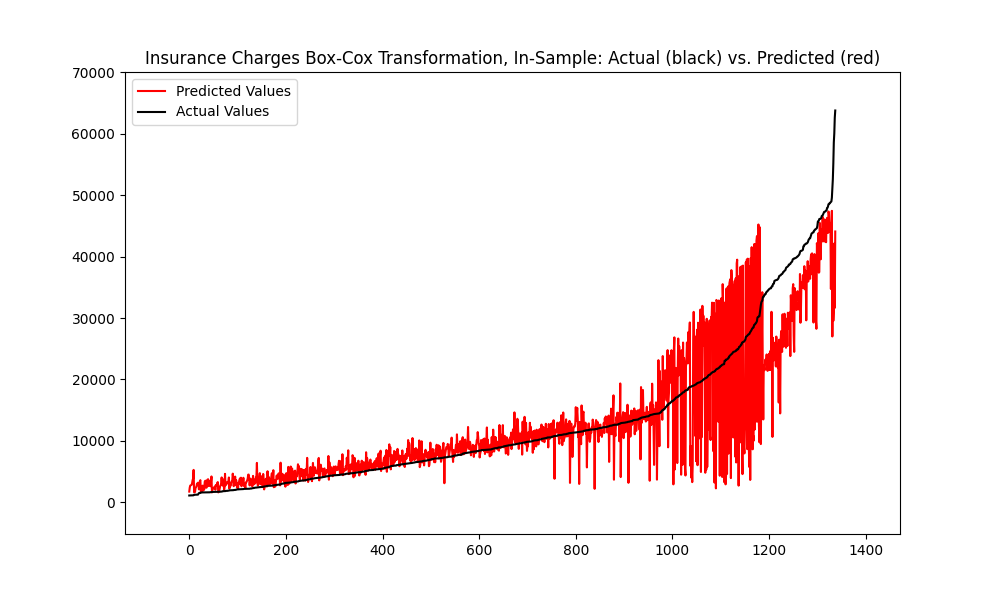
\includegraphics[width=\textwidth]{../Insurance_Charges_Plots/BoxCox_In_Sample.png}
     \end{subfigure}
     \hfill
     \begin{subfigure}[b]{0.49\textwidth}
         \centering
         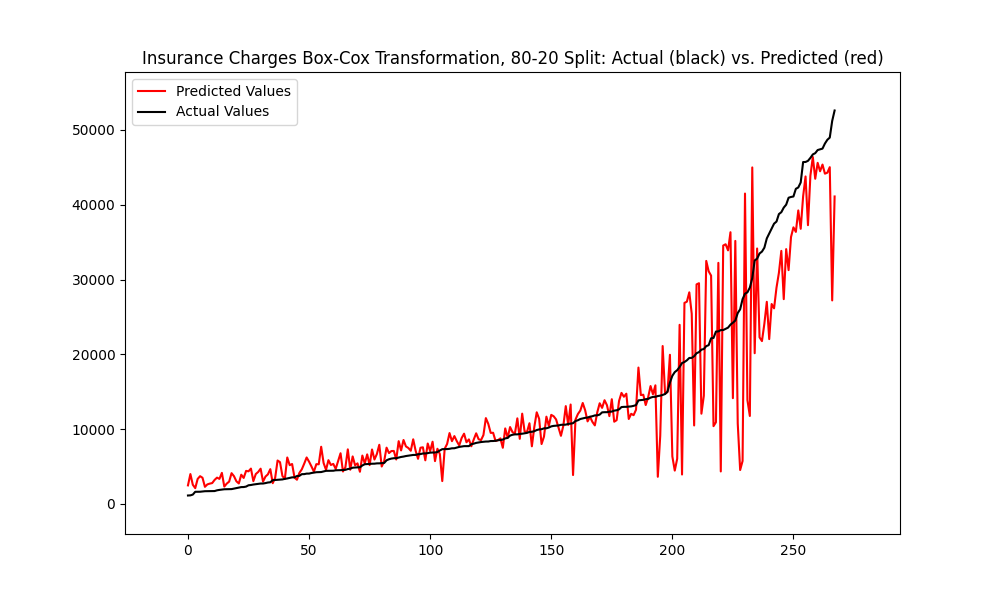
\includegraphics[width=\textwidth]{../Insurance_Charges_Plots/BoxCox_80_20.png}
     \end{subfigure}
     
     \caption{Insurance Charges Box-Cox Transformation Plots\\ Left: In-Sample, Right: Out-of-Sample\\ black: actual y-values, red: predicted y-values}
     \label{fig:Insurance Charges Box-Cox Transformation Plots}
\end{figure}

\begin{table}[H]
\centering
\caption{Insurance Charges Box-Cox Transformation}
\label{tab:Insurance Charges Box-Cox Transformation}
\begin{tabular}{|c|c|c|}\hline
Metric & In-Sample & 80-20 Split \\ \hline \hline
rSq & 0.7527 & 0.8077 \\ \hline
rSqBar & 0.7512 & 0.8017 \\ \hline
sst & 1.961e+11 & 4.265e+10 \\ \hline
sse & 4.85e+10 & 8.202e+09 \\ \hline
sde & 6041 & 5627 \\ \hline
mse0 & 3.625e+07 & 3.06e+07 \\ \hline
rmse & 6020 & 5532 \\ \hline
mae & 3614 & 3316 \\ \hline
smape & 27.69 & 26.47 \\ \hline
m & 1338 & 268 \\ \hline
dfr & 9 & 9 \\ \hline
df & 1329 & 259 \\ \hline
fStat & 449.3 & 120.9 \\ \hline
aic & 2.331e+04 & 4637 \\ \hline
bic & 2.335e+04 & 4670 \\ \hline
\end{tabular}
\end{table}

\begin{table}[H]
\centering
\caption{Insurance Charges Box-Cox Transformation CV}
\label{tab:Insurance Charges Box-Cox Transformation CV}
\begin{tabular}{|c|c|c|c|c|c|}\hline
Metric & num folds & min & max & mean & stdev \\ \hline \hline
rSq & 5 & 0.6982 & 0.8077 & 0.7447 & 0.04001 \\ \hline
rSqBar & 5 & 0.6888 & 0.8017 & 0.7368 & 0.04125 \\ \hline
sst & 5 & 2.986e+10 & 4.265e+10 & 3.902e+10 & 4.668e+09 \\ \hline
sse & 5 & 8.202e+09 & 1.266e+10 & 9.869e+09 & 1.547e+09 \\ \hline
sde & 5 & 5627 & 7005 & 6160 & 476.5 \\ \hline
mse0 & 5 & 3.06e+07 & 4.742e+07 & 3.689e+07 & 5.843e+06 \\ \hline
rmse & 5 & 5532 & 6886 & 6055 & 468.2 \\ \hline
mae & 5 & 3316 & 4146 & 3646 & 299.2 \\ \hline
smape & 5 & 26.47 & 29.49 & 27.88 & 1.068 \\ \hline
m & 5 & 267 & 268 & 267.6 & 0.4899 \\ \hline
dfr & 5 & 9 & 9 & 9 & 0 \\ \hline
df & 5 & 258 & 259 & 258.6 & 0.4899 \\ \hline
fStat & 5 & 66.31 & 120.9 & 86.85 & 19.67 \\ \hline
aic & 5 & 4637 & 4737 & 4677 & 33.57 \\ \hline
bic & 5 & 4670 & 4769 & 4710 & 33.55 \\ \hline
\end{tabular}
\end{table}

\subsubsection{Feature Selection}

\noindent Forward Selection: Null, smoker yes, bmi, age, region southeast, region southwest, region northwest, sex male, children

\begin{figure}[H]
     \centering
     \captionsetup{justification=centering}
     \begin{subfigure}[b]{0.49\textwidth}
         \centering
         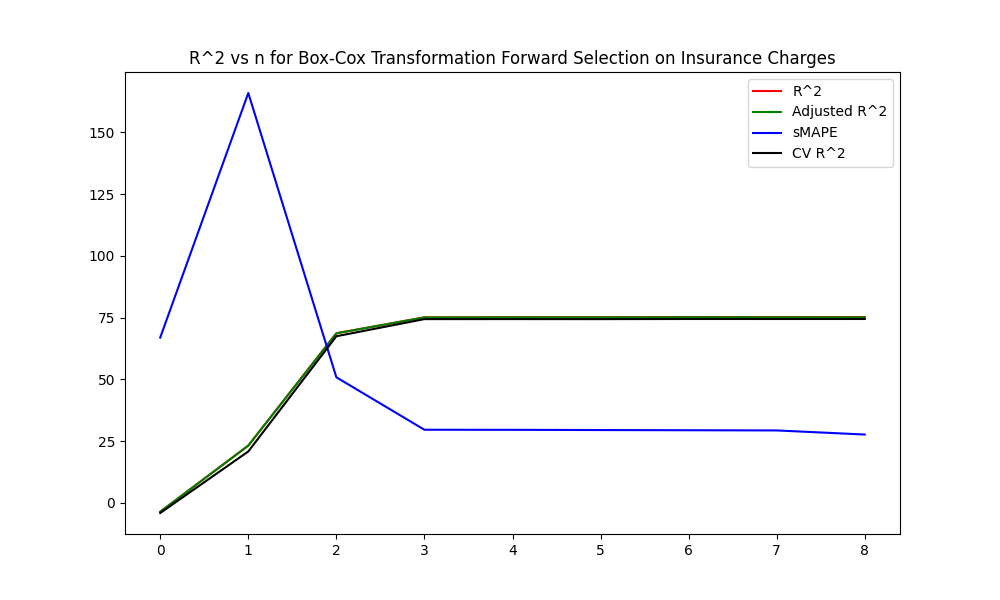
\includegraphics[width=\textwidth]{../Insurance_Charges_Plots/BoxCox_rSq_Forward.png}
     \end{subfigure}
     \hfill
     \begin{subfigure}[b]{0.49\textwidth}
         \centering
         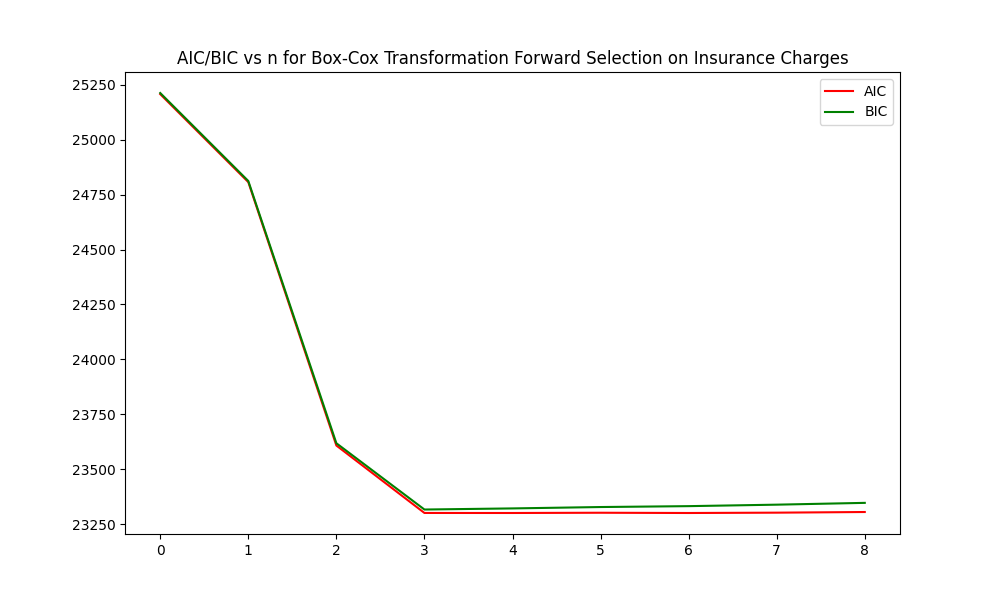
\includegraphics[width=\textwidth]{../Insurance_Charges_Plots/BoxCox_AIC_BIC_Forward.png}
     \end{subfigure}
     
     \caption{Insurance Charges Box-Cox Transformation Forward Selection Quality of Fit Metrics\\ Left: $R^2$, Right: AIC/BIC}
     \label{fig:Insurance Charges Box-Cox Transformation Forward Selection Quality of Fit Metrics}
\end{figure}

\noindent Backward Elimination Reversed: Null, smoker yes, bmi, age, region southeast, region southwest, region northwest, sex male, children

\begin{figure}[H]
     \centering
     \captionsetup{justification=centering}
     \begin{subfigure}[b]{0.49\textwidth}
         \centering
         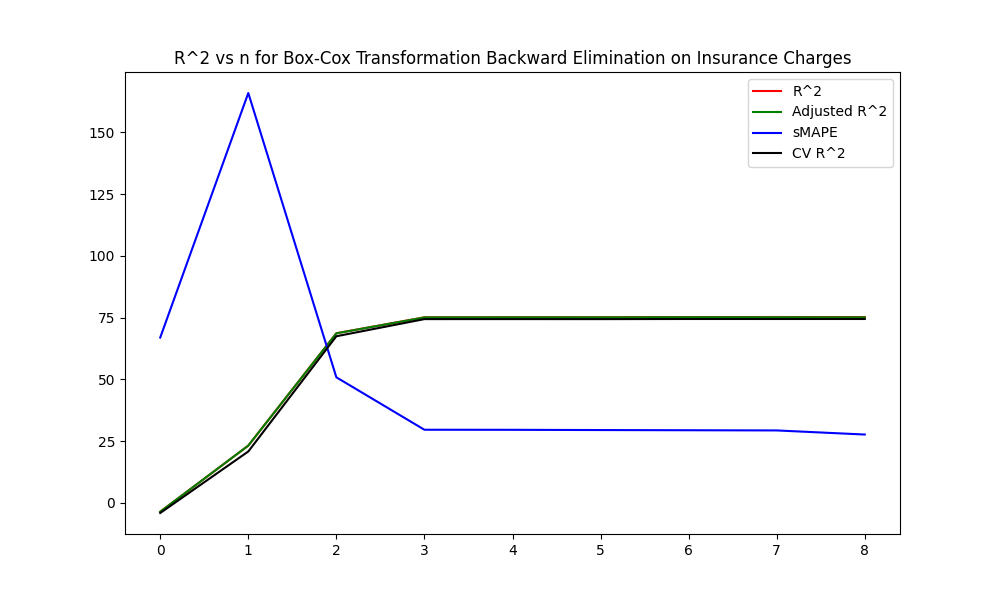
\includegraphics[width=\textwidth]{../Insurance_Charges_Plots/BoxCox_rSq_Backward.png}
     \end{subfigure}
     \hfill
     \begin{subfigure}[b]{0.49\textwidth}
         \centering
         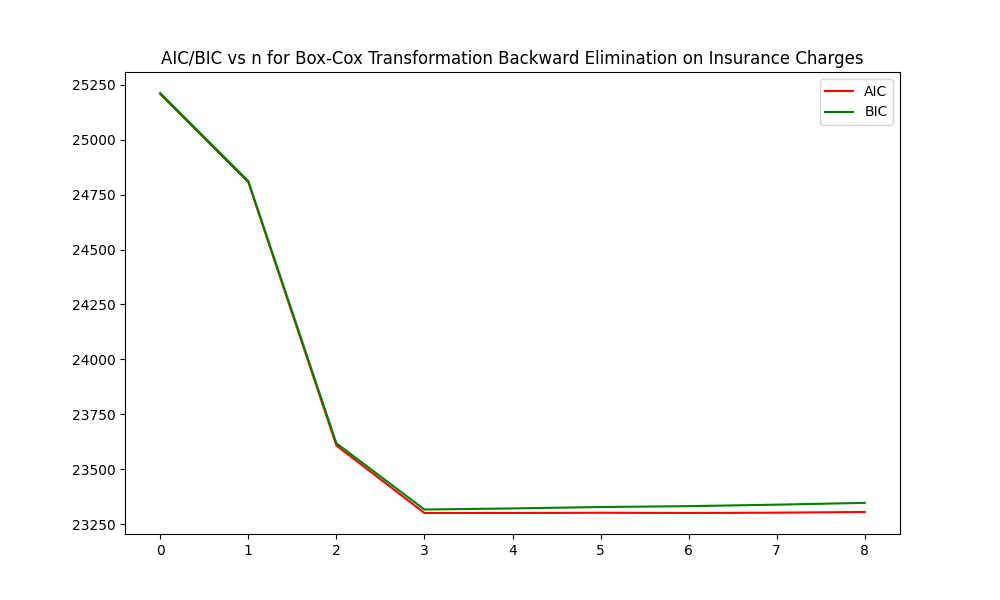
\includegraphics[width=\textwidth]{../Insurance_Charges_Plots/BoxCox_AIC_BIC_Backward.png}
     \end{subfigure}
     
     \caption{Insurance Charges Box-Cox Transformation Backward Elimination Quality of Fit Metrics\\ Left: $R^2$, Right: AIC/BIC}
     \label{fig:Insurance Charges Box-Cox Transformation Backward Elimination Quality of Fit Metrics}
\end{figure}

\noindent Stepwise Selection: Null, smoker yes, bmi, age, region southeast

\begin{figure}[H]
     \centering
     \captionsetup{justification=centering}
     \begin{subfigure}[b]{0.49\textwidth}
         \centering
         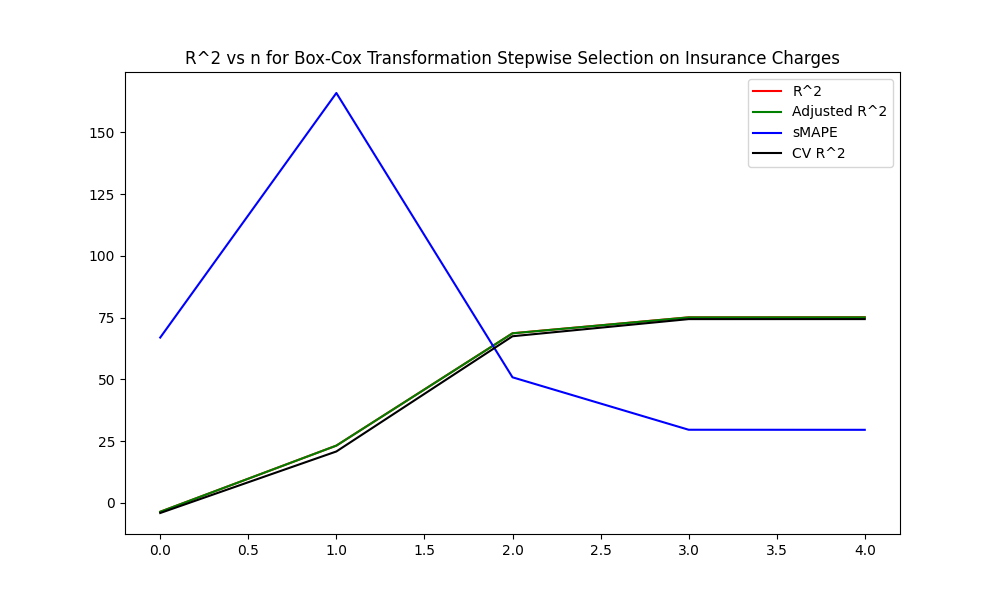
\includegraphics[width=\textwidth]{../Insurance_Charges_Plots/BoxCox_rSq_Stepwise.png}
     \end{subfigure}
     \hfill
     \begin{subfigure}[b]{0.49\textwidth}
         \centering
         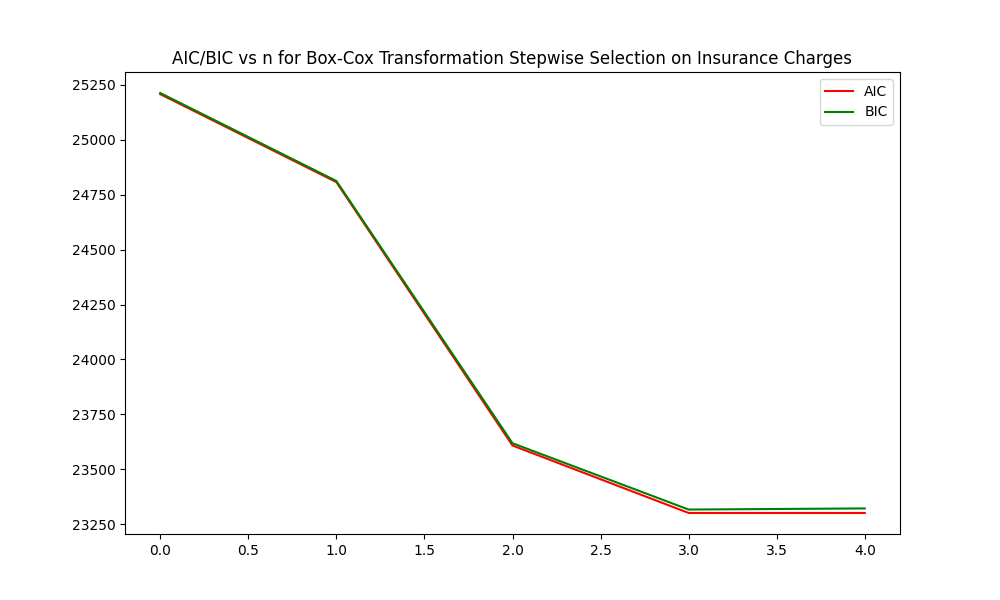
\includegraphics[width=\textwidth]{../Insurance_Charges_Plots/BoxCox_AIC_BIC_Stepwise.png}
     \end{subfigure}
     
     \caption{Insurance Charges Box-Cox Transformation Stepwise Selection Quality of Fit Metrics\\ Left: $R^2$, Right: AIC/BIC}
     \label{fig:Insurance Charges Box-Cox Transformation Stepwise Selection Quality of Fit Metrics}
\end{figure}

%%%%%%%%%%%%%%%%%%%%%%%%%%%%%%%%%%%%%%%%%%%%%%%%%%%%%%%%%%%%
%%%%%%%%%%%%%%%%%%%%%%%%%%%%%%%%%%%%%%%%%%%%%%%%%%%%%%%%%%%%
%%%%%%%%%%%%%%%%%%%%%%%%%%%%%%%%%%%%%%%%%%%%%%%%%%%%%%%%%%%%
%%%%%%%%%%%%%%%%%%%%%%%%%%%%%%%%%%%%%%%%%%%%%%%%%%%%%%%%%%%%
%%%%%%%%%%%%%%%%%%%%%%%%%%%%%%%%%%%%%%%%%%%%%%%%%%%%%%%%%%%%
%%%%%%%%%%%%%%%%%%%%%%%%%%%%%%%%%%%%%%%%%%%%%%%%%%%%%%%%%%%%

\subsection{Order 2 Regression}

\subsubsection{Quality of Fit}

Insurance Charges Order 2 Polynomial alpha Used: 0.0008500000000000002

\begin{figure}[H]
     \centering
     \captionsetup{justification=centering}
     \begin{subfigure}[b]{0.49\textwidth}
         \centering
         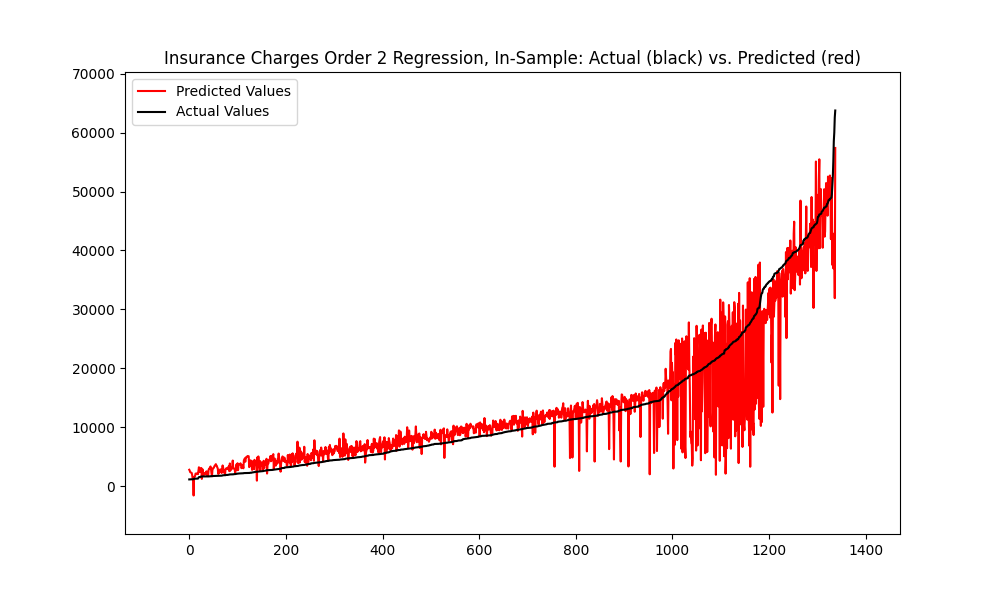
\includegraphics[width=\textwidth]{../Insurance_Charges_Plots/Order2Reg_In_Sample.png}
     \end{subfigure}
     \hfill
     \begin{subfigure}[b]{0.49\textwidth}
         \centering
         
\includegraphics[width=\textwidth]{../Insurance_Charges_Plots/Order2Reg_80_20.png}
     \end{subfigure}
     
     \caption{Insurance Charges Order 2 Regression Plots\\ Left: In-Sample, Right: Out-of-Sample\\ black: actual y-values, red: predicted y-values}
     \label{fig:Insurance Charges Order 2 Regression Plots}
\end{figure}

\begin{table}[H]
\centering
\caption{Insurance Charges Order 2 Polynomial Regression}
\label{tab:Insurance Charges Order 2 Polynomial Regression}
\begin{tabular}{|c|c|c|}\hline
Metric & In-Sample & 80-20 Split \\ \hline \hline
rSq & 0.8477 & 0.88 \\ \hline
rSqBar & 0.8406 & 0.8452 \\ \hline
sst & 1.961e+11 & 4.265e+10 \\ \hline
sse & 2.986e+10 & 5.117e+09 \\ \hline
sde & 4835 & 4972 \\ \hline
mse0 & 2.232e+07 & 1.909e+07 \\ \hline
rmse & 4724 & 4370 \\ \hline
mae & 2833 & 2957 \\ \hline
smape & 26.43 & 28.54 \\ \hline
m & 1338 & 268 \\ \hline
dfr & 61 & 61 \\ \hline
df & 1277 & 207 \\ \hline
fStat & 116.5 & 24.89 \\ \hline
aic & 2.276e+04 & 4615 \\ \hline
bic & 2.308e+04 & 4834 \\ \hline
\end{tabular}
\end{table}

\begin{table}[H]
\centering
\caption{Insurance Charges Order 2 Polynomial Regression CV}
\label{tab:Insurance Charges Order 2 Polynomial Regression CV}
\begin{tabular}{|c|c|c|c|c|c|}\hline
Metric & num folds & min & max & mean & stdev \\ \hline \hline
rSq & 5 & 0.7851 & 0.88 & 0.836 & 0.0399 \\ \hline
rSqBar & 5 & 0.7225 & 0.8452 & 0.7884 & 0.05152 \\ \hline
sst & 5 & 2.986e+10 & 4.265e+10 & 3.902e+10 & 4.668e+09 \\ \hline
sse & 5 & 5.117e+09 & 9.015e+09 & 6.302e+09 & 1.412e+09 \\ \hline
sde & 5 & 4972 & 6615 & 5492 & 590.4 \\ \hline
mse0 & 5 & 1.909e+07 & 3.377e+07 & 2.356e+07 & 5.312e+06 \\ \hline
rmse & 5 & 4370 & 5811 & 4826 & 517.8 \\ \hline
mae & 5 & 2616 & 3289 & 2913 & 220.3 \\ \hline
smape & 5 & 25.79 & 28.54 & 26.99 & 0.9621 \\ \hline
m & 5 & 267 & 268 & 267.6 & 0.4899 \\ \hline
dfr & 5 & 61 & 61 & 61 & 0 \\ \hline
df & 5 & 206 & 207 & 206.6 & 0.4899 \\ \hline
fStat & 5 & 12.34 & 24.89 & 18.49 & 5.052 \\ \hline
aic & 5 & 4615 & 4750 & 4658 & 49.31 \\ \hline
bic & 5 & 4834 & 4969 & 4877 & 49.25 \\ \hline
\end{tabular}
\end{table}

\subsubsection{Feature Selection}

\noindent Forward Selection: Null, bmi x smoker yes, age x age, smoker no, children x smoker no, bmi x region northeast, children x region northwest, age x region northeast, children x sex female, smoker yes x region southwest, children x region southwest, smoker yes x region southeast, sex male x region northeast, age x region northwest, bmi x region northwest, bmi x bmi, bmi, children, children x children, region northwest, sex male x region southwest, age x children, bmi x smoker no, children x region northeast, age x region southwest, bmi x region southwest, smoker no x region southeast, age x sex female, sex female, sex male x region northwest, smoker no x region northwest, smoker yes, smoker no x region northeast, age x smoker yes, age, age x bmi, bmi x sex male, bmi x children, sex male x smoker yes, sex female x smoker yes, bmi x sex female, sex female x smoker no, sex male x smoker no, smoker yes x region northwest, smoker yes x region northeast, children x sex male, age x smoker no, smoker no x region southwest, children x region southeast, sex female x region northeast, sex male, region southwest, sex female x region southwest, sex male x region southeast, region northeast, sex female x region northwest, sex female x region southeast, region southeast, children x smoker yes, age x sex male, age x region southeast, bmi x region southeast

\begin{figure}[H]
     \centering
     \captionsetup{justification=centering}
     \begin{subfigure}[b]{0.49\textwidth}
         \centering
         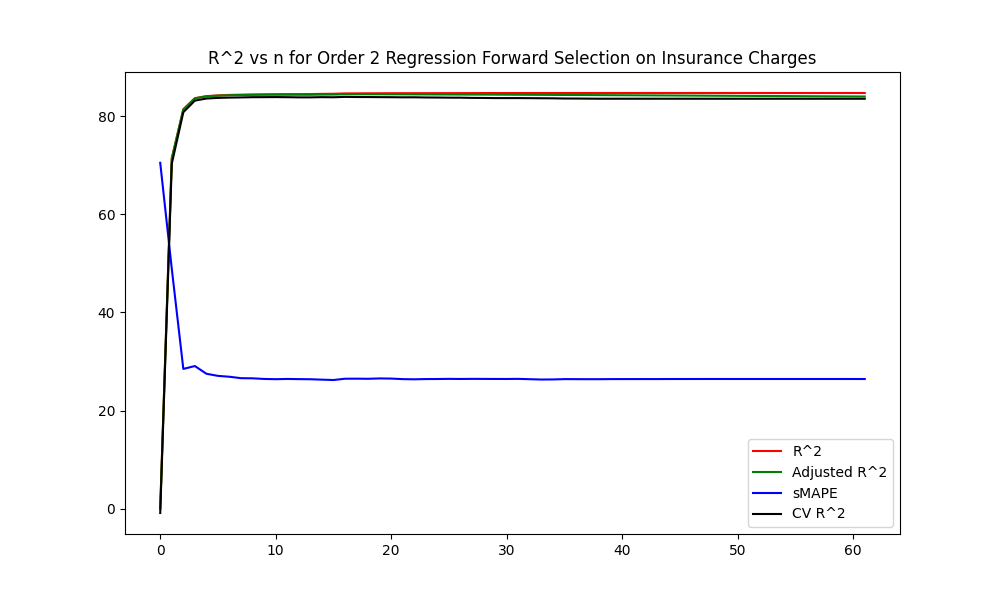
\includegraphics[width=\textwidth]{../Insurance_Charges_Plots/Order2Reg_rSq_Forward.png}
     \end{subfigure}
     \hfill
     \begin{subfigure}[b]{0.49\textwidth}
         \centering
         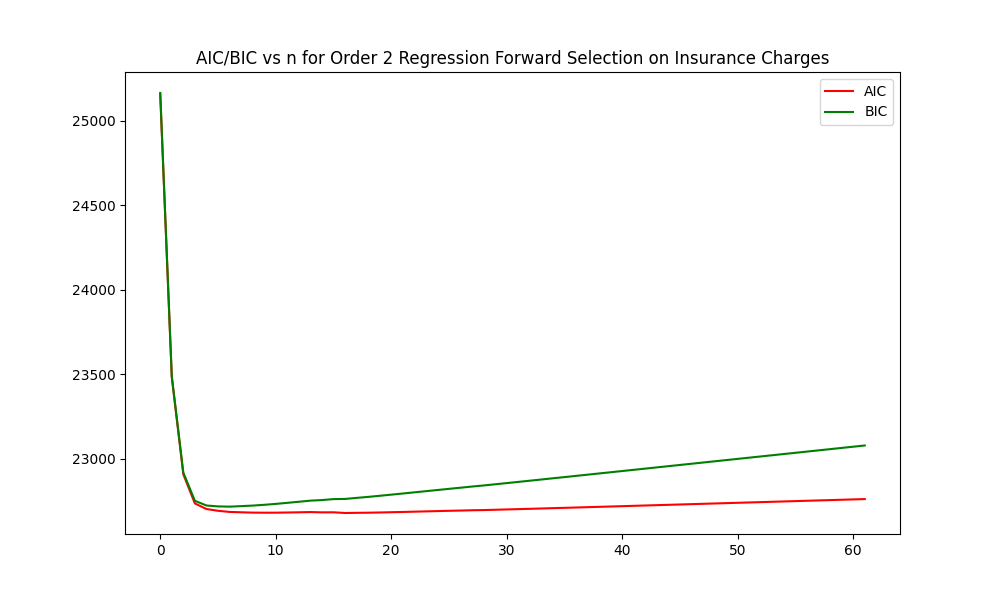
\includegraphics[width=\textwidth]{../Insurance_Charges_Plots/Order2Reg_AIC_BIC_Forward.png}
     \end{subfigure}
     
     \caption{Insurance Charges Order 2 Regression Forward Selection Quality of Fit Metrics\\ Left: $R^2$, Right: AIC/BIC}
     \label{fig:Insurance Charges Order 2 Regression Forward Selection Quality of Fit Metrics}
\end{figure}

\noindent Backward Elimination Reversed: Null, bmi x smoker yes, age x age, smoker yes, children x smoker no, bmi x region northeast, bmi x bmi, bmi, children x region northwest, children x sex female, age x region northeast, age x region northwest, bmi x region northwest, smoker yes x region southwest, smoker no x region southeast, children x region northeast, sex female x smoker no, sex male x smoker yes, age x sex female, children x children, children x region southeast, bmi x region southwest, sex female x region northeast, smoker yes x region southeast, children, bmi x smoker no, age x children, sex male x region southwest, sex male x region northwest, age, age x bmi, smoker yes x region northwest, smoker no, smoker no x region southwest, smoker no x region northeast, age x region southeast, age x smoker yes, sex female x smoker yes, bmi x children, bmi x sex male, smoker yes x region northeast, bmi x sex female, sex male x smoker no, age x smoker no, children x sex male, sex male, smoker no x region northwest, sex female, region northwest, region southwest, sex female x region southwest, sex male x region southeast, sex female x region northwest, sex male x region northeast, region northeast, sex female x region southeast, region southeast, children x smoker yes, children x region southwest, age x sex male, age x region southwest, bmi x region southeast

\begin{figure}[H]
     \centering
     \captionsetup{justification=centering}
     \begin{subfigure}[b]{0.49\textwidth}
         \centering
         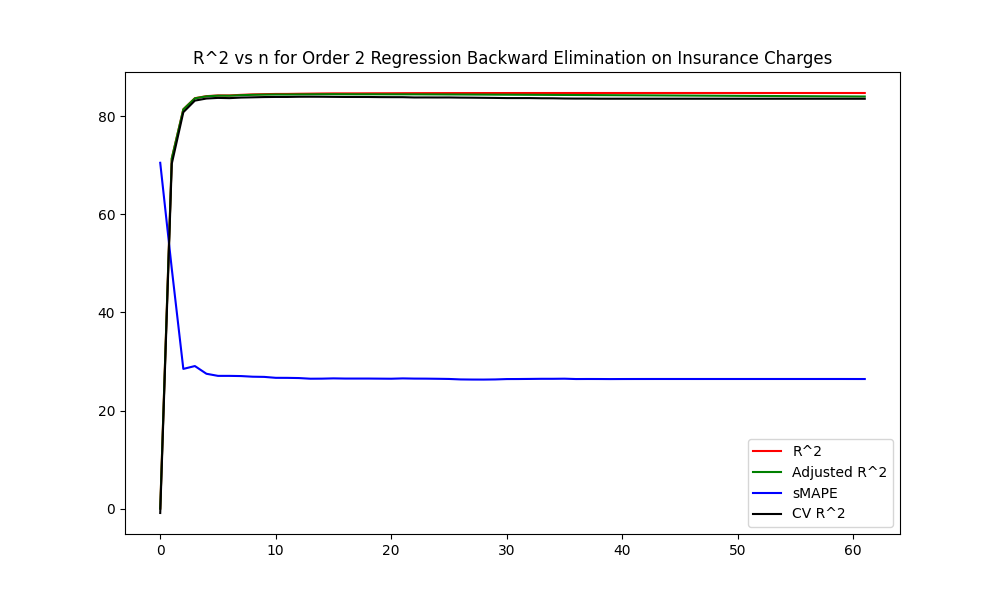
\includegraphics[width=\textwidth]{../Insurance_Charges_Plots/Order2Reg_rSq_Backward.png}
     \end{subfigure}
     \hfill
     \begin{subfigure}[b]{0.49\textwidth}
         \centering
         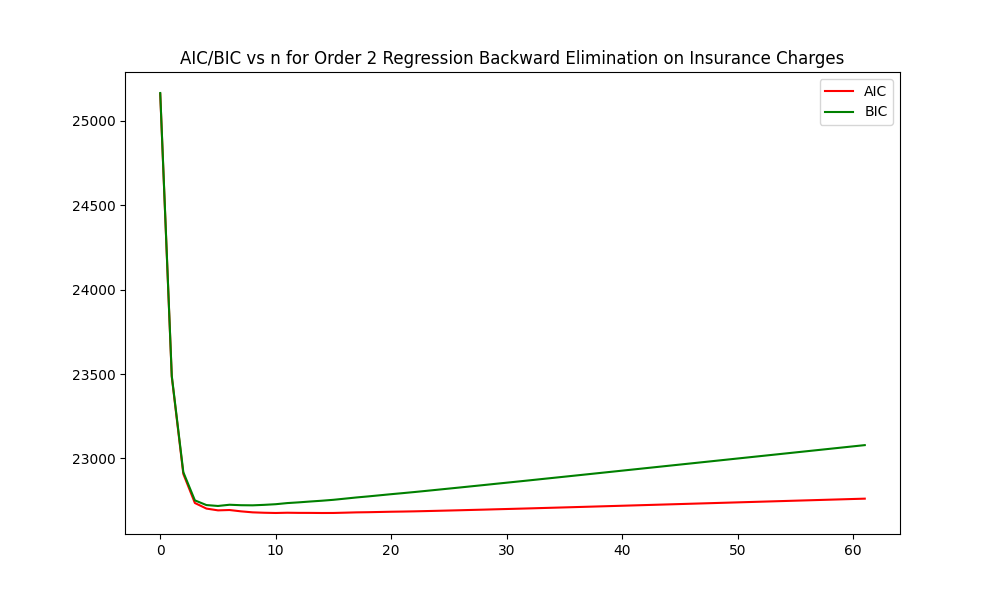
\includegraphics[width=\textwidth]{../Insurance_Charges_Plots/Order2Reg_AIC_BIC_Backward.png}
     \end{subfigure}
     
     \caption{Insurance Charges Order 2 Regression Backward Elimination Quality of Fit Metrics\\ Left: $R^2$, Right: AIC/BIC}
     \label{fig:Insurance Charges Order 2 Regression Backward Elimination Quality of Fit Metrics}
\end{figure}

\noindent Stepwise Selection: Null, bmi x smoker yes, age x age, smoker no, children x smoker no, bmi x region northeast, children x region northwest, age x region northeast, children x sex female, smoker yes x region southwest, children x region southwest

\begin{figure}[H]
     \centering
     \captionsetup{justification=centering}
     \begin{subfigure}[b]{0.49\textwidth}
         \centering
         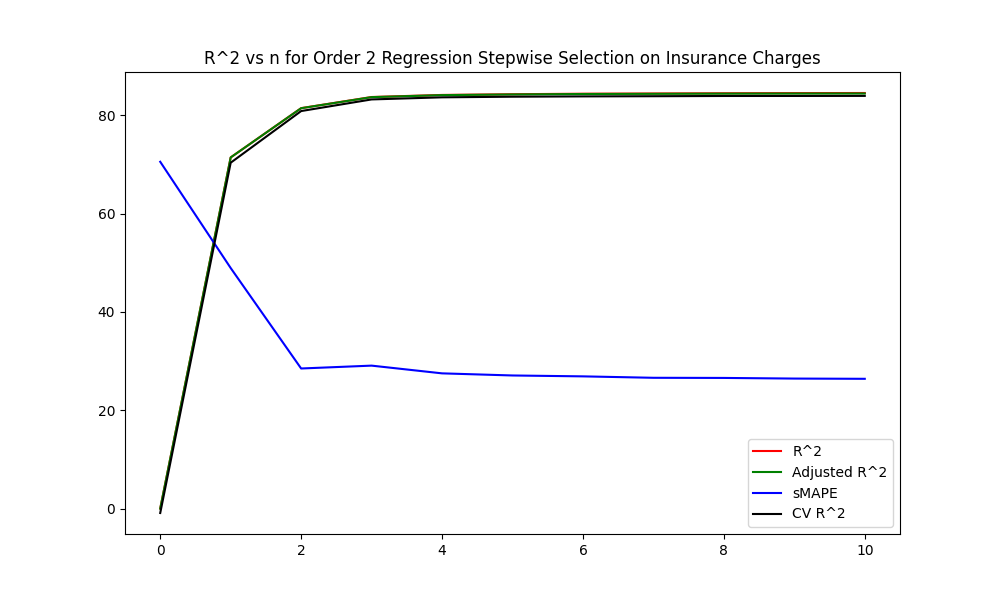
\includegraphics[width=\textwidth]{../Insurance_Charges_Plots/Order2Reg_rSq_Stepwise.png}
     \end{subfigure}
     \hfill
     \begin{subfigure}[b]{0.49\textwidth}
         \centering
         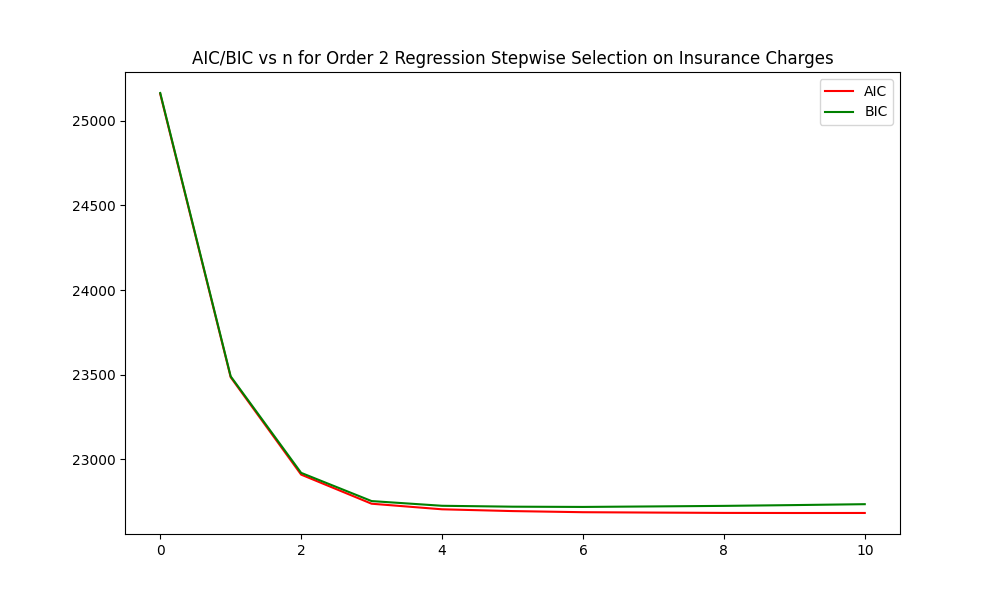
\includegraphics[width=\textwidth]{../Insurance_Charges_Plots/Order2Reg_AIC_BIC_Stepwise.png}
     \end{subfigure}
     
     \caption{Insurance Charges Order 2 Regression Stepwise Selection Quality of Fit Metrics\\ Left: $R^2$, Right: AIC/BIC}
     \label{fig:Insurance Charges Order 2 Regression Stepwise Selection Quality of Fit Metrics}
\end{figure}

%%%%%%%%%%%%%%%%%%%%%%%%%%%%%%%%%%%%%%%%%%%%%%%%%%%%%%%%%%%%
%%%%%%%%%%%%%%%%%%%%%%%%%%%%%%%%%%%%%%%%%%%%%%%%%%%%%%%%%%%%
%%%%%%%%%%%%%%%%%%%%%%%%%%%%%%%%%%%%%%%%%%%%%%%%%%%%%%%%%%%%
%%%%%%%%%%%%%%%%%%%%%%%%%%%%%%%%%%%%%%%%%%%%%%%%%%%%%%%%%%%%
%%%%%%%%%%%%%%%%%%%%%%%%%%%%%%%%%%%%%%%%%%%%%%%%%%%%%%%%%%%%
%%%%%%%%%%%%%%%%%%%%%%%%%%%%%%%%%%%%%%%%%%%%%%%%%%%%%%%%%%%%

\subsection{Two Layer Neural Network}

\subsubsection{Quality of Fit}

Insurance Charges NN 2L output activation: ELU, lr: 5e-03

\begin{figure}[H]
     \centering
     \captionsetup{justification=centering}
     \begin{subfigure}[b]{0.49\textwidth}
         \centering
         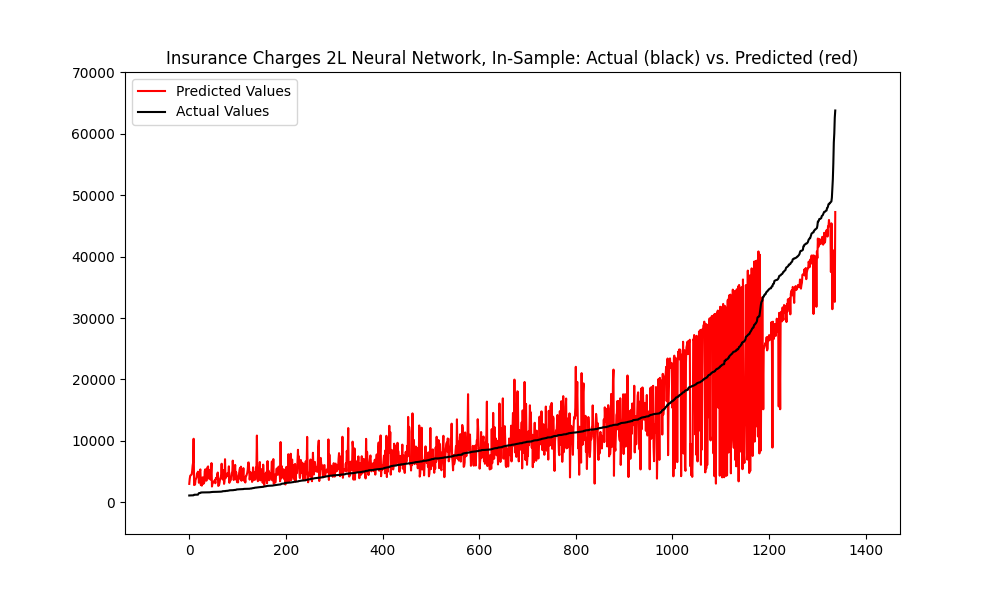
\includegraphics[width=\textwidth]{../Insurance_Charges_Plots/NN_2L_In_Sample.png}
     \end{subfigure}
     \hfill
     \begin{subfigure}[b]{0.49\textwidth}
         \centering
         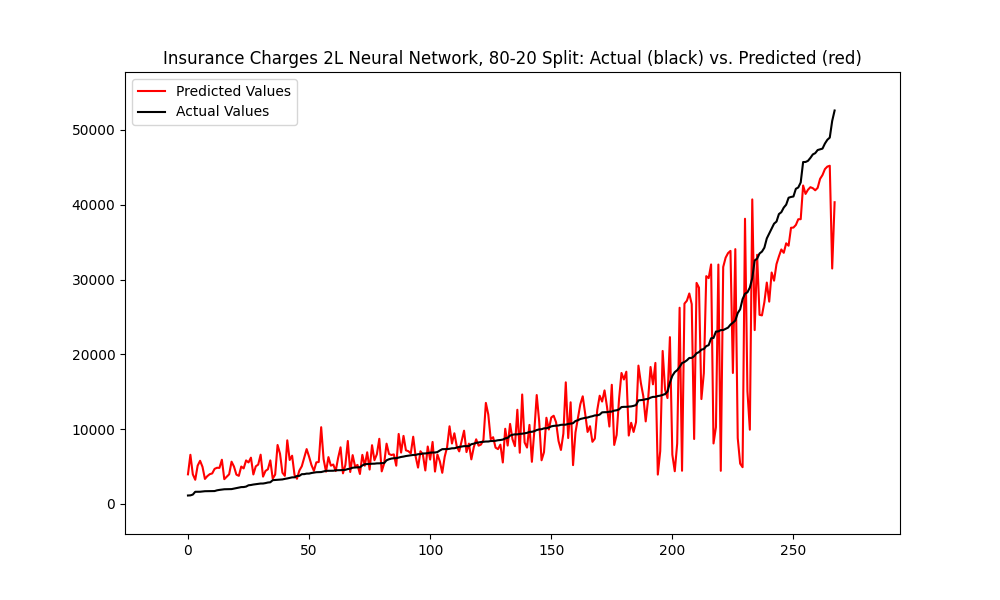
\includegraphics[width=\textwidth]{../Insurance_Charges_Plots/NN_2L_80_20.png}
     \end{subfigure}
     
     \caption{Insurance Charges 2 Layer Neural Network Plots\\ Left: In-Sample, Right: Out-of-Sample\\ black: actual y-values, red: predicted y-values}
     \label{fig:Insurance Charges 2 Layer Neural Network Plots}
\end{figure}

\begin{table}[H]
\centering
\caption{Insurance Charges 2L Neural Network}
\label{tab:Insurance Charges 2L Neural Network}
\begin{tabular}{|c|c|c|}\hline
Metric & In-Sample & 80-20 Split \\ \hline \hline
rSq & 0.7703 & 0.8211 \\ \hline
rSqBar & 0.7691 & 0.8163 \\ \hline
sst & 1.961e+11 & 4.265e+10 \\ \hline
sse & 4.504e+10 & 7.631e+09 \\ \hline
sde & 5819 & 5418 \\ \hline
mse0 & 3.366e+07 & 2.847e+07 \\ \hline
rmse & 5802 & 5336 \\ \hline
mae & 3996 & 3668 \\ \hline
smape & 35.78 & 33.65 \\ \hline
m & 1338 & 268 \\ \hline
dfr & 8 & 8 \\ \hline
df & 1330 & 260 \\ \hline
fStat & 557.5 & 149.1 \\ \hline
aic & 2.321e+04 & 4616 \\ \hline
bic & 2.325e+04 & 4645 \\ \hline
\end{tabular}
\end{table}

\begin{table}[H]
\centering
\caption{Insurance Charges 2L Neural Network CV}
\label{tab:Insurance Charges 2L Neural Network CV}
\begin{tabular}{|c|c|c|c|c|c|}\hline
Metric & num folds & min & max & mean & stdev \\ \hline \hline
rSq & 5 & 0.6721 & 0.8208 & 0.7589 & 0.05256 \\ \hline
rSqBar & 5 & 0.6632 & 0.816 & 0.7524 & 0.05397 \\ \hline
sst & 5 & 2.986e+10 & 4.265e+10 & 3.902e+10 & 4.668e+09 \\ \hline
sse & 5 & 7.643e+09 & 1.13e+10 & 9.209e+09 & 1.279e+09 \\ \hline
sde & 5 & 5422 & 6604 & 5942 & 413.2 \\ \hline
mse0 & 5 & 2.852e+07 & 4.231e+07 & 3.442e+07 & 4.822e+06 \\ \hline
rmse & 5 & 5340 & 6505 & 5852 & 406.8 \\ \hline
mae & 5 & 3668 & 4449 & 4045 & 256.5 \\ \hline
smape & 5 & 33.62 & 39.57 & 36.06 & 2.255 \\ \hline
m & 5 & 267 & 268 & 267.6 & 0.4899 \\ \hline
dfr & 5 & 8 & 8 & 8 & 0 \\ \hline
df & 5 & 259 & 260 & 259.6 & 0.4899 \\ \hline
fStat & 5 & 66.6 & 148.9 & 108.3 & 28.85 \\ \hline
aic & 5 & 4616 & 4705 & 4657 & 32.09 \\ \hline
bic & 5 & 4645 & 4733 & 4686 & 32.08 \\ \hline
\end{tabular}
\end{table}

\subsubsection{Feature Selection}

\noindent Forward Selection: Null, smoker yes, age, bmi, children, region southeast, region southwest, sex male, region northwest

\begin{figure}[H]
     \centering
     \captionsetup{justification=centering}
     \begin{subfigure}[b]{0.49\textwidth}
         \centering
         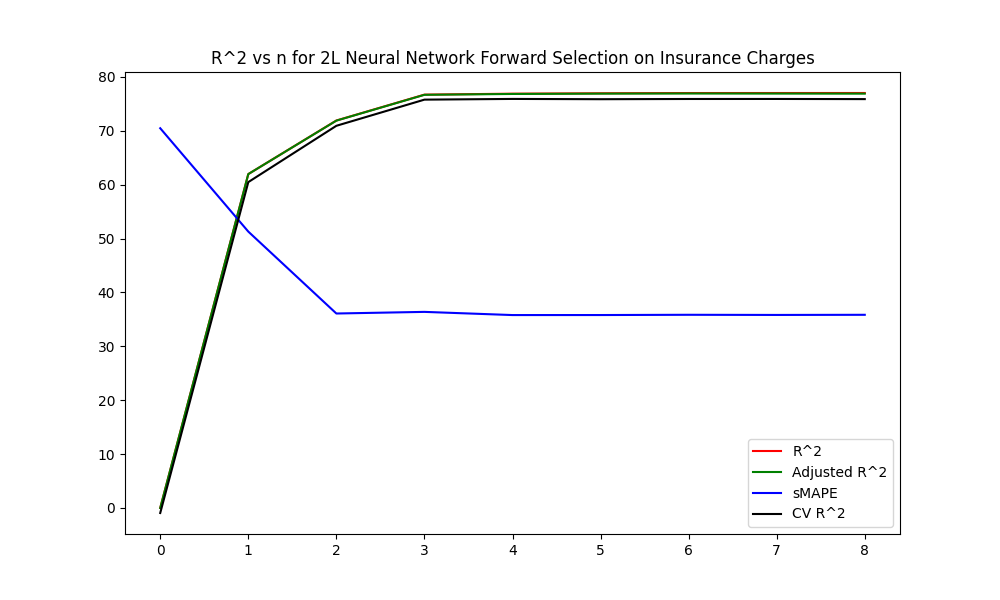
\includegraphics[width=\textwidth]{../Insurance_Charges_Plots/NN_2L_rSq_Forward.png}
     \end{subfigure}
     \hfill
     \begin{subfigure}[b]{0.49\textwidth}
         \centering
         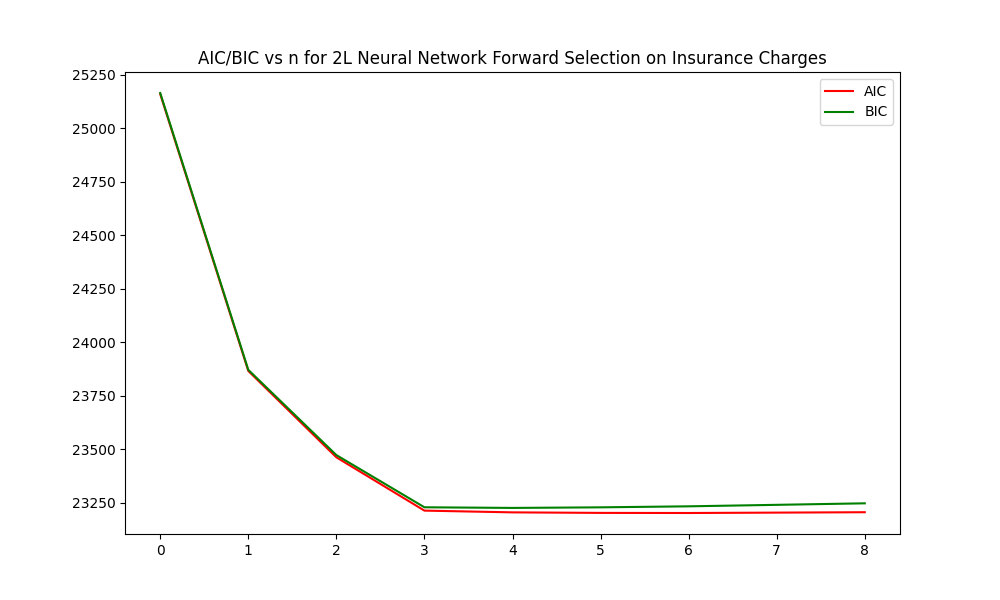
\includegraphics[width=\textwidth]{../Insurance_Charges_Plots/NN_2L_AIC_BIC_Forward.png}
     \end{subfigure}
     
     \caption{Insurance Charges 2 Layer Neural Network Forward Selection Quality of Fit Metrics\\ Left: $R^2$, Right: AIC/BIC}
     \label{fig:Insurance Charges 2 Layer Neural Network Forward Selection Quality of Fit Metrics}
\end{figure}

\noindent Backward Elimination Reversed: Null, smoker yes, age, bmi, children, region southeast, region southwest, sex male, region northwest

\begin{figure}[H]
     \centering
     \captionsetup{justification=centering}
     \begin{subfigure}[b]{0.49\textwidth}
         \centering
         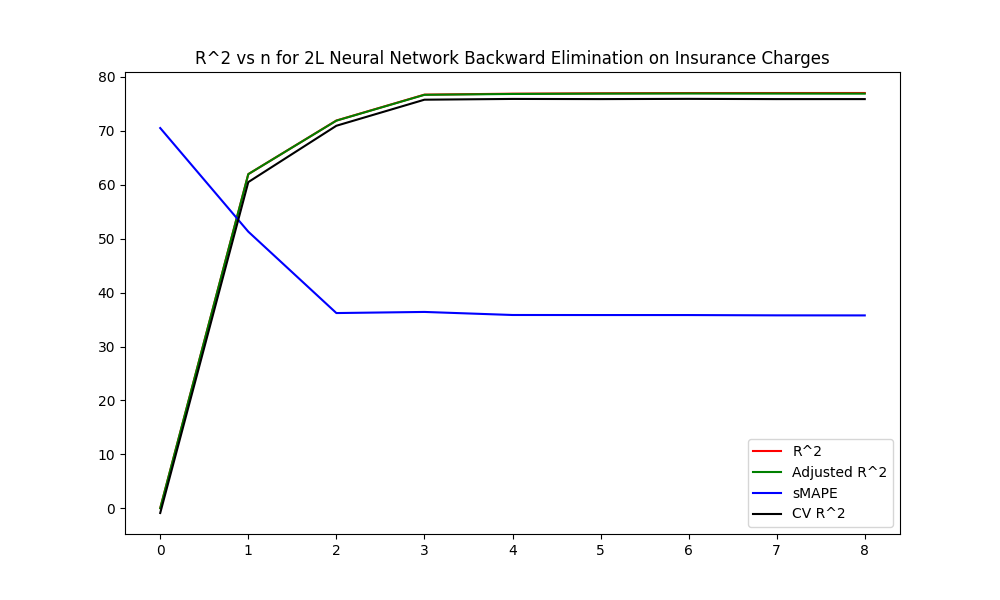
\includegraphics[width=\textwidth]{../Insurance_Charges_Plots/NN_2L_rSq_Backward.png}
     \end{subfigure}
     \hfill
     \begin{subfigure}[b]{0.49\textwidth}
         \centering
         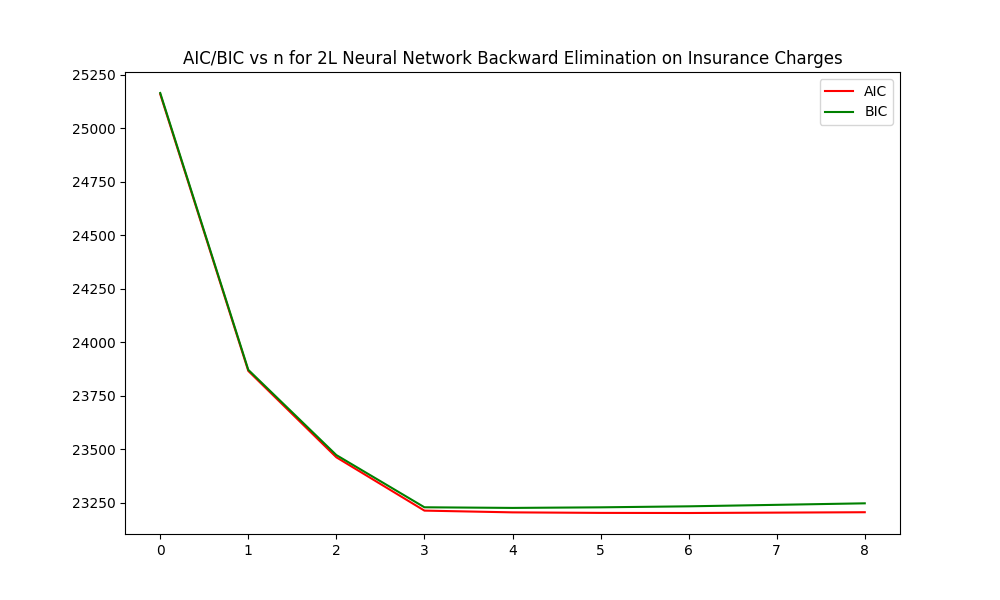
\includegraphics[width=\textwidth]{../Insurance_Charges_Plots/NN_2L_AIC_BIC_Backward.png}
     \end{subfigure}
     
     \caption{Insurance Charges 2 Layer Neural Network Backward Elimination Quality of Fit Metrics\\ Left: $R^2$, Right: AIC/BIC}
     \label{fig:Insurance Charges 2 Layer Neural Network Backward Elimination Quality of Fit Metrics}
\end{figure}

\noindent Stepwise Selection: Null, smoker yes, age, bmi, children, region southeast, region southwest

\begin{figure}[H]
     \centering
     \captionsetup{justification=centering}
     \begin{subfigure}[b]{0.49\textwidth}
         \centering
         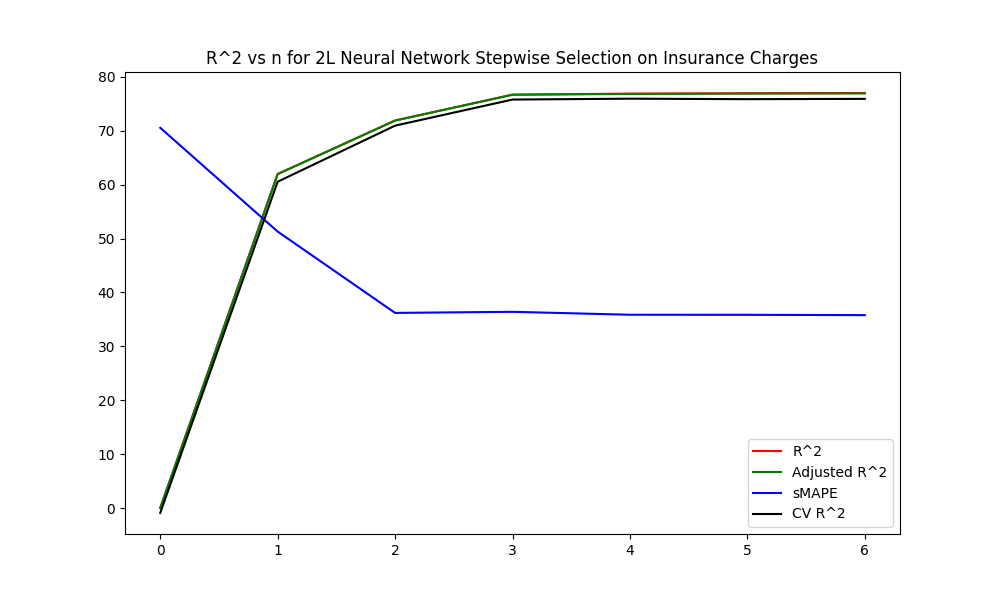
\includegraphics[width=\textwidth]{../Insurance_Charges_Plots/NN_2L_rSq_Stepwise.png}
     \end{subfigure}
     \hfill
     \begin{subfigure}[b]{0.49\textwidth}
         \centering
         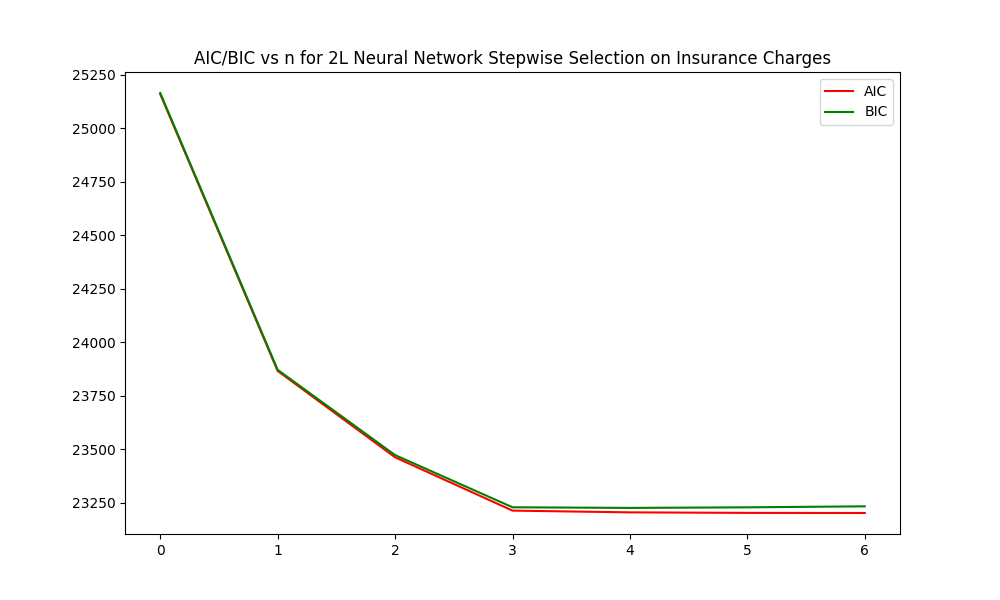
\includegraphics[width=\textwidth]{../Insurance_Charges_Plots/NN_2L_AIC_BIC_Stepwise.png}
     \end{subfigure}
     
     \caption{Insurance Charges 2 Layer Neural Network Stepwise Selection Quality of Fit Metrics\\ Left: $R^2$, Right: AIC/BIC}
     \label{fig:Insurance Charges 2 Layer Neural Network Stepwise Selection Quality of Fit Metrics}
\end{figure}

%%%%%%%%%%%%%%%%%%%%%%%%%%%%%%%%%%%%%%%%%%%%%%%%%%%%%%%%%%%%
%%%%%%%%%%%%%%%%%%%%%%%%%%%%%%%%%%%%%%%%%%%%%%%%%%%%%%%%%%%%
%%%%%%%%%%%%%%%%%%%%%%%%%%%%%%%%%%%%%%%%%%%%%%%%%%%%%%%%%%%%
%%%%%%%%%%%%%%%%%%%%%%%%%%%%%%%%%%%%%%%%%%%%%%%%%%%%%%%%%%%%
%%%%%%%%%%%%%%%%%%%%%%%%%%%%%%%%%%%%%%%%%%%%%%%%%%%%%%%%%%%%
%%%%%%%%%%%%%%%%%%%%%%%%%%%%%%%%%%%%%%%%%%%%%%%%%%%%%%%%%%%%

\subsection{Three Layer Neural Network}

\subsubsection{Quality of Fit}

Insurance Charges NN 3L hidden activation: ELU, output activation: Identity, hidden 1: 8, lr: 5e-02

\begin{figure}[H]
     \centering
     \captionsetup{justification=centering}
     \begin{subfigure}[b]{0.49\textwidth}
         \centering
         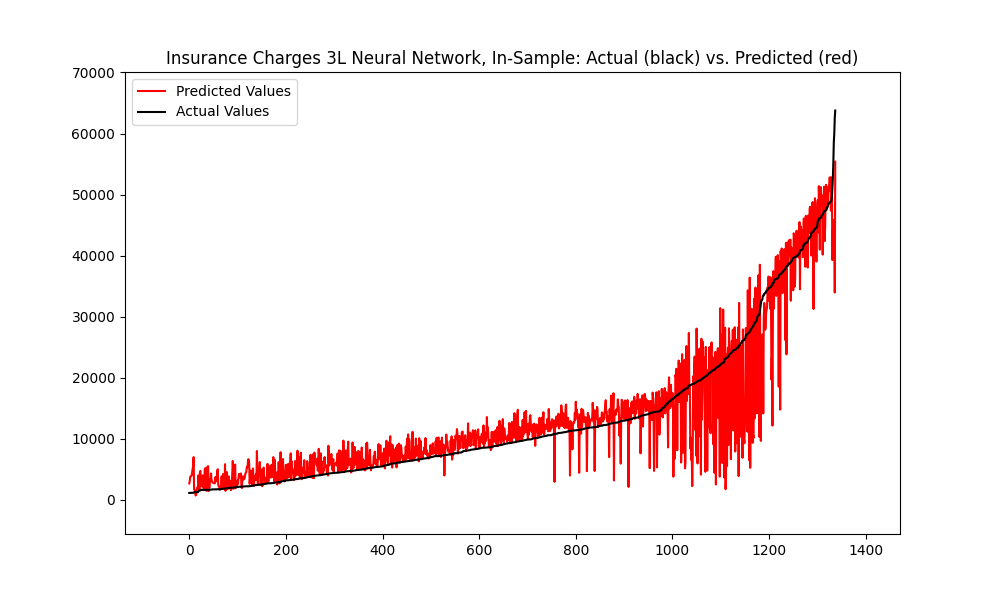
\includegraphics[width=\textwidth]{../Insurance_Charges_Plots/NN_3L_In_Sample.png}
     \end{subfigure}
     \hfill
     \begin{subfigure}[b]{0.49\textwidth}
         \centering
         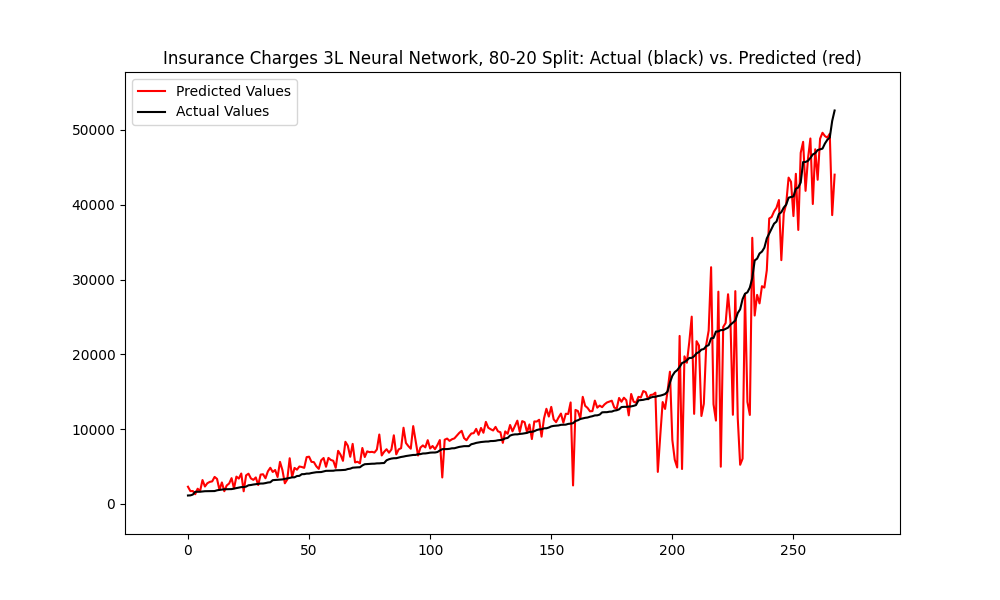
\includegraphics[width=\textwidth]{../Insurance_Charges_Plots/NN_3L_80_20.png}
     \end{subfigure}
     
     \caption{Insurance Charges 3 Layer Neural Network Plots\\ Left: In-Sample, Right: Out-of-Sample\\ black: actual y-values, red: predicted y-values}
     \label{fig:Insurance Charges 3 Layer Neural Network Plots}
\end{figure}

\begin{table}[H]
\centering
\caption{Insurance Charges 3L Neural Network}
\label{tab:Insurance Charges 3L Neural Network}
\begin{tabular}{|c|c|c|}\hline
Metric & In-Sample & 80-20 Split \\ \hline \hline
rSq & 0.8535 & 0.8926 \\ \hline
rSqBar & 0.8527 & 0.8897 \\ \hline
sst & 1.961e+11 & 4.265e+10 \\ \hline
sse & 2.873e+10 & 4.58e+09 \\ \hline
sde & 4648 & 4197 \\ \hline
mse0 & 2.147e+07 & 1.709e+07 \\ \hline
rmse & 4634 & 4134 \\ \hline
mae & 2814 & 2401 \\ \hline
smape & 27.01 & 23.25 \\ \hline
m & 1338 & 268 \\ \hline
dfr & 8 & 8 \\ \hline
df & 1330 & 260 \\ \hline
fStat & 968.4 & 270.2 \\ \hline
aic & 2.26e+04 & 4479 \\ \hline
bic & 2.265e+04 & 4508 \\ \hline
\end{tabular}
\end{table}

\begin{table}[H]
\centering
\caption{Insurance Charges 3L Neural Network CV}
\label{tab:Insurance Charges 3L Neural Network CV}
\begin{tabular}{|c|c|c|c|c|c|}\hline
Metric & num folds & min & max & mean & stdev \\ \hline \hline
rSq & 5 & 0.7925 & 0.8834 & 0.8427 & 0.03985 \\ \hline
rSqBar & 5 & 0.7869 & 0.8803 & 0.8384 & 0.04093 \\ \hline
sst & 5 & 2.986e+10 & 4.265e+10 & 3.902e+10 & 4.668e+09 \\ \hline
sse & 5 & 4.971e+09 & 8.555e+09 & 6.03e+09 & 1.333e+09 \\ \hline
sde & 5 & 4372 & 5747 & 4793 & 508.9 \\ \hline
mse0 & 5 & 1.855e+07 & 3.204e+07 & 2.254e+07 & 5.012e+06 \\ \hline
rmse & 5 & 4307 & 5660 & 4721 & 501.2 \\ \hline
mae & 5 & 2347 & 3363 & 2831 & 337.5 \\ \hline
smape & 5 & 24.27 & 34.1 & 28.2 & 3.861 \\ \hline
m & 5 & 267 & 268 & 267.6 & 0.4899 \\ \hline
dfr & 5 & 8 & 8 & 8 & 0 \\ \hline
df & 5 & 259 & 260 & 259.6 & 0.4899 \\ \hline
fStat & 5 & 124.1 & 246.3 & 186.8 & 51.41 \\ \hline
aic & 5 & 4501 & 4630 & 4541 & 49.82 \\ \hline
bic & 5 & 4530 & 4659 & 4570 & 49.81 \\ \hline
\end{tabular}
\end{table}

\subsubsection{Feature Selection}

\noindent Forward Selection: Null, smoker yes, bmi, age, children, region southwest, region southeast, region northwest, sex male

\begin{figure}[H]
     \centering
     \captionsetup{justification=centering}
     \begin{subfigure}[b]{0.49\textwidth}
         \centering
         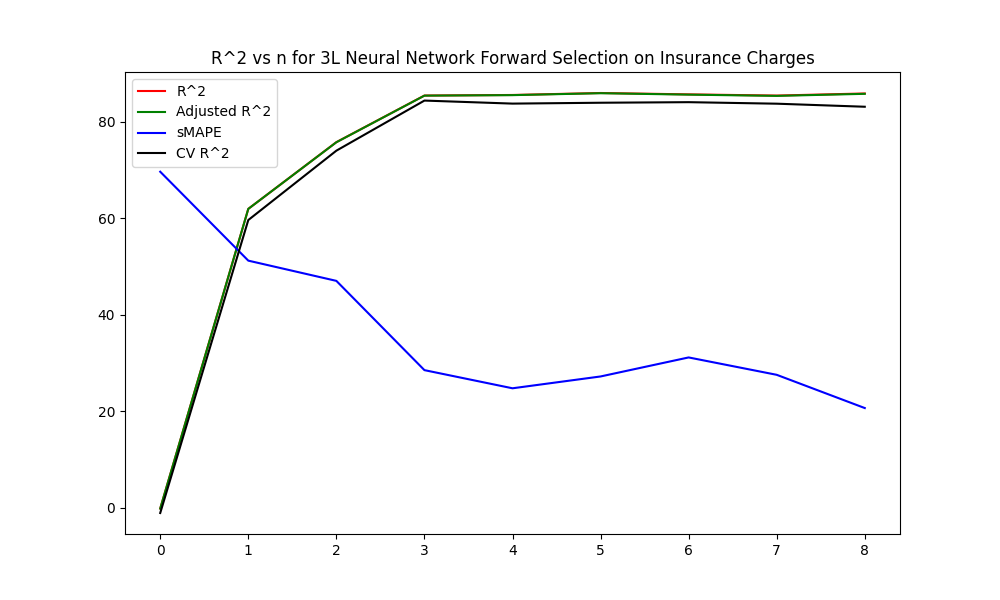
\includegraphics[width=\textwidth]{../Insurance_Charges_Plots/NN_3L_rSq_Forward.png}
     \end{subfigure}
     \hfill
     \begin{subfigure}[b]{0.49\textwidth}
         \centering
         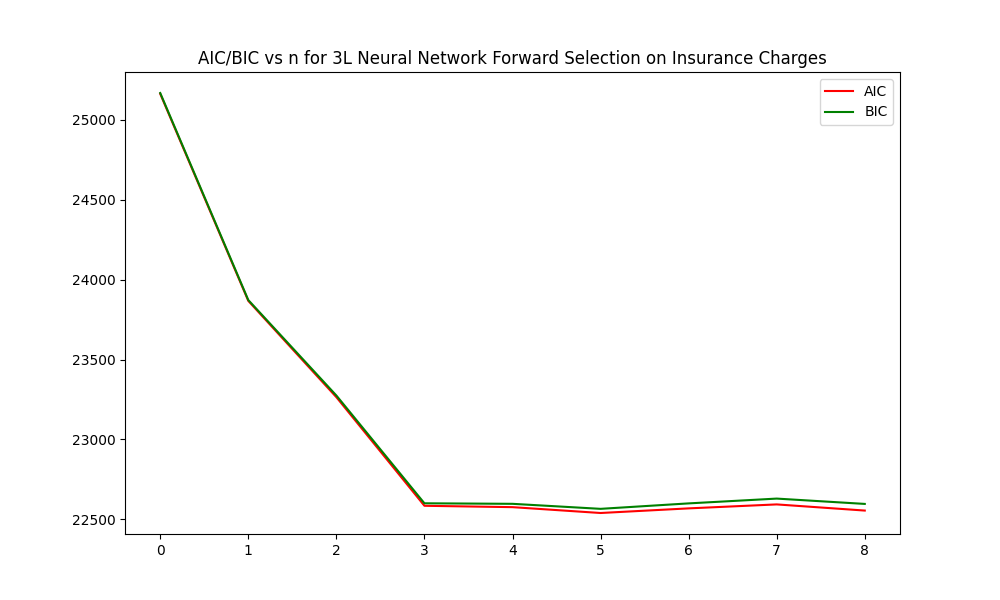
\includegraphics[width=\textwidth]{../Insurance_Charges_Plots/NN_3L_AIC_BIC_Forward.png}
     \end{subfigure}
     
     \caption{Insurance Charges 3 Layer Neural Network Forward Selection Quality of Fit Metrics\\ Left: $R^2$, Right: AIC/BIC}
     \label{fig:Insurance Charges 3 Layer Neural Network Forward Selection Quality of Fit Metrics}
\end{figure}

\noindent Backward Elimination Reversed: Null, smoker yes, bmi, age, region northwest, children, region southwest, sex male, region southeast

\begin{figure}[H]
     \centering
     \captionsetup{justification=centering}
     \begin{subfigure}[b]{0.49\textwidth}
         \centering
         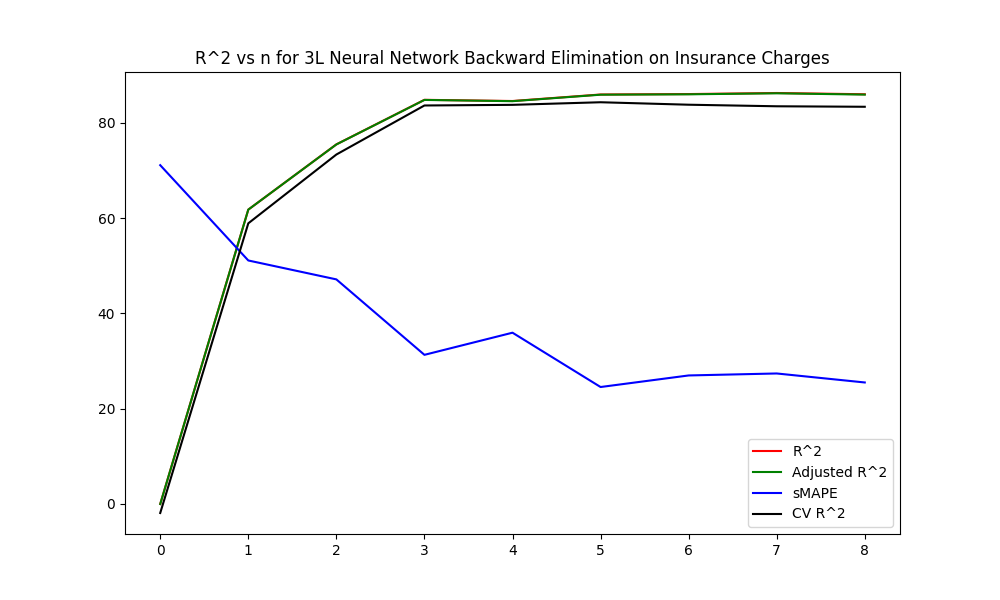
\includegraphics[width=\textwidth]{../Insurance_Charges_Plots/NN_3L_rSq_Backward.png}
     \end{subfigure}
     \hfill
     \begin{subfigure}[b]{0.49\textwidth}
         \centering
         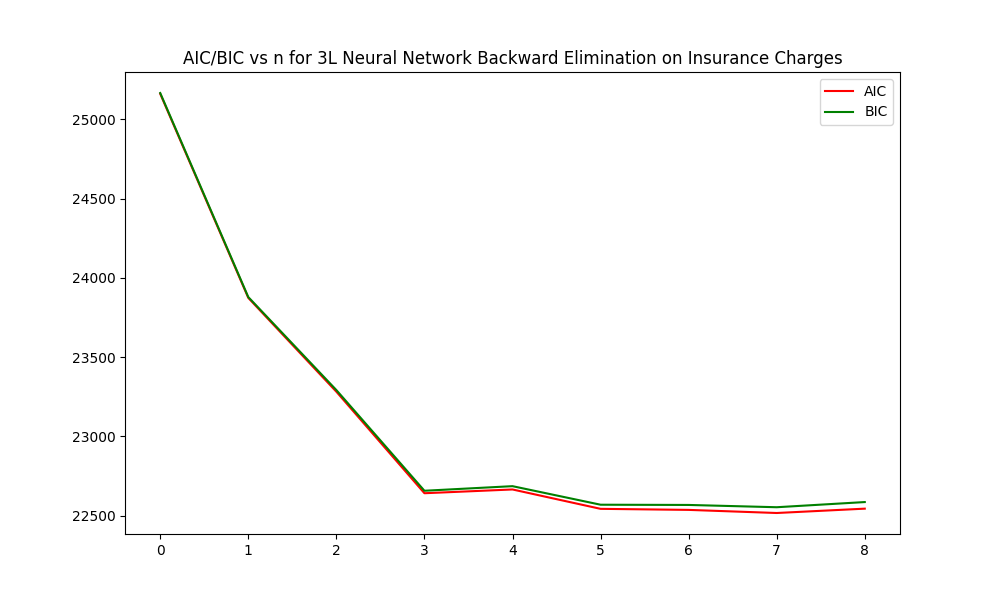
\includegraphics[width=\textwidth]{../Insurance_Charges_Plots/NN_3L_AIC_BIC_Backward.png}
     \end{subfigure}
     
     \caption{Insurance Charges 3 Layer Neural Network Backward Elimination Quality of Fit Metrics\\ Left: $R^2$, Right: AIC/BIC}
     \label{fig:Insurance Charges 3 Layer Neural Network Backward Elimination Quality of Fit Metrics}
\end{figure}

\noindent Stepwise Selection: Null, smoker yes, bmi, age, children

\begin{figure}[H]
     \centering
     \captionsetup{justification=centering}
     \begin{subfigure}[b]{0.49\textwidth}
         \centering
         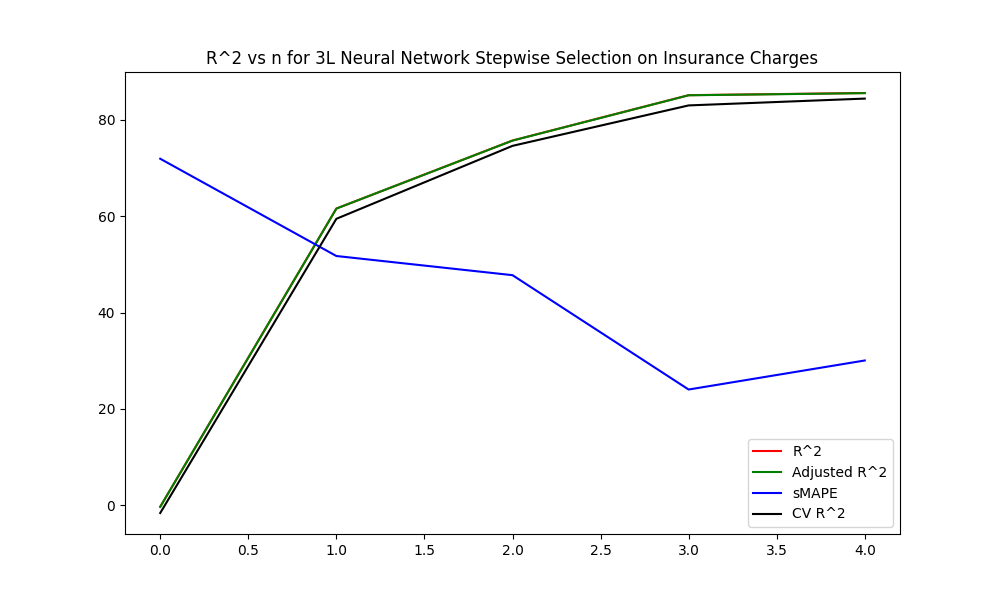
\includegraphics[width=\textwidth]{../Insurance_Charges_Plots/NN_3L_rSq_Stepwise.png}
     \end{subfigure}
     \hfill
     \begin{subfigure}[b]{0.49\textwidth}
         \centering
         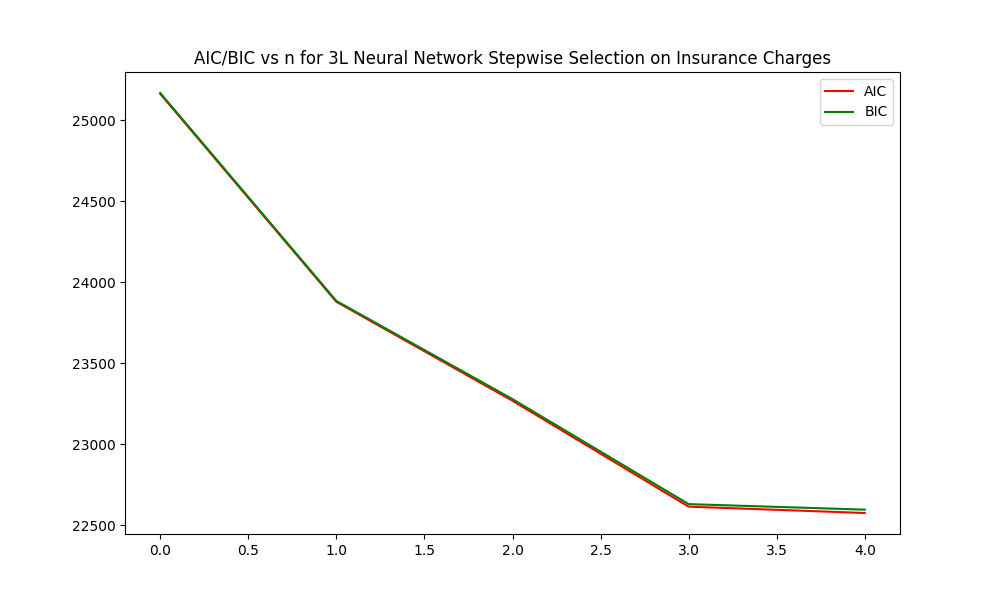
\includegraphics[width=\textwidth]{../Insurance_Charges_Plots/NN_3L_AIC_BIC_Stepwise.png}
     \end{subfigure}
     
     \caption{Insurance Charges 3 Layer Neural Network Stepwise Selection Quality of Fit Metrics\\ Left: $R^2$, Right: AIC/BIC}
     \label{fig:Insurance Charges 3 Layer Neural Network Stepwise Selection Quality of Fit Metrics}
\end{figure}

%%%%%%%%%%%%%%%%%%%%%%%%%%%%%%%%%%%%%%%%%%%%%%%%%%%%%%%%%%%%
%%%%%%%%%%%%%%%%%%%%%%%%%%%%%%%%%%%%%%%%%%%%%%%%%%%%%%%%%%%%
%%%%%%%%%%%%%%%%%%%%%%%%%%%%%%%%%%%%%%%%%%%%%%%%%%%%%%%%%%%%
%%%%%%%%%%%%%%%%%%%%%%%%%%%%%%%%%%%%%%%%%%%%%%%%%%%%%%%%%%%%
%%%%%%%%%%%%%%%%%%%%%%%%%%%%%%%%%%%%%%%%%%%%%%%%%%%%%%%%%%%%
%%%%%%%%%%%%%%%%%%%%%%%%%%%%%%%%%%%%%%%%%%%%%%%%%%%%%%%%%%%%

\subsection{Four Layer Neural Network}

\subsubsection{Quality of Fit}

Insurance Charges NN 4L hidden activation 1: ELU, hidden activation 2: ELU, output activation: Identity, hidden 1: 256, hidden 2: 32, lr: 5e-03

\begin{figure}[H]
     \centering
     \captionsetup{justification=centering}
     \begin{subfigure}[b]{0.49\textwidth}
         \centering
         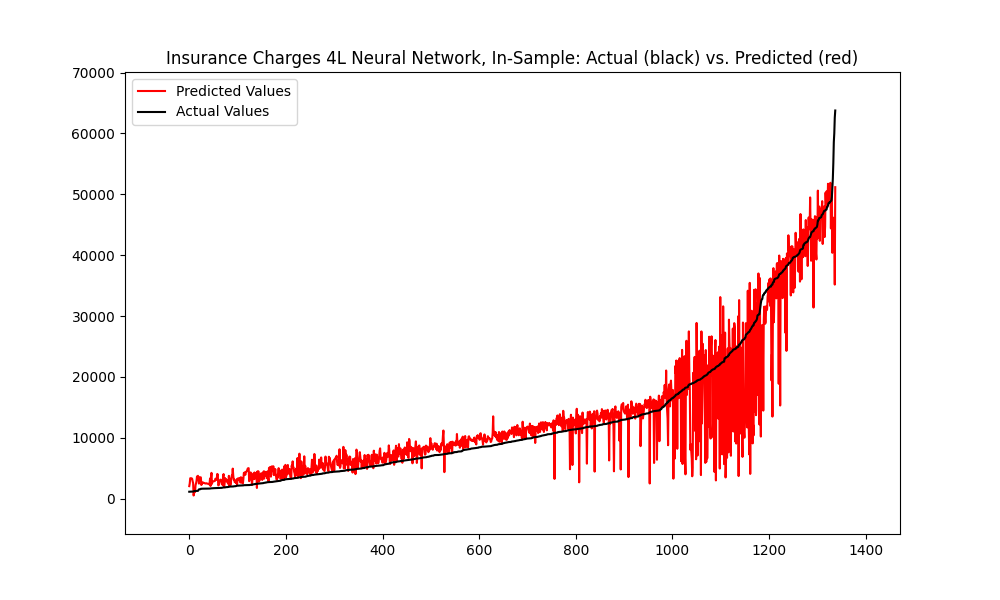
\includegraphics[width=\textwidth]{../Insurance_Charges_Plots/NN_4L_In_Sample.png}
     \end{subfigure}
     \hfill
     \begin{subfigure}[b]{0.49\textwidth}
         \centering
         
\includegraphics[width=\textwidth]{../Insurance_Charges_Plots/NN_4L_80_20.png}
     \end{subfigure}
     
     \caption{Insurance Charges 4 Layer Neural Network Plots\\ Left: In-Sample, Right: Out-of-Sample\\ black: actual y-values, red: predicted y-values}
     \label{fig:Insurance Charges 4 Layer Neural Network Plots}
\end{figure}

\begin{table}[H]
\centering
\caption{Insurance Charges 4L Neural Network}
\label{tab:Insurance Charges 4L Neural Network}
\begin{tabular}{|c|c|c|}\hline
Metric & In-Sample & 80-20 Split \\ \hline \hline
rSq & 0.8674 & 0.884 \\ \hline
rSqBar & 0.8667 & 0.8809 \\ \hline
sst & 1.961e+11 & 4.265e+10 \\ \hline
sse & 2.6e+10 & 4.947e+09 \\ \hline
sde & 4421 & 4362 \\ \hline
mse0 & 1.943e+07 & 1.846e+07 \\ \hline
rmse & 4408 & 4296 \\ \hline
mae & 2557 & 2900 \\ \hline
smape & 25.04 & 28.72 \\ \hline
m & 1338 & 268 \\ \hline
dfr & 8 & 8 \\ \hline
df & 1330 & 260 \\ \hline
fStat & 1088 & 247.7 \\ \hline
aic & 2.247e+04 & 4500 \\ \hline
bic & 2.251e+04 & 4529 \\ \hline
\end{tabular}
\end{table}

\begin{table}[H]
\centering
\caption{Insurance Charges 4L Neural Network CV}
\label{tab:Insurance Charges 4L Neural Network CV}
\begin{tabular}{|c|c|c|c|c|c|}\hline
Metric & num folds & min & max & mean & stdev \\ \hline \hline
rSq & 5 & 0.7924 & 0.8866 & 0.842 & 0.0407 \\ \hline
rSqBar & 5 & 0.7868 & 0.8836 & 0.8377 & 0.0418 \\ \hline
sst & 5 & 2.986e+10 & 4.265e+10 & 3.902e+10 & 4.668e+09 \\ \hline
sse & 5 & 4.835e+09 & 8.653e+09 & 6.057e+09 & 1.381e+09 \\ \hline
sde & 5 & 4312 & 5780 & 4802 & 527.6 \\ \hline
mse0 & 5 & 1.804e+07 & 3.241e+07 & 2.264e+07 & 5.194e+06 \\ \hline
rmse & 5 & 4248 & 5693 & 4730 & 519.6 \\ \hline
mae & 5 & 2476 & 3114 & 2786 & 228.3 \\ \hline
smape & 5 & 25.74 & 29.89 & 27.06 & 1.484 \\ \hline
m & 5 & 267 & 268 & 267.6 & 0.4899 \\ \hline
dfr & 5 & 8 & 8 & 8 & 0 \\ \hline
df & 5 & 259 & 260 & 259.6 & 0.4899 \\ \hline
fStat & 5 & 124 & 254.1 & 186.6 & 53.39 \\ \hline
aic & 5 & 4494 & 4633 & 4542 & 51.25 \\ \hline
bic & 5 & 4523 & 4662 & 4570 & 51.24 \\ \hline
\end{tabular}
\end{table}

\subsubsection{Feature Selection}

\noindent Forward Selection: Null, smoker yes, bmi, age, children, region northwest, sex male, region southwest, region southeast

\begin{figure}[H]
     \centering
     \captionsetup{justification=centering}
     \begin{subfigure}[b]{0.49\textwidth}
         \centering
         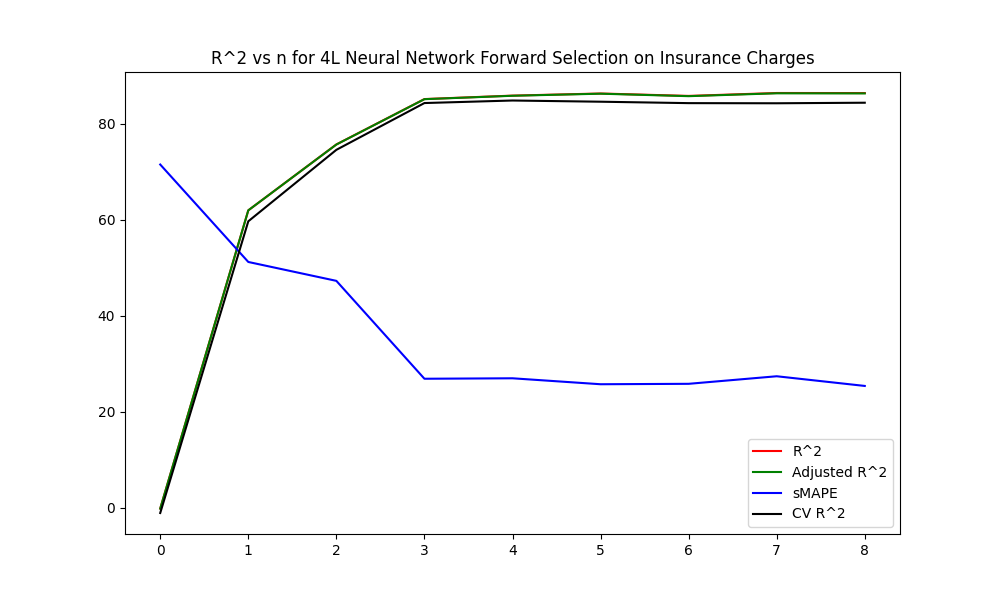
\includegraphics[width=\textwidth]{../Insurance_Charges_Plots/NN_4L_rSq_Forward.png}
     \end{subfigure}
     \hfill
     \begin{subfigure}[b]{0.49\textwidth}
         \centering
         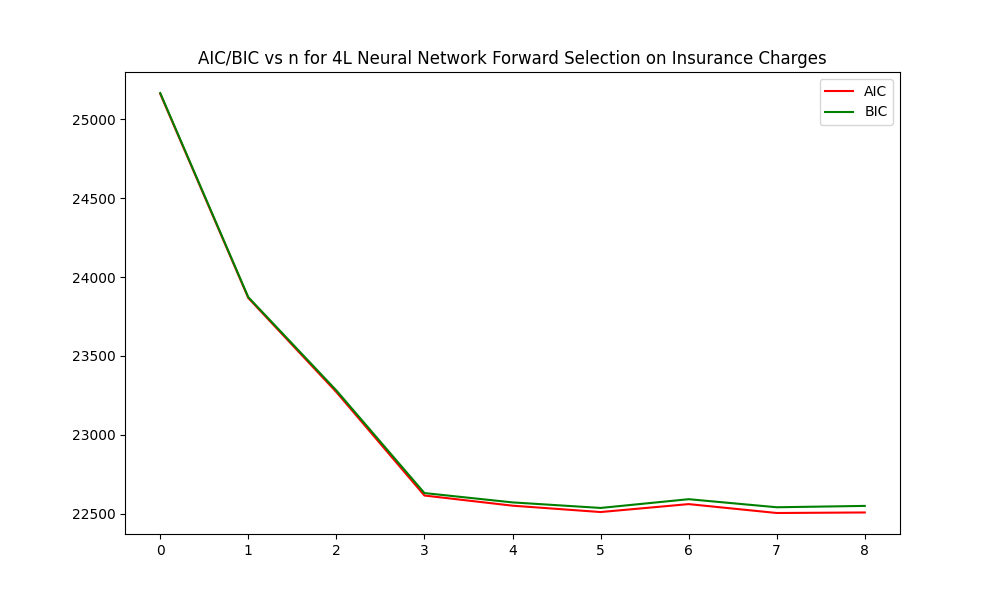
\includegraphics[width=\textwidth]{../Insurance_Charges_Plots/NN_4L_AIC_BIC_Forward.png}
     \end{subfigure}
     
     \caption{Insurance Charges 4 Layer Neural Network Forward Selection Quality of Fit Metrics\\ Left: $R^2$, Right: AIC/BIC}
     \label{fig:Insurance Charges 4 Layer Neural Network Forward Selection Quality of Fit Metrics}
\end{figure}

\noindent Backward Elimination Reversed: Null, smoker yes, bmi, age, children, region southeast, region southwest, sex male, region northwest

\begin{figure}[H]
     \centering
     \captionsetup{justification=centering}
     \begin{subfigure}[b]{0.49\textwidth}
         \centering
         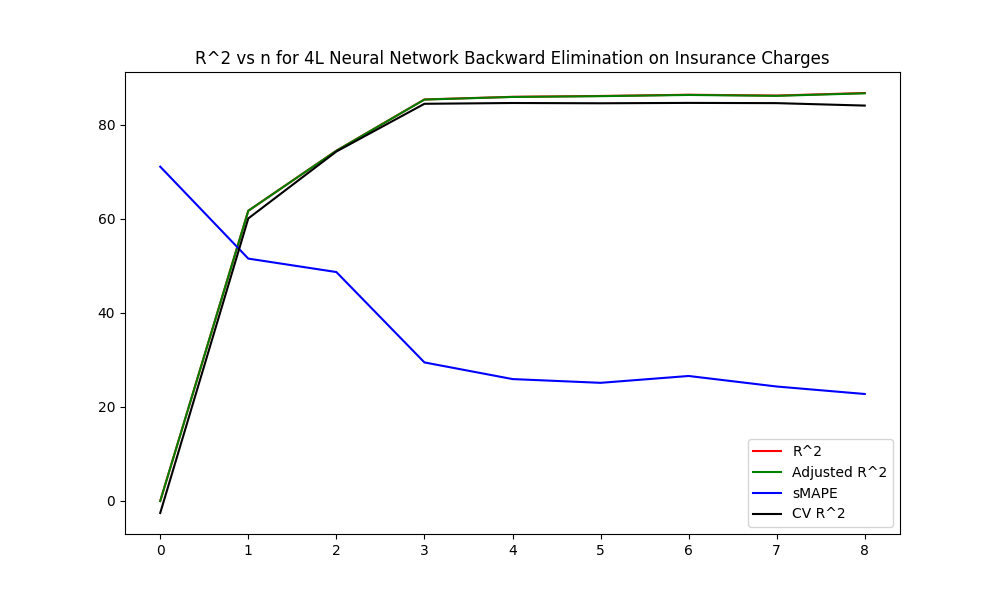
\includegraphics[width=\textwidth]{../Insurance_Charges_Plots/NN_4L_rSq_Backward.png}
     \end{subfigure}
     \hfill
     \begin{subfigure}[b]{0.49\textwidth}
         \centering
         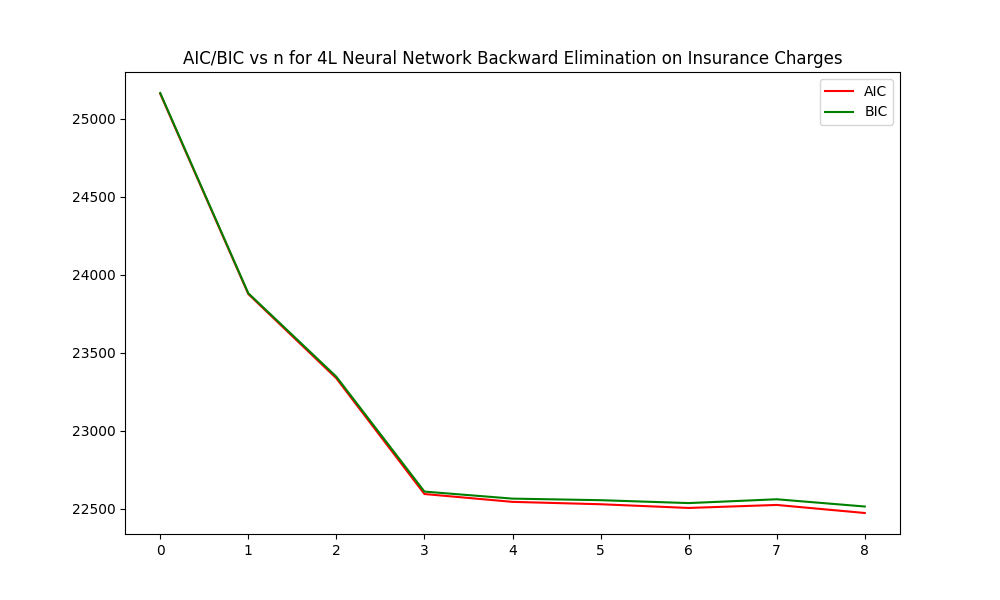
\includegraphics[width=\textwidth]{../Insurance_Charges_Plots/NN_4L_AIC_BIC_Backward.png}
     \end{subfigure}
     
     \caption{Insurance Charges 4 Layer Neural Network Backward Elimination Quality of Fit Metrics\\ Left: $R^2$, Right: AIC/BIC}
     \label{fig:Insurance Charges 4 Layer Neural Network Backward Elimination Quality of Fit Metrics}
\end{figure}

\noindent Stepwise Selection: Null, smoker yes, bmi, age, children, region southeast, region southwest, sex male

\begin{figure}[H]
     \centering
     \captionsetup{justification=centering}
     \begin{subfigure}[b]{0.49\textwidth}
         \centering
         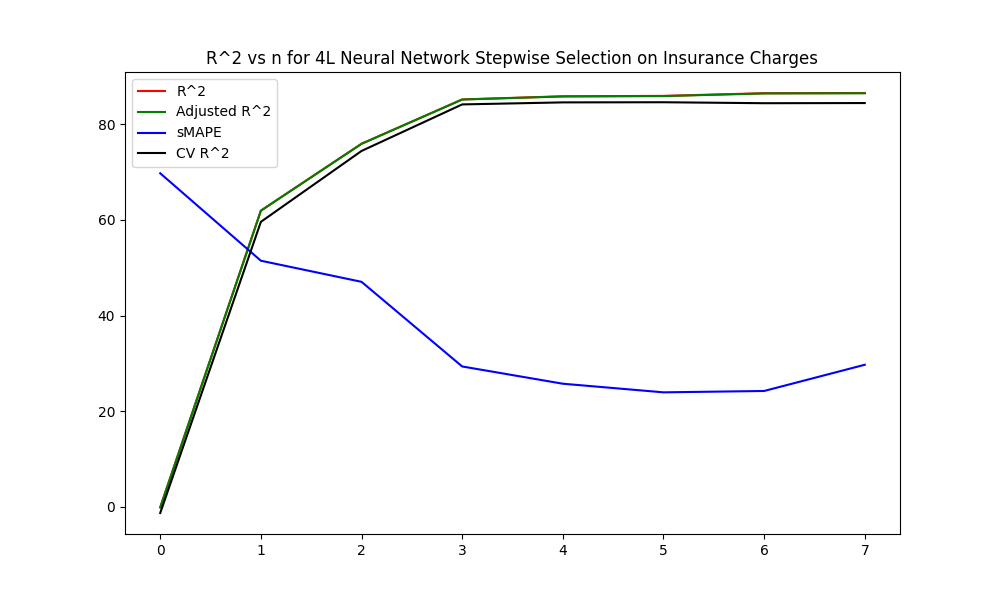
\includegraphics[width=\textwidth]{../Insurance_Charges_Plots/NN_4L_rSq_Stepwise.png}
     \end{subfigure}
     \hfill
     \begin{subfigure}[b]{0.49\textwidth}
         \centering
         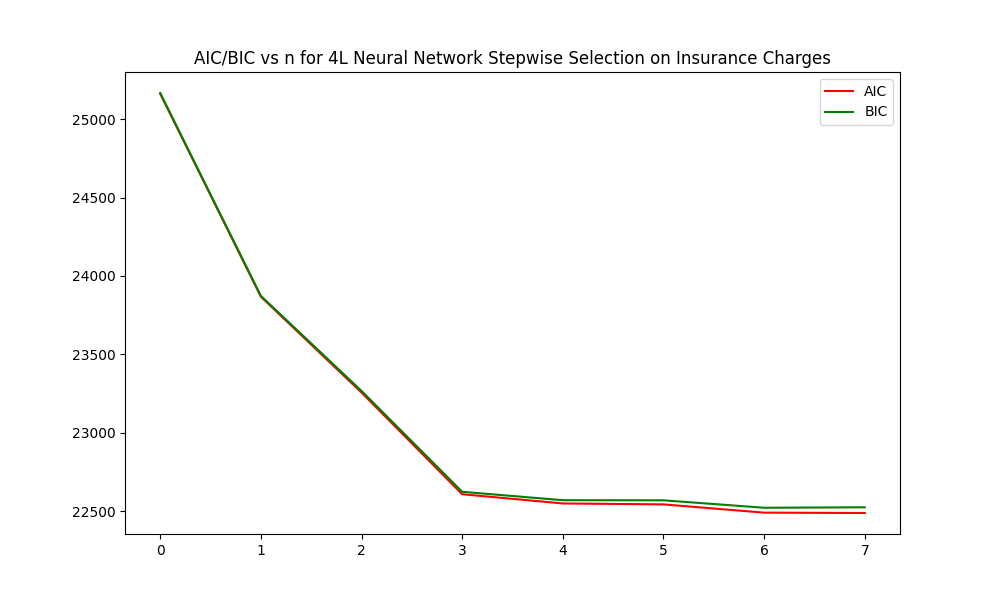
\includegraphics[width=\textwidth]{../Insurance_Charges_Plots/NN_4L_AIC_BIC_Stepwise.png}
     \end{subfigure}
     
     \caption{Insurance Charges 4 Layer Neural Network Stepwise Selection Quality of Fit Metrics\\ Left: $R^2$, Right: AIC/BIC}
     \label{fig:Insurance Charges 4 Layer Neural Network Stepwise Selection Quality of Fit Metrics}
\end{figure}

\subsection{Model Comparison}

\begin{table}[H]
\centering
\caption{Insurance Charges In-Sample QoF Comparison}
\label{tab:Insurance Charges In-Sample QoF Comparison}
\resizebox{\textwidth}{!}{
\begin{tabular}{|c|c|c|c|c|c|c|c|c|c|c|}\hline
Metric & Reg & Ridge & Lasso & Sqrt & Log1p & Box-Cox & Order 2 & NN 2L & NN 3L & NN 4L \\ \hline \hline
rSq & 0.7509 & 0.7509 & 0.7509 & 0.7527 & 0.5228 & 0.7527 & 0.8477 & 0.7703 & 0.8535 & 0.8674 \\ \hline
rSqBar & 0.7494 & 0.7495 & 0.7496 & 0.7512 & 0.5199 & 0.7512 & 0.8406 & 0.7691 & 0.8527 & 0.8667 \\ \hline
sst & 1.961e+11 & 1.961e+11 & 1.961e+11 & 1.961e+11 & 1.961e+11 & 1.961e+11 & 1.961e+11 & 1.961e+11 & 1.961e+11 & 1.961e+11 \\ \hline
sse & 4.884e+10 & 4.885e+10 & 4.884e+10 & 4.85e+10 & 9.357e+10 & 4.85e+10 & 2.986e+10 & 4.504e+10 & 2.873e+10 & 2.6e+10 \\ \hline
sde & 6062 & 6061 & 6060 & 6041 & 8391 & 6041 & 4835 & 5819 & 4648 & 4421 \\ \hline
mse0 & 3.65e+07 & 3.651e+07 & 3.65e+07 & 3.625e+07 & 6.993e+07 & 3.625e+07 & 2.232e+07 & 3.366e+07 & 2.147e+07 & 1.943e+07 \\ \hline
rmse & 6042 & 6042 & 6042 & 6020 & 8363 & 6020 & 4724 & 5802 & 4634 & 4408 \\ \hline
mae & 4171 & 4182 & 4170 & 3614 & 4220 & 3614 & 2833 & 3996 & 2814 & 2557 \\ \hline
smape & 37.81 & 37.68 & 37.72 & 27.69 & 26.29 & 27.69 & 26.43 & 35.78 & 27.01 & 25.04 \\ \hline
m & 1338 & 1338 & 1338 & 1338 & 1338 & 1338 & 1338 & 1338 & 1338 & 1338 \\ \hline
dfr & 9 & 8 & 8 & 9 & 9 & 9 & 61 & 8 & 8 & 8 \\ \hline
df & 1329 & 1330 & 1330 & 1329 & 1329 & 1329 & 1277 & 1330 & 1330 & 1330 \\ \hline
fStat & 445.2 & 501 & 501.2 & 449.3 & 161.8 & 449.3 & 116.5 & 557.5 & 968.4 & 1088 \\ \hline
aic & 2.332e+04 & 2.331e+04 & 2.331e+04 & 2.331e+04 & 2.419e+04 & 2.331e+04 & 2.276e+04 & 2.321e+04 & 2.26e+04 & 2.247e+04 \\ \hline
bic & 2.336e+04 & 2.336e+04 & 2.336e+04 & 2.335e+04 & 2.423e+04 & 2.335e+04 & 2.308e+04 & 2.325e+04 & 2.265e+04 & 2.251e+04 \\ \hline
\end{tabular}
}
\end{table}

\begin{table}[H]
\centering
\caption{Insurance Charges Out-of-Sample QoF Comparison}
\label{tab:Insurance Charges Out-of-Sample QoF Comparison}
\resizebox{\textwidth}{!}{
\begin{tabular}{|c|c|c|c|c|c|c|c|c|c|c|}\hline
Metric & Reg & Ridge & Lasso & Sqrt & Log1p & Box-Cox & Order 2 & NN 2L & NN 3L & NN 4L \\ \hline \hline
rSq & 0.8 & 0.7993 & 0.7997 & 0.8077 & 0.5468 & 0.8077 & 0.88 & 0.8211 & 0.8926 & 0.884 \\ \hline
rSqBar & 0.7938 & 0.7939 & 0.7943 & 0.8017 & 0.5328 & 0.8017 & 0.8452 & 0.8163 & 0.8897 & 0.8809 \\ \hline
sst & 4.265e+10 & 4.265e+10 & 4.265e+10 & 4.265e+10 & 4.265e+10 & 4.265e+10 & 4.265e+10 & 4.265e+10 & 4.265e+10 & 4.265e+10 \\ \hline
sse & 8.53e+09 & 8.561e+09 & 8.541e+09 & 8.202e+09 & 1.933e+10 & 8.202e+09 & 5.117e+09 & 7.631e+09 & 4.58e+09 & 4.947e+09 \\ \hline
sde & 5739 & 5738 & 5732 & 5627 & 8638 & 5627 & 4972 & 5418 & 4197 & 4362 \\ \hline
mse0 & 3.183e+07 & 3.194e+07 & 3.187e+07 & 3.06e+07 & 7.211e+07 & 3.06e+07 & 1.909e+07 & 2.847e+07 & 1.709e+07 & 1.846e+07 \\ \hline
rmse & 5642 & 5652 & 5645 & 5532 & 8492 & 5532 & 4370 & 5336 & 4134 & 4296 \\ \hline
mae & 3933 & 3951 & 3936 & 3316 & 4213 & 3316 & 2957 & 3668 & 2401 & 2900 \\ \hline
smape & 35.02 & 34.84 & 35.01 & 26.47 & 25.08 & 26.47 & 28.54 & 33.65 & 23.25 & 28.72 \\ \hline
m & 268 & 268 & 268 & 268 & 268 & 268 & 268 & 268 & 268 & 268 \\ \hline
dfr & 9 & 8 & 8 & 9 & 9 & 9 & 61 & 8 & 8 & 8 \\ \hline
df & 259 & 260 & 260 & 259 & 259 & 259 & 207 & 260 & 260 & 260 \\ \hline
fStat & 115.1 & 129.4 & 129.8 & 120.9 & 34.73 & 120.9 & 24.89 & 149.1 & 270.2 & 247.7 \\ \hline
aic & 4648 & 4647 & 4646 & 4637 & 4867 & 4637 & 4615 & 4616 & 4479 & 4500 \\ \hline
bic & 4680 & 4676 & 4675 & 4670 & 4899 & 4670 & 4834 & 4645 & 4508 & 4529 \\ \hline
\end{tabular}
}
\end{table}

\begin{table}[H]
\centering
\caption{Insurance Charges Cross-Validation QoF Comparison}
\label{tab:Insurance Charges Cross-Validation QoF Comparison}
\resizebox{\textwidth}{!}{
\begin{tabular}{|c|c|c|c|c|c|c|c|c|c|c|}\hline
Metric & Reg & Ridge & Lasso & Sqrt & Log1p & Box-Cox & Order 2 & NN 2L & NN 3L & NN 4L \\ \hline \hline
rSq & 0.7401 & 0.7402 & 0.7401 & 0.7447 & 0.5104 & 0.7447 & 0.836 & 0.7589 & 0.8427 & 0.842 \\ \hline
rSqBar & 0.7321 & 0.7332 & 0.7331 & 0.7368 & 0.4953 & 0.7368 & 0.7884 & 0.7524 & 0.8384 & 0.8377 \\ \hline
sst & 3.902e+10 & 3.902e+10 & 3.902e+10 & 3.902e+10 & 3.902e+10 & 3.902e+10 & 3.902e+10 & 3.902e+10 & 3.902e+10 & 3.902e+10 \\ \hline
sse & 9.937e+09 & 9.938e+09 & 9.938e+09 & 9.869e+09 & 1.915e+10 & 9.869e+09 & 6.302e+09 & 9.209e+09 & 6.03e+09 & 6.057e+09 \\ \hline
sde & 6188 & 6177 & 6176 & 6160 & 8578 & 6160 & 5492 & 5942 & 4793 & 4802 \\ \hline
mse0 & 3.714e+07 & 3.714e+07 & 3.714e+07 & 3.689e+07 & 7.159e+07 & 3.689e+07 & 2.356e+07 & 3.442e+07 & 2.254e+07 & 2.264e+07 \\ \hline
rmse & 6083 & 6084 & 6083 & 6055 & 8433 & 6055 & 4826 & 5852 & 4721 & 4730 \\ \hline
mae & 4206 & 4217 & 4206 & 3646 & 4275 & 3646 & 2913 & 4045 & 2831 & 2786 \\ \hline
smape & 38.03 & 37.88 & 37.94 & 27.88 & 26.53 & 27.88 & 26.99 & 36.06 & 28.2 & 27.06 \\ \hline
m & 267.6 & 267.6 & 267.6 & 267.6 & 267.6 & 267.6 & 267.6 & 267.6 & 267.6 & 267.6 \\ \hline
dfr & 9 & 8 & 8 & 9 & 9 & 9 & 61 & 8 & 8 & 8 \\ \hline
df & 258.6 & 259.6 & 259.6 & 258.6 & 258.6 & 258.6 & 206.6 & 259.6 & 259.6 & 259.6 \\ \hline
fStat & 86.05 & 97.06 & 97.17 & 86.85 & 30.29 & 86.85 & 18.49 & 108.3 & 186.8 & 186.6 \\ \hline
aic & 4680 & 4678 & 4678 & 4677 & 4854 & 4677 & 4658 & 4657 & 4541 & 4542 \\ \hline
bic & 4713 & 4707 & 4707 & 4710 & 4887 & 4710 & 4877 & 4686 & 4570 & 4570 \\ \hline
\end{tabular}
}
\end{table}

\end{document}